\chapter{Condensed Matter XUV Transient Absorption Experiments}

\section{Statement of Contribution}
This experiment uses home-made equipment consisting of a XUV-IR Mach-Zhender interferometer, a bright XUV light source, a target chamber and an XUV photon spectrometer. The entire apparatus was designed, built and tested by Gregory Smith and Stephen Hageman. The LabView software controlling the spectrometer's detector was programmed by Kent Talbert. The vacuum system's safety system was designed and programmed by Andrew Piper. The germanium samples were grown by Dr. Yaguo Tang. Transient absorption experiments were done by Gregory Smith and Stephen Hageman. Analysis presented in this document was done by Gregory Smith. Further details on the apparatus and the relevant physics will be discussed in the main dissertation.

\section{Introduction}

\begin{figure}
	\centering
	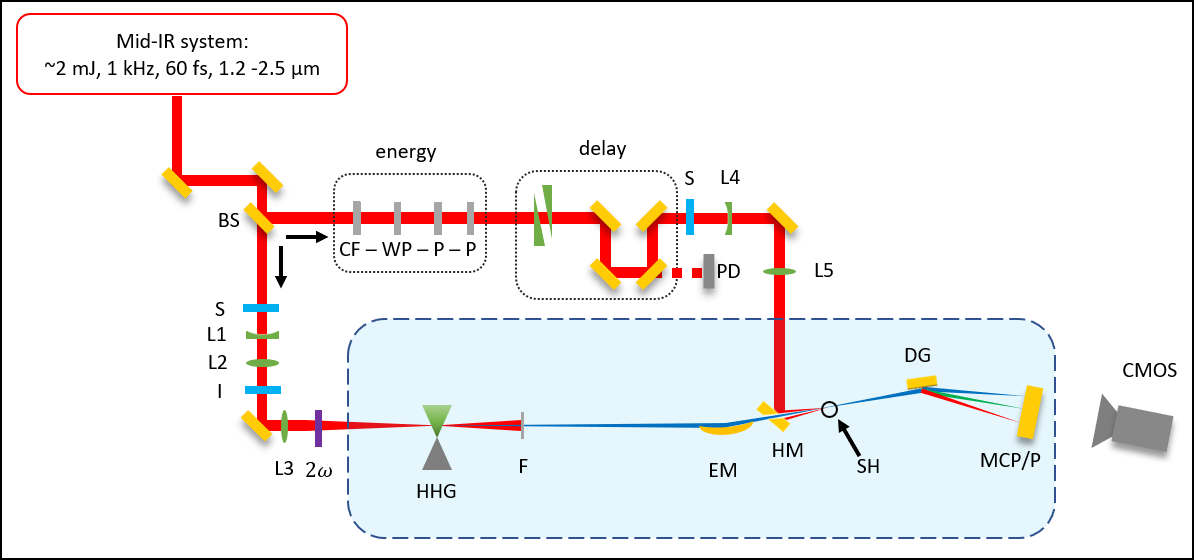
\includegraphics[width=0.95\textwidth]{figures/chap3/beamline_schematic.png}
	\caption{Schematic of the Transient Absorption BeamLine (TABLe). Blue shaded region represents vacuum. BS: beam splitter, S: computer-controlled shutter, L: lens, I: iris, $2\omega$: optics for $2\omega$ generation, HHG: high harmonic generation, F: metallic filter, EM: ellipsoidal mirror, HM: hole mirror, SH: sample holder, CF: long-pass color filter, WP: $\lambda/2$ waveplate, P: wire-grid polarizer, W: delay wedges, PD: photodiode and associated optics, DG: dispersive grating, MCP/P: micro-channel plate and phosphor.}
	\label{fig:beamline_schematic}
\end{figure}

\begin{figure}
	\centering
	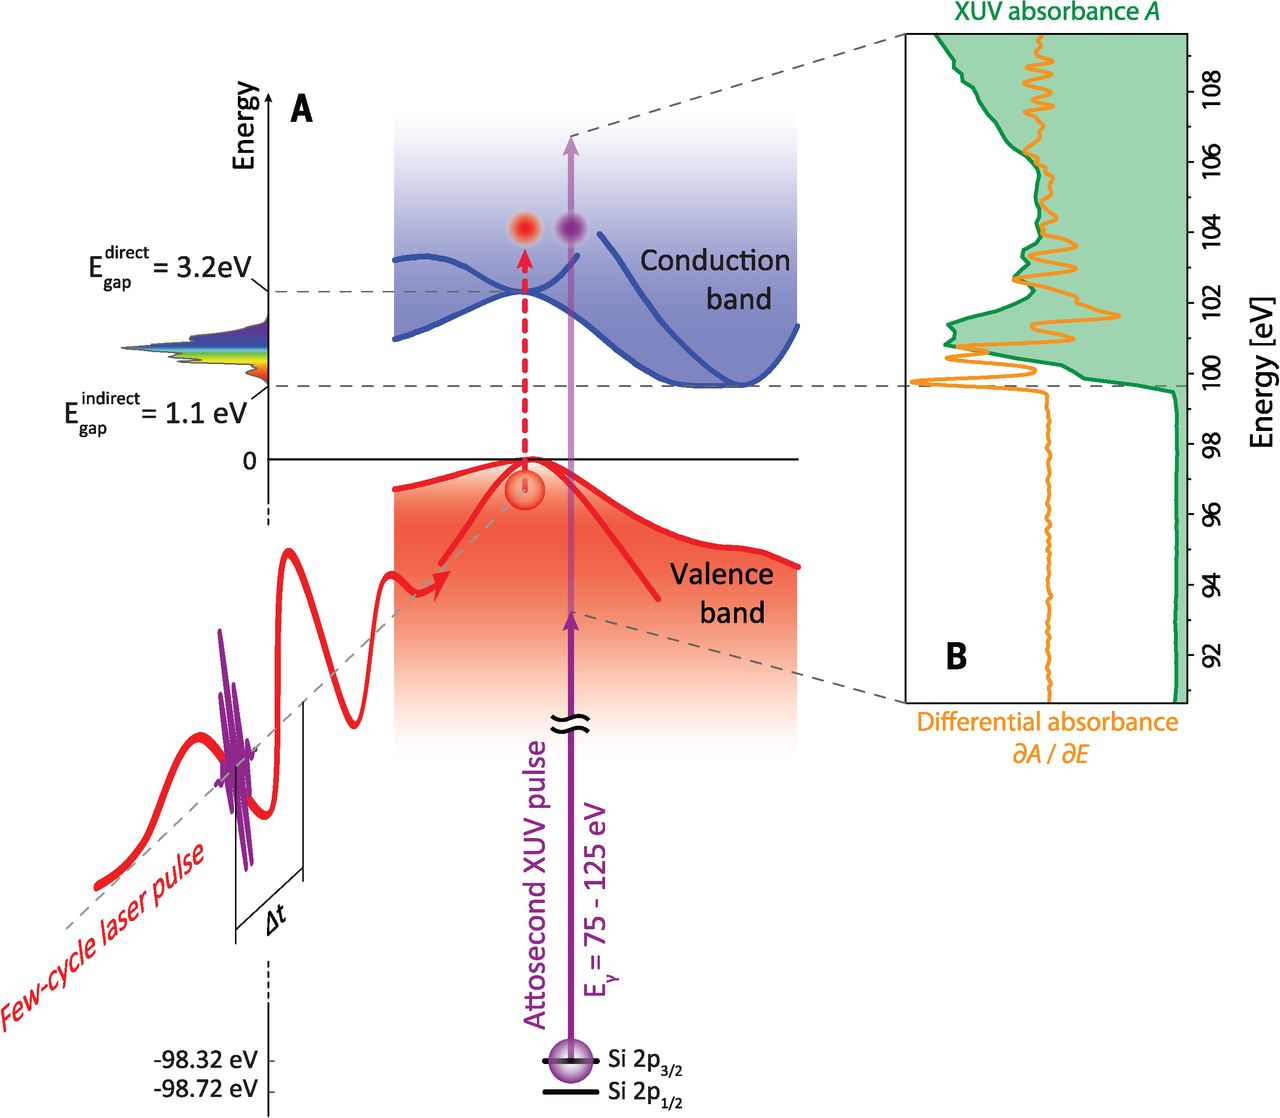
\includegraphics[width=0.75\textwidth]{figures/chap3/ATAS_Cartoon_Si_Leone.jpg}
	\caption{Schematic of an attosecond transient absorption spectroscopy (ATAS) experiment. An IR laser pulse excites electrons in the material, driving them across the band-gap. An XUV pulse passes through the sample after a delay $\Delta t$. The measured XUV absorbance is sensitive to electronic populations and states. Figure taken from \cite{schultzeAttosecondBandgapDynamics2014}.}
	\label{fig:ATAS_Cartoon_Si_Leone}
\end{figure}

We generate extreme ultraviolet (XUV) light using an extremely non-linear process called \textit{high harmonic generation} (HHG). Briefly, the XUV light source can be thought of as a frequency comb spanning from $\sim20$ eV to $\sim50$ eV. The separation between the teeth of the frequency comb is $\omega$, the frequency of our laser light. In the time domain, the XUV is a train of attosecond bursts of broadband light with an envelope of $\sim50$ fs. Due to the ionizing nature of XUV light, the entire experiment must be performed under vacuum.

The experiment is powered by a commercial mid-IR laser system (Spectra Physics Spitfire ACE, Light Conversion HE TOPAS Prime), which delivers $\sim2$ mJ at $100 - 1,000$ Hz repetition rate, $\sim65$ fs duration, $1.2 - 2.5$ $\mu$m wavelength. The output of the TOPAS is routed into a Mach-Zhender interferometer, shown in \cref{fig:beamline_schematic}. A beam splitter (BS) delivers the bulk of the pulse energy ($96\%$) to the generation arm of the interferometer, which contains the HHG source and specialized XUV focusing optics. A small percentage of TOPAS's pulse energy goes to the pump arm, which contains optics to control the pulse energy and relative delay between the two arms. The pump arm also contains a pair of lenses that focus the light into the vacuum system. A silvered hole mirror (HM) combines the two arms of the interferometer collinearly. This optic is designed to allow the XUV light to pass through a clear aperture on the backside of the HM while the pump arm's IR light reflects off the front face. The interferometer is aligned so that both arms have a common focus in the target chamber at the sample holder (SH).

The basic concept of an attosecond transient absorption spectroscopy (ATAS) experiment is shown in \cref{fig:ATAS_Cartoon_Si_Leone}. In this experiment, a sample is placed at the combined XUV/IR focus in a transmission (normal) geometry. An XUV photon spectrometer is placed behind the sample and the transmitted XUV spectrum $S$ is measured as a function of XUV-IR delay. The IR light is not measured by the spectrometer.

Absorption features in the spectrum correspond to photoabsorption, which drive electronic transitions. At XUV photon energies, these transitions are from a core-level state to a state near the Fermi level. Since the HHG process produces a near-continuum, the XUV light will drive nearly all allowed transitions within its bandwidth. One of the core assumptions of an ATAS experiment is that the initial core state is shielded from the IR pulse by the valence electrons. However, the valence states are influenced by the external IR field, which causes both a change in electron population among these states, as well as a change in the states themselves. By measuring the XUV spectrum as a function of XUV-IR delay, we can track these electronic transitions - and thus the sample's electron dynamics - in response to an ultrafast optical excitation.

one way to think about ATAS: using the material's own electrons to probe their dynamics. i.e., the core electons are an electron source and they probe the dynamics near the Fermi level.

\textbf{something, something physical motivation. maybe talk about what other measurements have done.}

\textbf{IR=pump, XUV=probe is not strictly true ... but it is a good approximation in solids.}

\textbf{need citations for this discussion, also maybe some equations.}

excitation fraction of sample due to IR pump

estimation of ATAS transient absorption signal strength, based on XUV flux, excitation amount, etc.


\subsection{Relative Contributions of Real and Imaginary Parts of $\tilde{n}$}

\begin{figure}
	\centering
	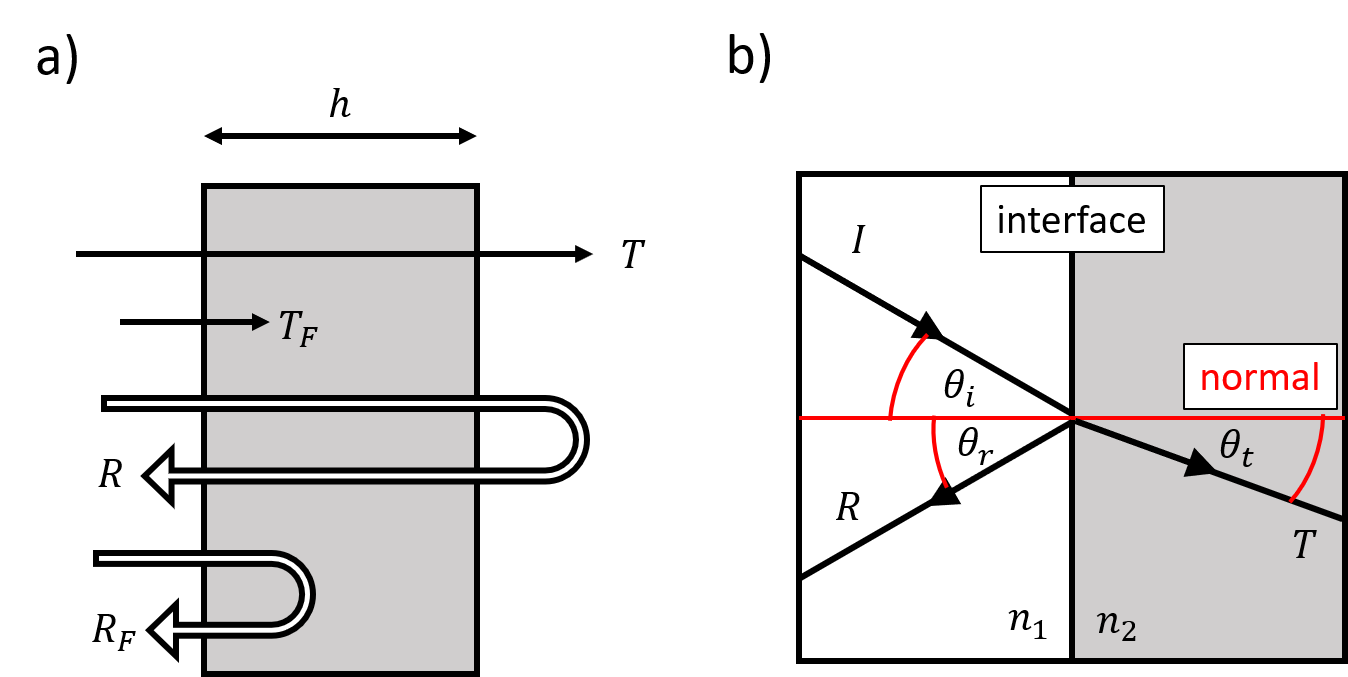
\includegraphics[width=0.75\textwidth]{figures/chap3/Fresnel_Geometry.png}
	\caption{Normal and non-normal incident geometries. \textbf{a)} Normal incidence geometry showing Fresnel coefficients $R_F$, $T_F$ for interfaces and total transmission $T$ and reflectance $R$ for a slab of thickness $h$. Figure recreated from \cite{nichelattiComplexRefractiveIndex2002}. \textbf{b)} Non-normal geometry showing definitions of angles $\theta_i, \theta_r$ and $\theta_t$ with respect to each interface.}
	\label{fig:Fresnel_Geometry}
\end{figure}

\begin{figure}
	\centering
	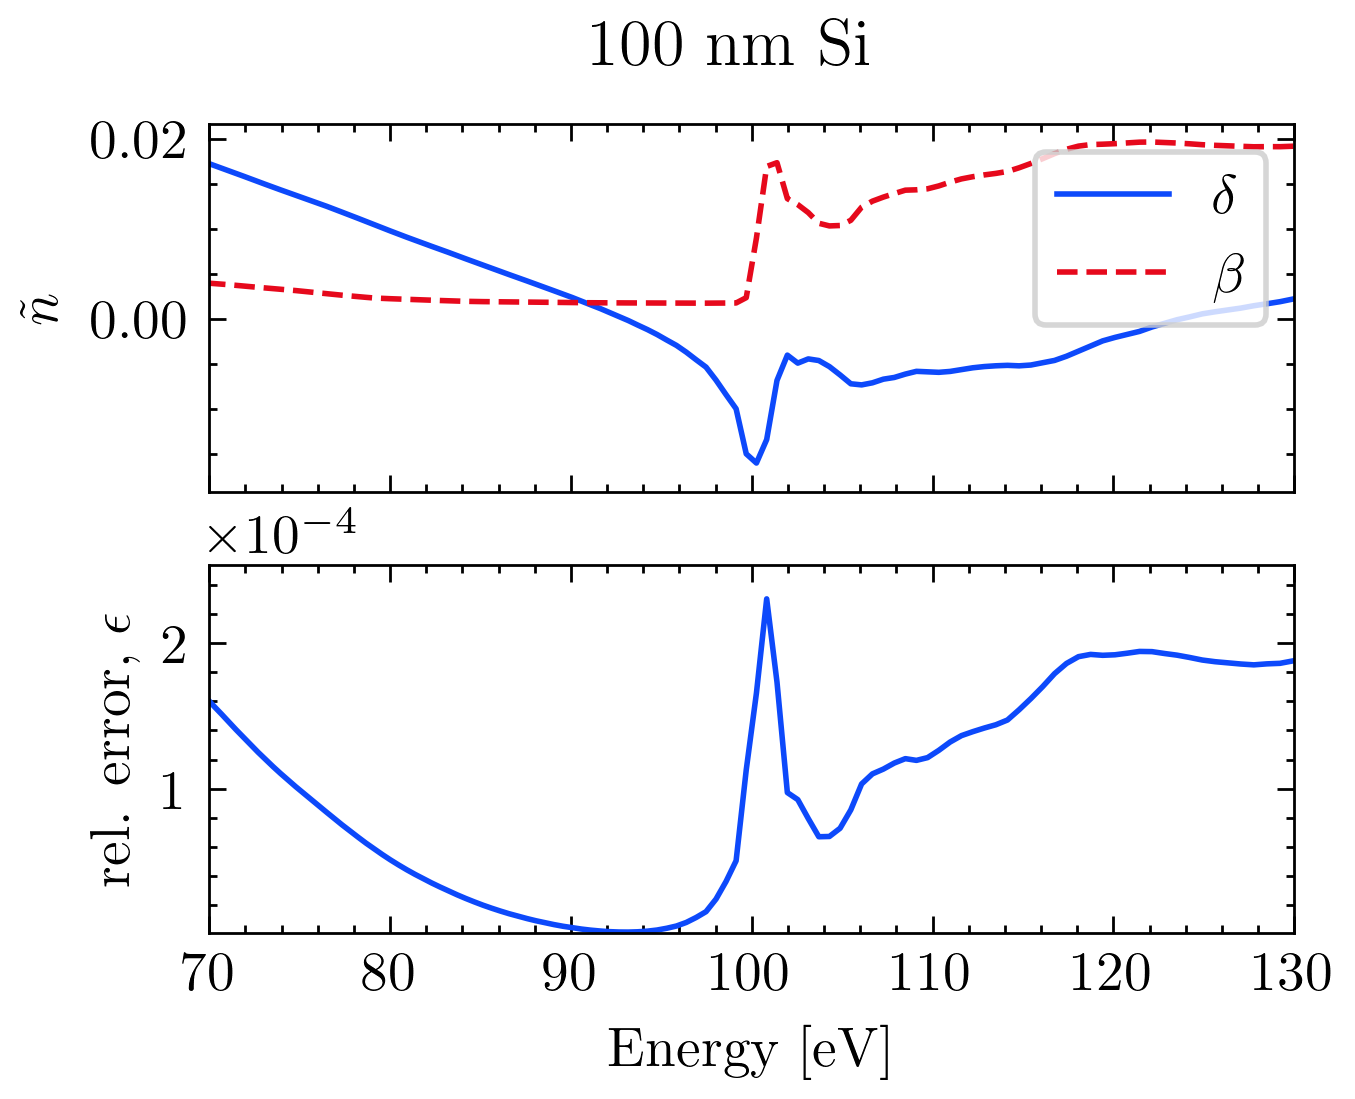
\includegraphics[width=0.75\textwidth]{figures/chap3/Si_transmission_Fresnel.png}
	\caption{Consequences of ignoring the real part of $\tilde{n}$ when calculating the transmission $T$ of a thin sample. Top panel: complex refractive index of silicon using the notation from \cref{eqn:complex_index}. The Si $L$-edge absorption feature is visible near 100 eV. Data from \cite{gulliksonCXROXRayInteractions}. Bottom panel: relative error in $T$, as defined in \cref{eqn:Fresnel_rel_err}, introduced by ignoring the contribution of $\Re(\tilde{n})$. An infinite number of bounces (e.g., \cref{eqn:Fresnel_coefs_inf_bounce}) is assumed.}
	\label{fig:Si_transmission_Fresnel}
	% plotted using \Python Scripts\CXRO\test real_imag_index_plotting.py
\end{figure}

In a transient absorption experiment, we measure the transmission $T$. Generally speaking, $T$ depends on both parts of the complex refractive index: $\tilde{n} = n + i k$. However, in a normal transmission geometry it turns out that the contribution of $\Im(\tilde{n})$ dominates the measured signal, and to a good approximation the role of $\Re(\tilde{n})$ can be ignored. Note that in a non-normal reflection geometry, both parts of $\tilde{n}$ make significant contributitions to the measured signal. In the following discussion we will analyze the Fresnel equations to see why this is the case. This section will draw from arguments made in reference \cite{nichelattiComplexRefractiveIndex2002}.

First, we consider the normal geometry shown in the left panel of \cref{fig:Fresnel_Geometry}. We write the complex index of refraction in the following form:
\begin{equation}
\begin{aligned}
\tilde{n} &= n - i k \\
&= (1-\delta) - i \beta
\end{aligned}
\label{eqn:complex_index}
\end{equation}
The Fresnel coefficients $R_F$ and $T_F$ describe the interface reflectance and transmittance and depend on both parts of the complex index $\tilde{n}$. For normal incidence, they are:
\begin{equation}
\begin{aligned}
R_F &= \left| \frac{n-ik-1}{n-ik+1}   \right|^2 \\
T_F &=  \frac{4n}{\left|n-ik+1\right|^2}
\end{aligned}
\label{eqn:fresnel_normal}
\end{equation}
Absorption in the bulk is described via the absorption length $\alpha$:
\begin{equation}
\alpha = 4 \pi k / \lambda
\end{equation}
Ignoring interface effects, the transmisison through the bulk is:
\begin{equation}
T_{\text{bulk}} = \exp( - \alpha h)
\end{equation}
Note that $\alpha$ and $T_{\text{bulk}}$ only depend on $k$.

The total reflectance $R$ and transmission $T$ are the result of interface effects plus bulk effects. We must consider the case where the detected light is the result of multiple reflections within the sample. Neglecting interference, we consider the case of $2N$ bounces where the laser's coherence length is less than the thickness of the bulk. In this case, the sum is incoherent with the expressions for $T$ and $R$ given by:
\begin{equation}
\begin{aligned}
R &= R_F + R_F T_F^2 T_{\text{bulk}}^2 \sum_{m=0}^{N} \left[ R_F T_{\text{bulk}} \right]^{2m} \\
T &= T_F^2 T_{\text{bulk}} \sum_{m=0}^{N} \left[ R_F T_{\text{bulk}} \right]^{2m}
\end{aligned}
\label{eqn:Fresnel_coefs_N_bounce}
\end{equation}
For the case of an infinite number of bounces, \cref{eqn:Fresnel_coefs_N_bounce} simplifies to:
\begin{equation}
\begin{aligned}
R &= R_F + \frac{R_F T_F^2 T_{\text{bulk}}^2}{1-R_F^2 T_{\text{bulk}}^2} \\
T &= \frac{T_F^2 T_{\text{bulk}}}{1-R_F^2 T_{\text{bulk}}^2},
\end{aligned}
\label{eqn:Fresnel_coefs_inf_bounce}
\end{equation}
whereas if only a single bounce occurs, \cref{eqn:Fresnel_coefs_N_bounce} reduces to:
\begin{equation}
\begin{aligned}
R &= R_F + R_F T_F^2 T_{\text{bulk}}^2 \\
T &= T_F^2 T_{\text{bulk}}
\end{aligned}
\label{eqn:Fresnel_coefs_1_bounce}
\end{equation}

We now consider the fractional error introduced by ignoring the interface effects described by $T_F$ and $R_F$. That is, what would happen if we assume that the interfaces have no effect on the transmitted intensity? We introduce the relative error $\epsilon$ made by ignoring the Fresnel coefficients of \cref{eqn:Fresnel_coefs_inf_bounce}:
\begin{equation}
\epsilon \equiv \frac{T_{\text{bulk}}}{T} - 1
\label{eqn:Fresnel_rel_err}
\end{equation}

As an example, consider a 100 nm thick Si sample measured in transmission near the Si $L$-edge (about 100 eV), as shown in \cref{fig:Si_transmission_Fresnel}. The relative error is in the range of one part in $10^4$ to $10^5$, well below our experimental detection limit. Silicon was chosen due to its data availability above and below the absorption edge, but this behavior is true for all materials in normal transmission.

The real part of the complex index becomes important when the sample isn't normal to the beam, as shown in the right panel of \cref{fig:Fresnel_Geometry}. In this case, the Fresnel equations are a bit messier:
\begin{equation}
\begin{aligned}
R_s &= \left| \frac{\tilde{n}_1 \cos \theta_i - \tilde{n}_2 \cos \theta_t}{\tilde{n}_1 \cos \theta_i + \tilde{n}_2 \cos \theta_t}  \right|^2 \\
R_p &= \left| \frac{\tilde{n}_1 \cos \theta_t - \tilde{n}_2 \cos \theta_i}{\tilde{n}_1 \cos \theta_t + \tilde{n}_2 \cos \theta_i}  \right|^2 \\
T_s &= 1 - R_s \\
T_p &= 1 - R_p \\
%\theta_t &= \sqrt{1- \left( \frac{n_1}{n_2} \sin \theta_i \right)^2}
\end{aligned}
\label{eqn:Fresnel_nonnormal}
\end{equation}

Here, the subscripts $s$ and $p$ denote the polarization relative to the surface normal. In a vacuum, $\tilde{n}_1=1$ and $\tilde{n}_2$ is the index of the sample. We can extract the relevant physics without any additional manipulation of the \cref{eqn:Fresnel_nonnormal}. Right away, we can see that unlike \cref{eqn:fresnel_normal}, \cref{eqn:Fresnel_nonnormal} is symmetric in the real and imaginary parts of the sample's complex index, $\tilde{n}_2$. In the limit of a thick slab, ($h \gg \alpha$), the light is attenuated before it can reflect off the back surface and we have $T \rightarrow 0$ and $R \rightarrow R_{s,p}$. That is, the only contributions to the reflected intensity are from the interface and possibly the sample volume within $z \approx 1/\alpha$ of the interface. As a result, both parts of $\tilde{n}_2$ will make significant contributions to the reflected intensity.

\section{Sample Requirements and Geometry}

\begin{figure}
	\centering
	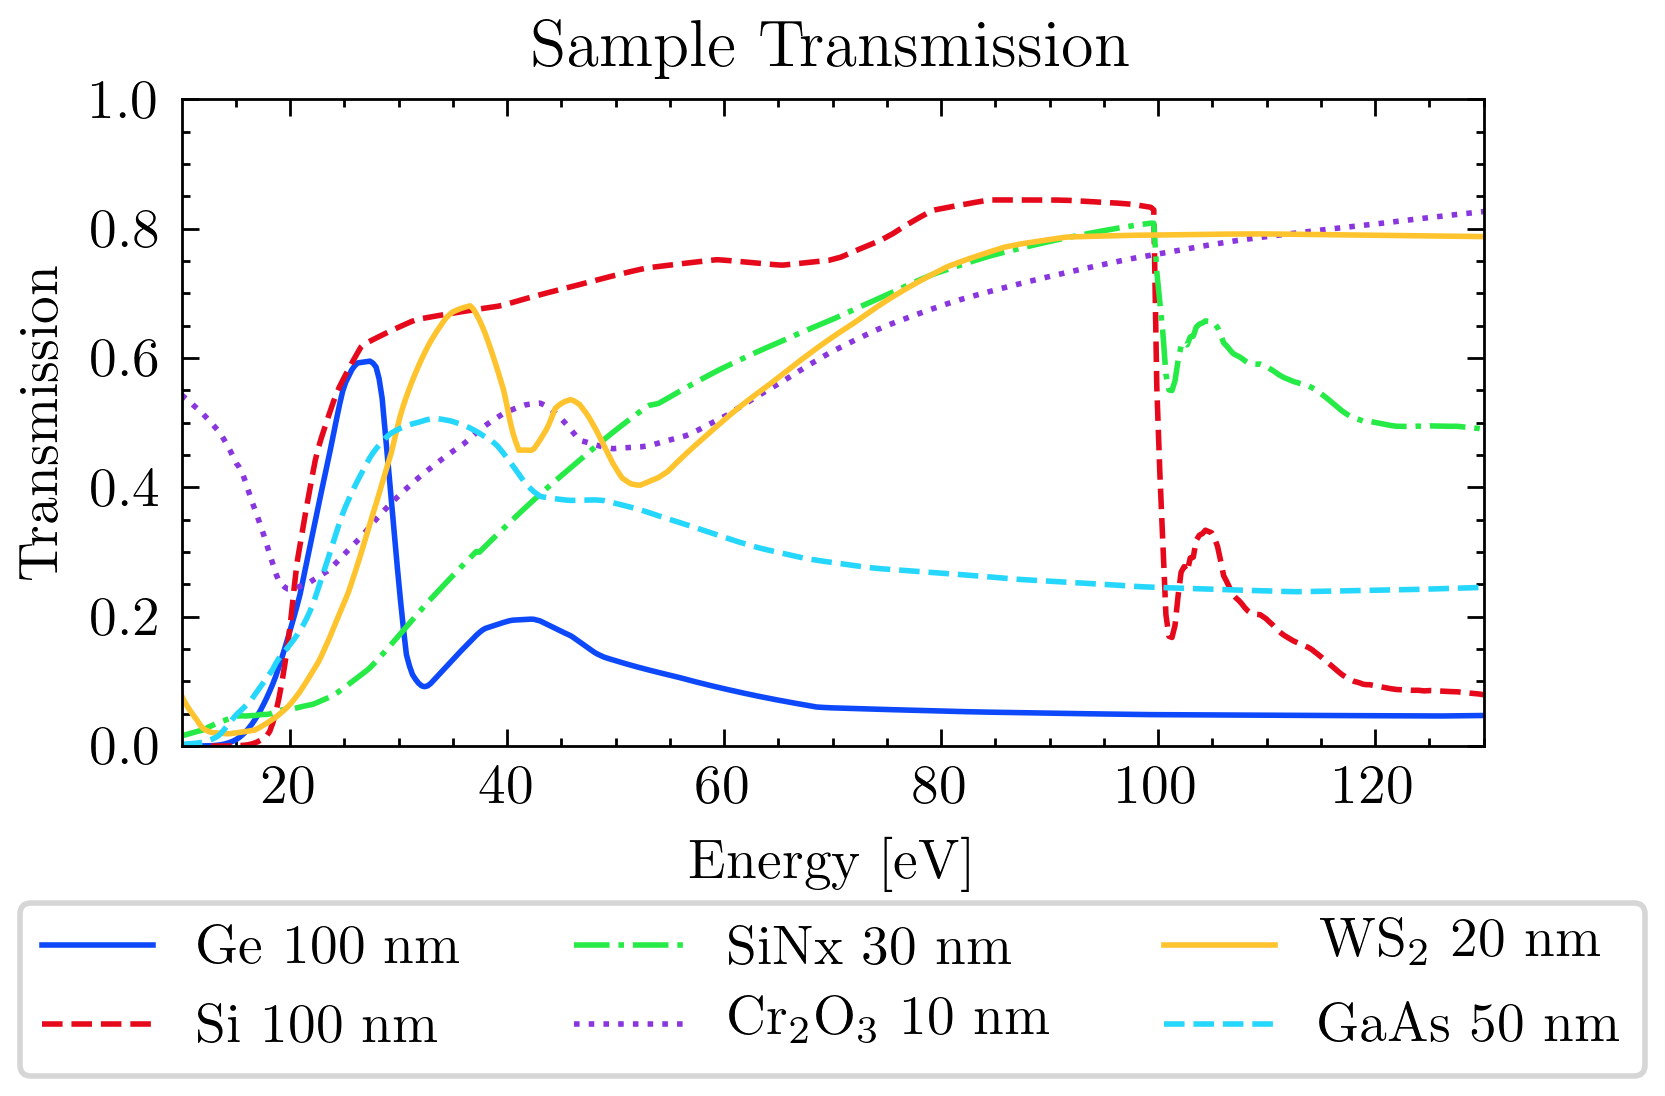
\includegraphics[width=0.75\textwidth]{figures/chap3/Sample_trans_CXRO.png}
	\caption{Calculated XUV transmission of various materials. Data from \cite{gulliksonCXROXRayInteractions}.}
	\label{fig:Sample_trans_CXRO}
	% figure generated using \PythonScripts\CXRO\test\CXRO.py
\end{figure}

There are several sample requirements for a successful condensed matter transient absorption experiment. First and foremost, the sample needs to have an absorption edge within the bandwidth of the XUV source. Second, the material must be the correct thickness for a transmission measurement, given the signal to noise of the appratus. If the material is too thick, the ground state will absorb most of the XUV flux and the resulting spectrum will be too close to the noise floor of the apparatus. If it is too thin, the laser-induced change of the ground state (on the order of $1-10\%$) will be lost in the noise. As a general guideline, a sample that absorbs 50\% at the spectral feature of interest provides a good compromise between these conflicting requirements. \cref{fig:Sample_trans_CXRO} plots the expected transmission of several materials, calculated from the atomic scattering factors \cite{gulliksonCXROXRayInteractions}. A typical sample will be on the order of 10 - 200 nm thick, depending on the material.

Another upper bound for sample thickness comes from material dispersion. In any material, the XUV light ($n_{\text{IR}} \sim 1$) will outpace the IR light ($n_{\text{IR}} > 1$). This effect can be significant if the sample is thick enough. In order to keep the phase slippage between the XUV and IR light below half an IR period, the sample thickness $h$ must obey the following relationship:
\begin{equation}
h \le \frac{1}{2} \frac{\lambda_{\text{IR}}}{n_{\text{IR}} - n_{\text{XUV}}}
\end{equation}
For germanium at $\lambda_{\text{IR}}$ = 1430 nm and probed with 30 eV XUV at $M_{4,5}$ edge at 30 eV, $n_{\text{IR}}$ = 4.2481 \cite{nunleyOpticalConstantsGermanium2016} and $n_{\text{XUV}}$ = 0.992536 \cite{gulliksonCXROXRayInteractions}, which gives a maximum thickness of 220 nm.

Next, the sample needs to be excitable using laser sources present in our lab (i.e., ultrafast pulses with wavelengths between 800 nm and a couple of microns). To minimize the slow build up of heat (on the order of seconds) and laser-induced damage, the sample needs to be rastered through the laser focus as the experiment is performed. This rastering method necessitates both a large clear aperture ($\sim$ 1 mm$^2$ - 1 cm$^2$) and good sample uniformity. Samples that meet the above thickness and clear aperture requirements are extremely delicate, with thicknesses between 5,000 and 100,000 times smaller than their freestanding lateral dimensions. As such, one should expect most samples to break before, during and after measurements, and a successful experiment will have a materials pipeline that is capable of producing multiple, consistent samples in a short time frame.

\section{Absorbance and Transient Absorbance Data Collection Methods}

\begin{figure}
	\centering
	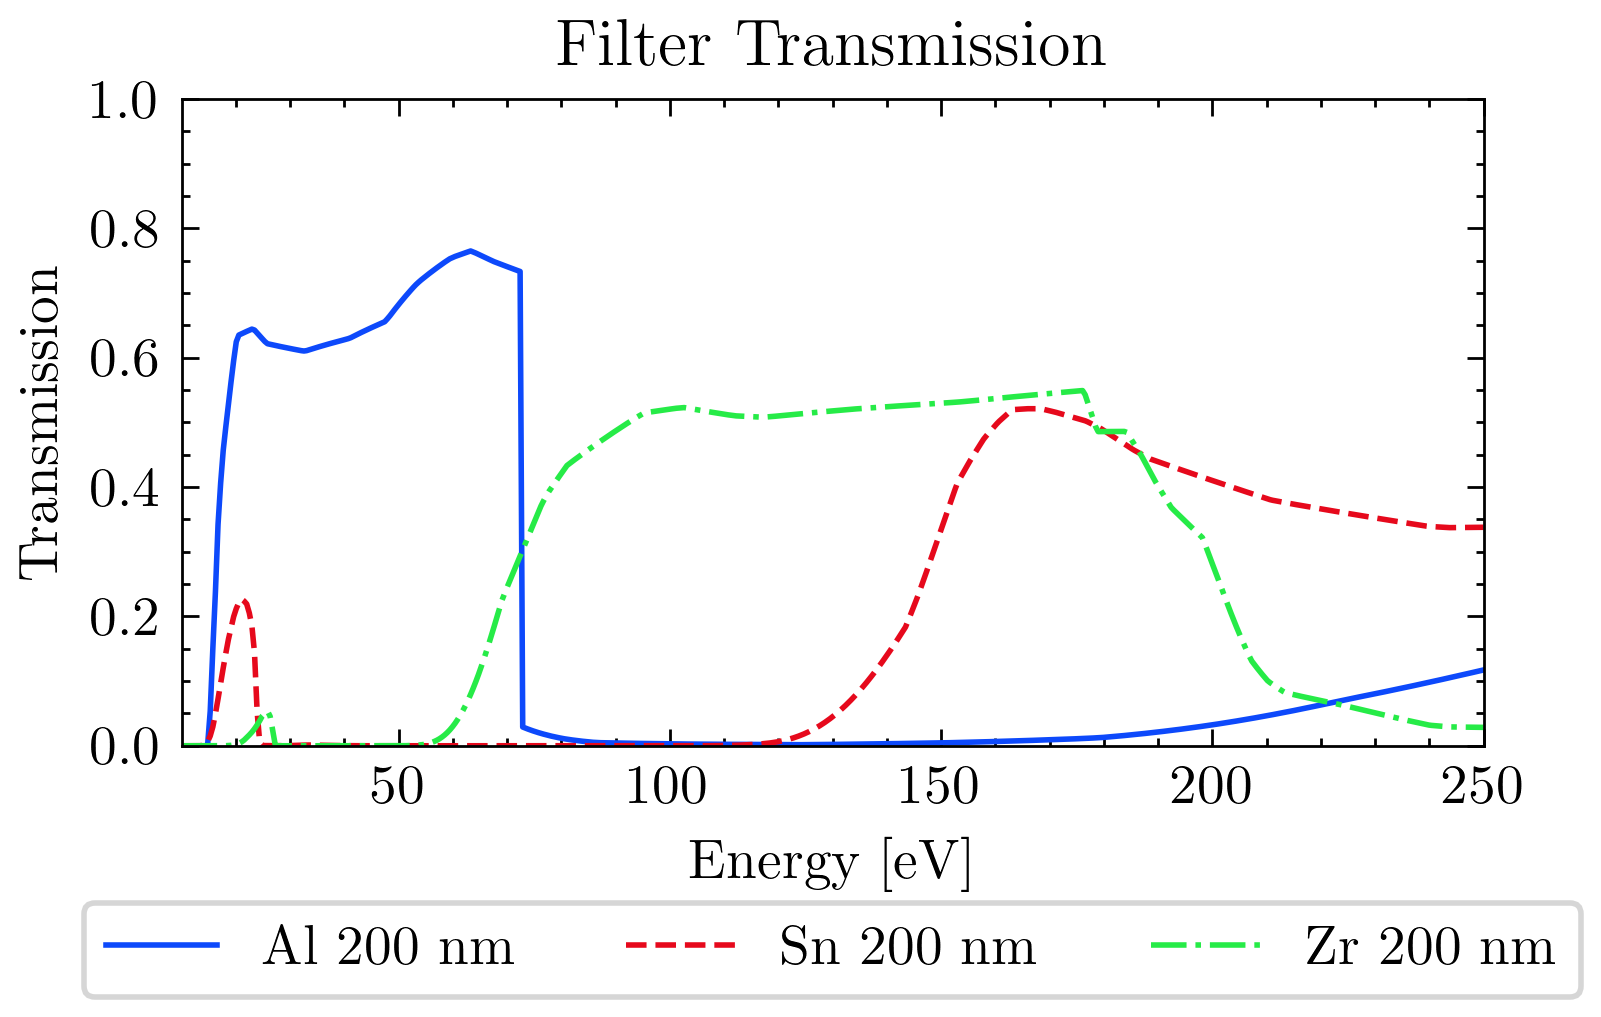
\includegraphics[width=0.75\textwidth]{figures/chap3/Filter_transmission_CXRO.png}
	\caption{Calculated XUV transmission of various metallic filters. Data from \cite{gulliksonCXROXRayInteractions}.}
	\label{fig:Filter_transmission_CXRO}
	% figure generated using \PythonScripts\CXRO\test\CXRO.py
\end{figure}

\begin{figure}
	\centering
	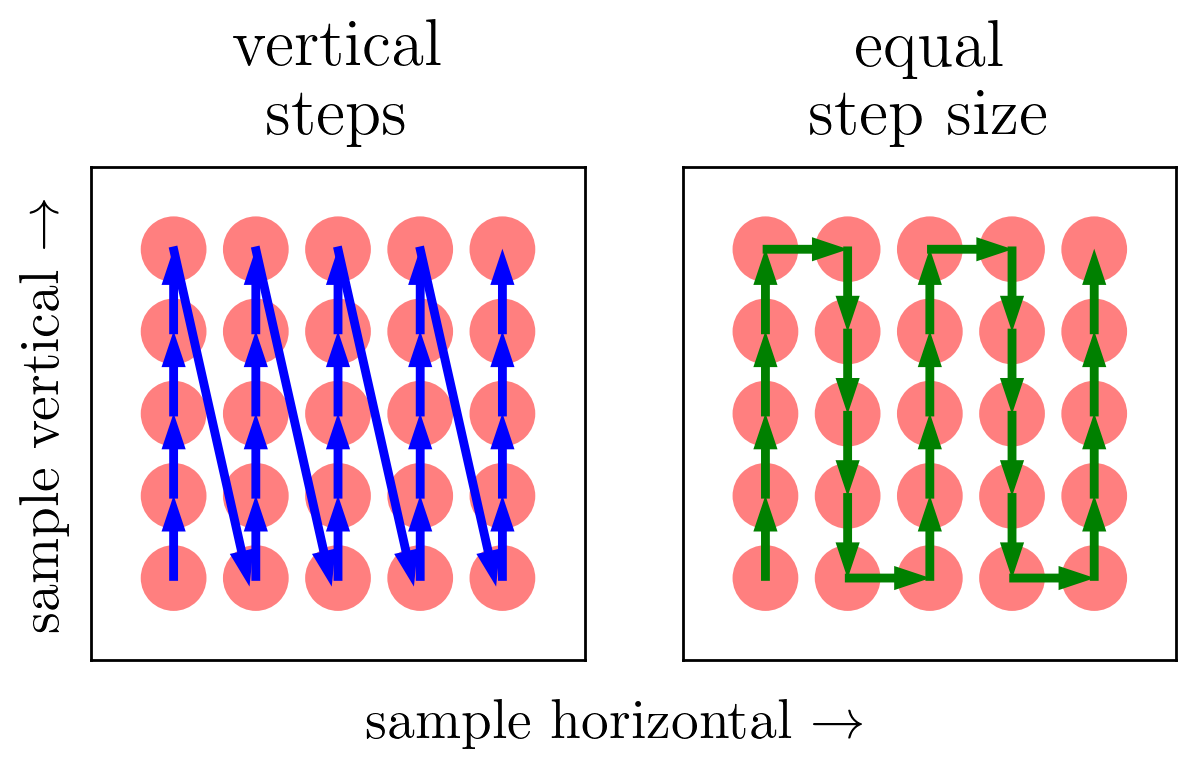
\includegraphics[width=0.75\textwidth]{figures/chap3/Rastering_Methods.png}
	\caption{Schematic of competing raster methods, shown in the sample's reference frame. The clear aperture of the sample is represented by the interior of the black square. The laser propagation direction is out of the page. The laser focal spots are shown as red circles, and the movement of the sample holder relative to the laser focus is indicated by arrows. This diagram is to scale for a $1\times1$ mm$^2$ clear aperture sample, a 60 $\mu$m diameter IR focal spot and a 200 $\mu$m step size.}
	\label{fig:Rastering_Methods}
	%figure created using \Python Scripts\rastering\raster_diagram.py
\end{figure}

\begin{figure}
	\centering
	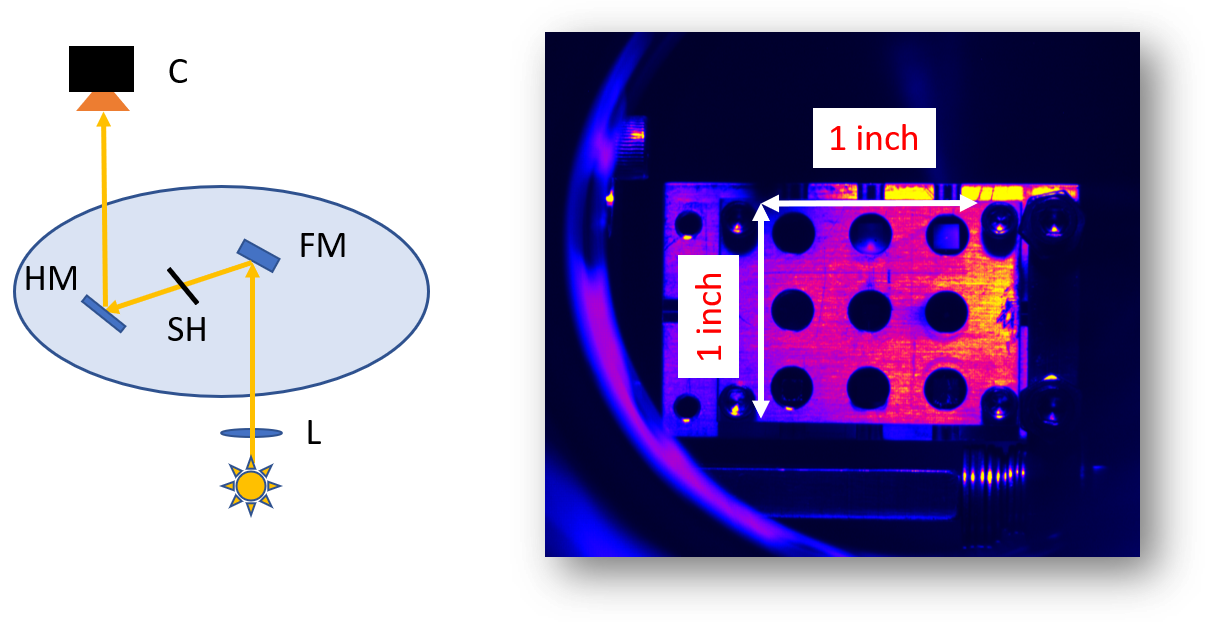
\includegraphics[width=0.75\textwidth]{figures/chap3/sample_holder.png}
	\caption{\textit{In-situ} imaging of the samples within the target chamber. Left: optical setup for \textit{in-situ} imaging of samples. C: Si CCD camera, HM: hole mirror, SH: sample holder, FM: flip mirror, L: lens. Right: false color image showing the sample holder with a 3 x 3 grid of 5 mm diameter clear apertures. Samples are held in a clamshell design centered in the clear apertures. Samples are backlit using a flashlight.}
	\label{fig:sample_holder}
\end{figure}

The \textit{absorbance}\footnote{The terms absorbance and optical density are often used interchangably.} $A$ is defined as the negative logarithm of the transmission $T$:
\begin{equation}
A(E) = -\log_{10} \left( T \right) = -\log_{10} \left(\frac{S_{gs}(E)}{S_{vac}(E)} \right).
\label{eqn:absorbance}
\end{equation}

In \cref{eqn:absorbance}, $S_{gs}(E)$ is the XUV spectrum transmitted by the sample in its ground state and $S_{vac}(E)$ is the spectrum without the sample present. Therefore we can measure the sample's ground state absorbance by measuring the harmonic spectrum with and without the sample in the XUV beam.

The \textit{change in absorbance} $\Delta A$ between the ground and excited state which is induced by an IR pulse is therefore:
\begin{equation}
\begin{aligned}
\Delta A(E,\tau) = & A_{\text{sig}}(E,\tau) - A_{\text{gs}}(E) \\
= & -\log_{10} \left(\frac{S_{\text{sig}}(E,\tau)}{S_{\text{vac}}(E)} \right) -  \log_{10} \left(\frac{S_{\text{gs}}(E)}{S_{\text{vac}}(E)} \right) \\
= & -\log_{10} \left(\frac{S_{\text{sig}}(E,\tau)}{S_{\text{gs}}(E)} \right).
%\Delta A(E,\tau) = -\log_{10} \left(\frac{S_{sig}(E,\tau)}{S_{gs}(E)} \right).
%\label{eqn:delta-OD}
\end{aligned}
\label{eqn:delta-A}
\end{equation}
In \cref{eqn:delta-A}, the signal spectrum $S_{\text{sig}}(E,\tau)$ is the spectra that results from an IR pulse hitting the sample, followed by an XUV pulse after a delay of $\tau \equiv t_{\text{XUV}} - t_{\text{IR}}$. Note that negative delays mean the XUV arrives at the sample before the IR and zero delay indicates temporal overlap of the two pulses. It is assumed that a delay of negative infinity is equivalent to a ground state measurement: $S_{\text{sig}}(E,\tau=-\infty) = S_{\text{gs}}$.

An ATAS experiment is simply a collection of recorded spectra taken over a range of delay points with otherwise identical experimental conditions. However, we have implemented several techniques to improve the fidelity of our data.

HHG is an extremely inefficient process, with a conversion ratio on the order of $10^{-6}$. After the generation cell, the leftover IR light must be blocked or it will destroy any sample located downstream. We use a thin metallic filter (Al, Zr or Sn), placed about 1 m after the harmonic source, to strip out the generating infrared field. The choice of filter is dictated by the photon energy range of the spectral features we want to study. For more detail, see \cref{fig:Filter_transmission_CXRO}.

As an extremely nonlinear process, HHG's conversion efficiency is highly dependent on the input laser pointing, peak power, pulse duration, spatial mode, etc. -- all of which are affected by laboratory environmental conditions and the activity of other group members within our lab complex. As a result, even during ``ideal'' experimental conditions, the total harmonic yield drifts slowly throughout the course of the experiment. To minimize the effect of this slow drift, we take a ground state spectrum for each delay point. A computer-controlled home-built shutter system blocks the IR laser in the pump arm between measurements (see \cref{fig:beamline_schematic}). Taking back-to-back ground and excited state spectra significantly lowers the harmonic stability requirements; we require stability on the order of twice the exposure time (several seconds), rather than the entire experimental run (several hours).

Our spectrometer's CMOS camera has a bit depth of 16, corresponding to a maximum value of $2^{16}-1 = 65,535$ counts before saturation. The exposure time is set so that the amplitude of the brightest harmonic on the detector is about 10\% below this limit, which allows for an upward drift in harmonic yield to occur without invalidating the dataset. An exposure time of 3 seconds is typical for a 200 nm Al filter with a 100 nm Ge sample at 125 Hz (375 laser shots), an MCP voltage of 2200 VDC, and $2\times2$ camera pixel binning.

Although the Spitfire laser system has a maximum repetition rate of 1 kHz, we perform solid state ATAS experiments at a much lower rate (125 or 250 Hz) by adjusting amplifier's Pockels cell firing rate. The lower repetition rate allows the sample to more fully relax between laser shots, reducing the effects of millisecond thermal processes on our measurements. It also reduces the average power on the sample for a given pulse energy, which lowers the steady state temperature of the sample. On the other hand, it allows us to increase the pulse energy while maintaining a constant average power on the sample.

During the experiment, the sample is rastered across the focus to reduce any deleterious effects of long term uninterrupted laser exposure. During motor movement, the IR beam is blocked with a shutter but the relatively weak XUV beam is allowed to remain on the sample. Each pair of measurements (ground state, excited state) in a given delay scan has a unique position on the sample. Typical step sizes are 200 $\mu$m, which is larger than the measured XUV spot size of $\sim$12 $\mu$m and the IR spot size of $\sim$30 $\mu$m. Two raster schemes are schematically shown in \cref{fig:Rastering_Methods}. The method shown in the left panel produces a sawtooth pattern on the sample. This method gives very accurate positioning, as the vertical motor is almost always approaching the final position from the same direction. However, the diagonal steps are $\sqrt{N^2+1}$ times longer than the vertical steps, where $N$ is the number of vertical steps in the pattern. As a result, there is a bimodal distribution of motor transit times between measurements. If the sample is not fully relaxed between motor movements, this will lead to an inconsistent measurement of the ground state $S_{gs}(E)$. The method shown in the right panel alleviates this problem by requiring equal step sizes. Measurements presented in this work were acquired using the method shown in the right panel.

Before measuring a sample's response for the first time, or after a major optical alignment, a map of the sample must be created. Creating this map serves two purposes: it verifies sample XUV absorption uniformity and it determines the motor coordinates of the sample's clear aperture. To avoid edge effects, the edges of the raster area are chosen to be 200 $\mu$m away from the edge of the clear aperture (see \cref{fig:Rastering_Methods}).

The next step is a measurement of the absorbance ($A$) of the ground state of the sample. This is achieved by taking spectra with ($S_{\text{gs}}$) and without ($S_{\text{vac}}$) the sample in the XUV beam. These measurements are taken back-to-back (as quickly as the motors will allow, $<$10 seconds between spectra) to minimize harmonic drift between measurements. Note that because we do not have a simultaneous harmonic amplitude reference measurement, a change in the XUV input flux during this measurement can manifest itself as a change in the absorbance. A typical ground state measurement of a 100 nm Ge sample is shown in \cref{fig:Ge_100nm_ground_state}.

The transient data collection sequence can be summarized as \textit{excited state $\rightarrow$ ground state $\rightarrow$ move motors}. Details of this sequence are as follows. First, the sample moves to a given raster position and delay wedge position, the IR shutter opens and an excited state spectrum ($S_{\text{sig}}(\tau,E)$) is recorded. Then, the IR shutter closes and a ground state spectrum ($S_{\text{gs}}(E)$) is recorded. To minimize the duration of the experiment, an XUV reference spectrum ($S_{\text{vac}}(E)$) is not recorded. Finally, the sample moves to the next raster position as the delay wedge pair moves to the next delay position. The system is programmed to wait for the wedges to become stationary before the next measurement begins.

Note that in this sequence, the time between the $i^{th}$ excited state and $i^{th}$ ground state measurements is equal to the exposure time, but the time between the $i^{th}$ ground state measurement and the $(i+1)^{th}$ excited state measurement is equal to the delay wedge motor transit time\footnote{In this analysis we neglect the role of the XUV-IR delay $\tau$. However, $\tau \sim$ 1 fs - 1 ps, which is neglible compared to the motor transit time $\sim$ 1 s.}. This sequence is preferable to the alternative (\textit{ground state $\rightarrow$ excited state $\rightarrow$ move motors}), as that would result in a delay step size-dependent relaxation time between the $i^{th}$ excited state and the $i+1^{th}$ ground state measurement. Since $\Delta A(E,\tau)$ is calculated between pairs of ground and excited state measurements at a given delay wedge position, the sequence \textit{excited state $\rightarrow$ ground state $\rightarrow$ move motors} is preferred.



To further improve our signal to noise ratio, we average multiple delay scans together. A typical $\Delta A$ measurement will repeat a delay scan between 10 and 50 times. Each delay scan uses the raster points of the previous delay scan so there is a one-to-one mapping of delay to sample position.



damage thresholds, sample thickness, sample uniformity

creating XUV sample maps when we get a new. this allows us to map out the clear aperture of the sample, as well as checking the uniformity of the sample.

\section{The Supporting Membrane}

\begin{figure}
	\centering
	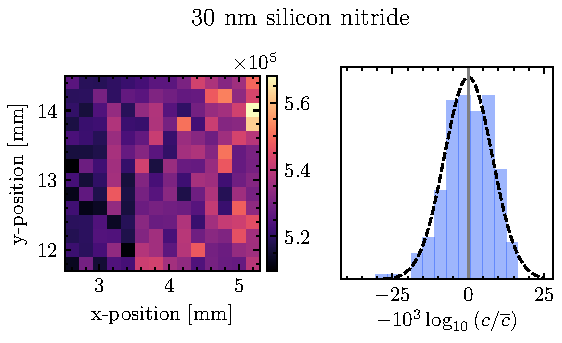
\includegraphics[width=0.75\textwidth]{figures/chap3/nitride_map.png}
	\caption{XUV transmission map of 30 nm silicone nitride freestanding membrane. Left panel: integrated harmonic peaks in the range ?? -- ?? eV. Sample holder motor positions are indicated by x- and y-positions. Right panel: histrogram of logarithmic deviation of counts from the average. Dashed line shows a normal distribution.}
	\label{fig:nitride_map}
	% figure created using \Python Scripts\Spectrometer\test\rastermap.py
	% dataset: C:\testdata\2019_09_10\4_55_32 PM_nitride_map1
\end{figure}

\begin{figure}
	\centering
	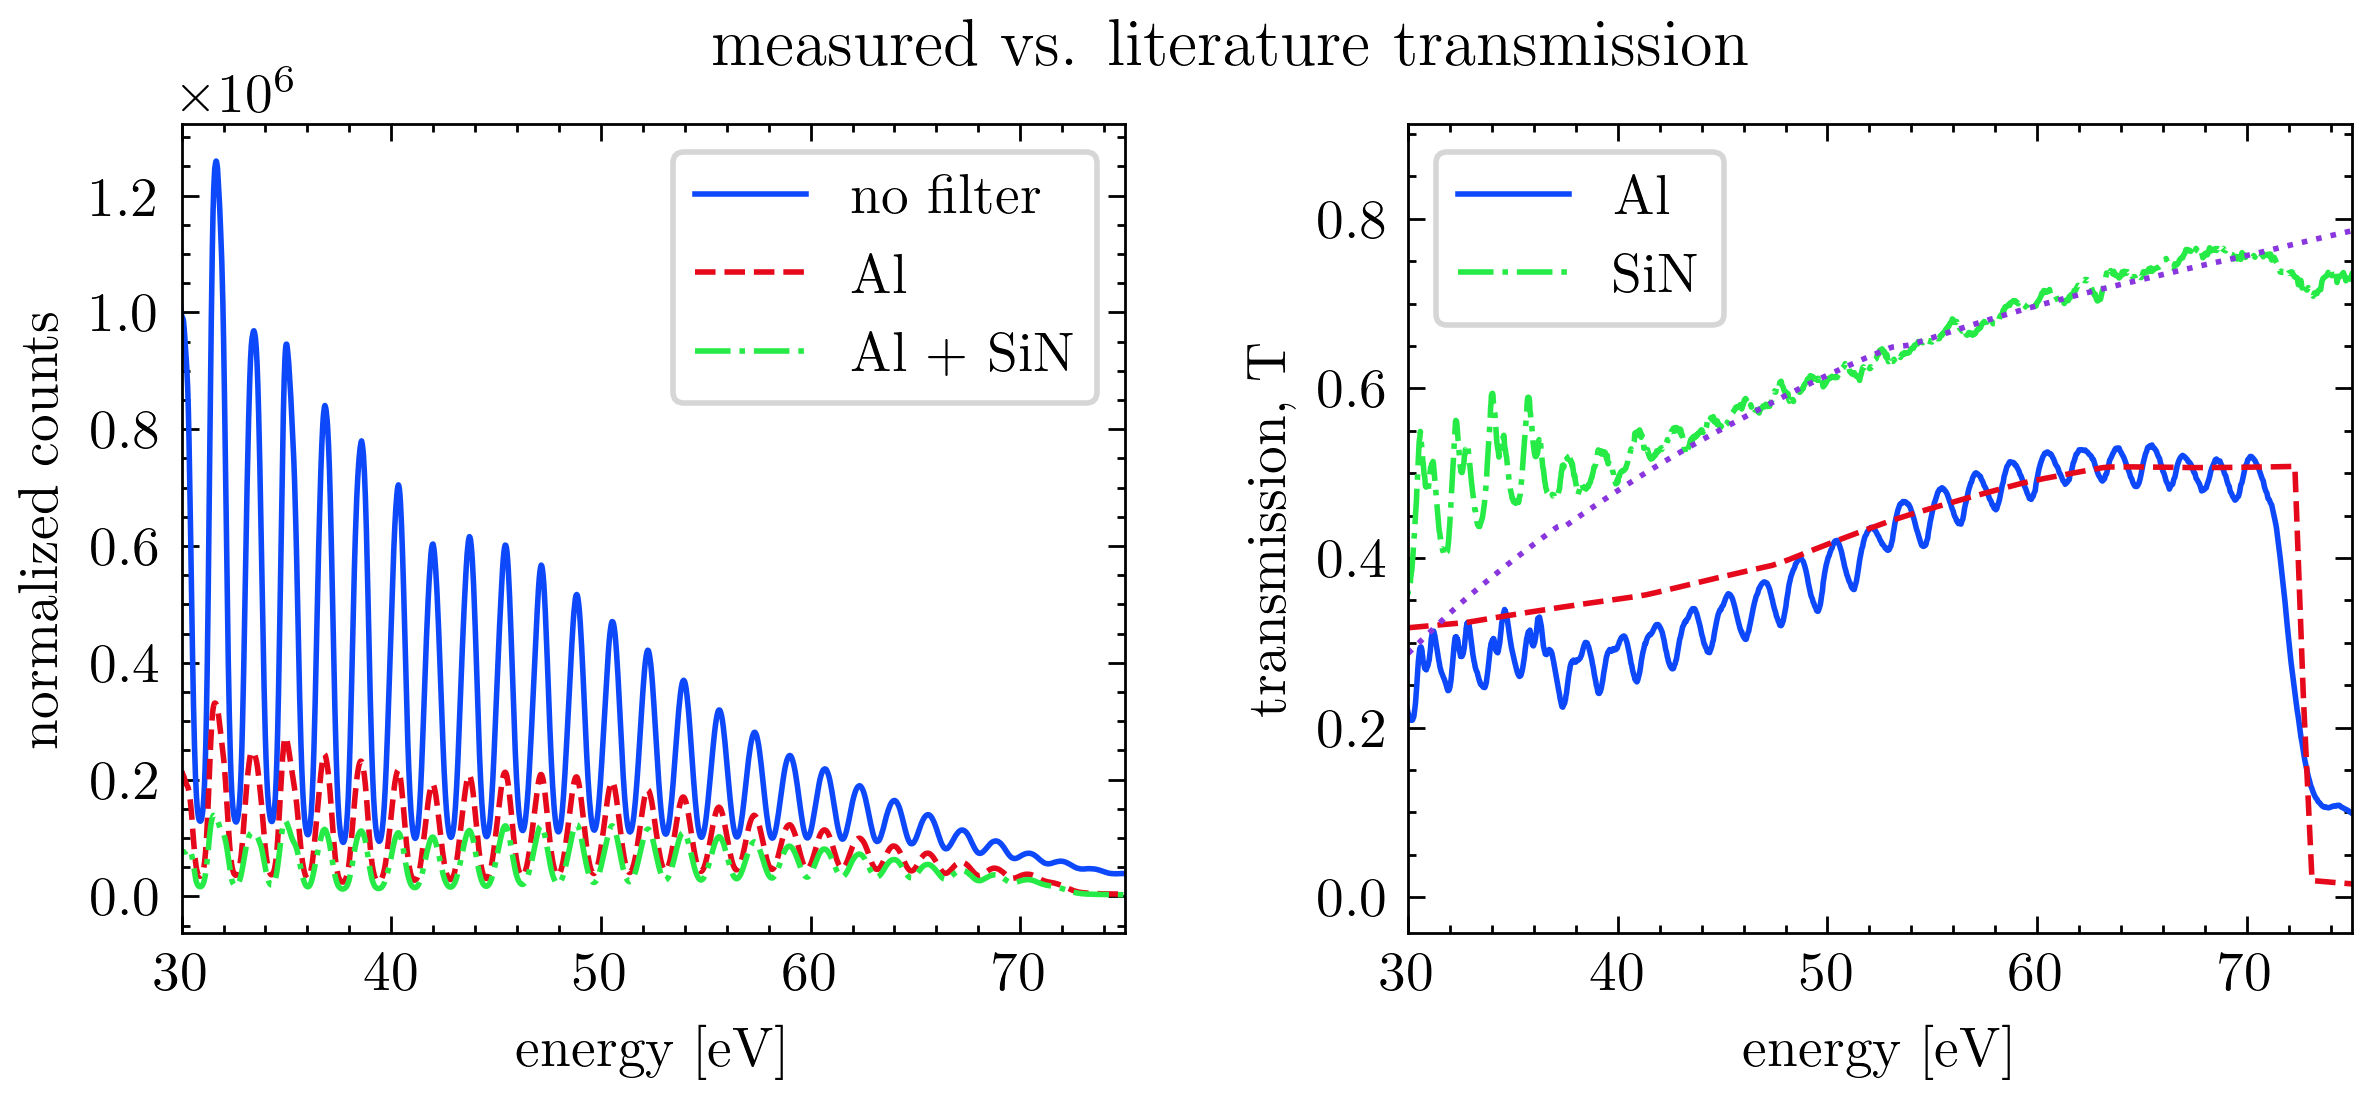
\includegraphics[width=0.75\textwidth]{figures/chap3/SiN_Al_transmission.png}
	\caption{XUV transmission measurements of Al metallica filter and silicon nitride membrane. Left panel: normalized XUV counts for i) unfiltered HHG signal, ii) HHG going through a 200 nm Al filter and iii) HHG going through a 200 nm Al filter and 30 nm of silicon nitride. Counts are scaled by the Jacobian (\cref{eqn:spectrometer_jacobian}). Right panel: transmission curves obtained from the left panel's data. Also shown are literature values for 20 nm of silicon nitride and 200 nm of Al with two 4 nm oxide layers \cite{gulliksonCXROXRayInteractions}. Multilayer interference is not taken into account. Oscillations in measured transmission are numerical artifacts which will be discussed in the text.}
	\label{fig:SiN_Al_transmission}
	% dataset: \2019_05_02\
	% plotted using: \Python Scripts\Spectrometer\test\nitride_trans.py
\end{figure}

\begin{figure}
	\centering
	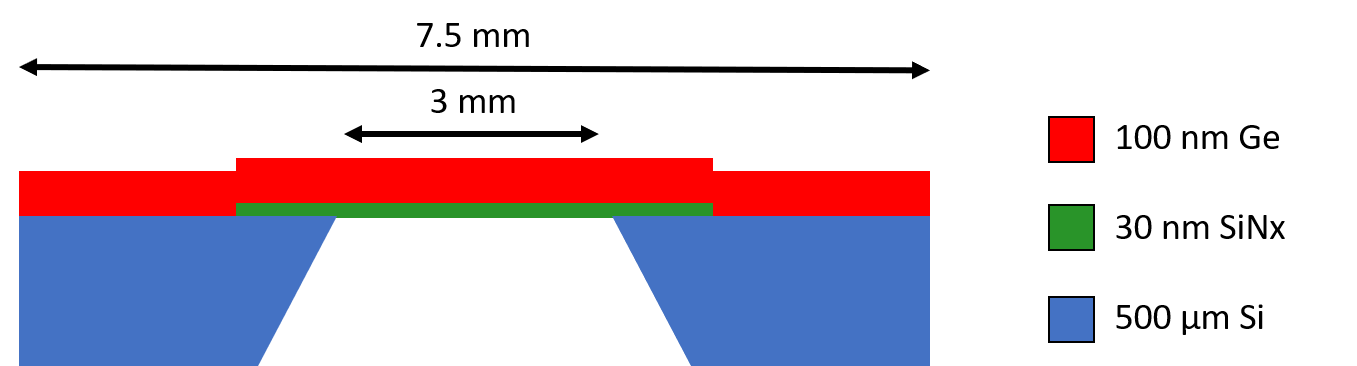
\includegraphics[width=0.75\textwidth]{figures/chap3/Sample_Geometry.png}
	\caption{Cartoon showing the cross section of the free standing sample heterostructure. A 500 $\mu$m thick Si frame supports a freestanding 30 nm low stress silicon nitride membrane (Norcada QX7300X), upon which 100 nm of germanium has been deposited. The Si frame has a 3x3 mm$^2$ square clear aperture and a 7.5x7.5 mm$^2$ square external dimension. The taper of the Si frame thickness along the perimeter of the clear aperture forms a knife edge. In an ATAS experiment, the XUV and IR pulses propagate from the top to bottom of the figure.}
	\label{fig:Sample_Geometry}
\end{figure}

While most materials have an absorption edge within the range 25 - 150 eV, there are very few commercially available pre-fabricated materials with both the requistite large clear aperture and thickness. Note that either characteristic is relatively easy to achieve individually, but their combination presents unique materials challenges. We review three synthesis methods that can produce a quasi-2D sample:
\begin{enumerate}
	\item sample growth on a traditional substrate, followed by chemical back-etching or milling of the substrate until sub-micron thickness of the heterostructure is achieved;
	\item sample growth on a traditional substrate, followed by mechanical transfer onto a membrane;
	\item sample growth on a membrane.
\end{enumerate}
Sample quality and composition is heavily impacted by local growth conditions such as substrate temperature, deposition rate, substrate crystal cut, substrate-sample lattice mismatch, etc. Many of these characteristics are changed when growing on a substrate of a different cut, or by replacing a substrate with a membrane. In general, one should not expect success when applying a substrate-optimized growth recipe to a freestanding membrane. Therefore, methods 1 and 2 will yield the highest quality samples, as they leverage already-developed sample recipes. However, both methods require a technically difficult second step that is prone to failure.

Selective chemical etching recipes exist for certain compounds, but they usually require an additional layer in the heterostructure to protect the sample. Adding this layer will come at the expense of the total XUV flux transmitted by the heterostructure. Additionally, the chemical etching rates are highly dependent on local chemistry, fluid convection and temperature \cite{chiuPhotoluminescenceEvolutionGaAs2015}, which ultimately means that the amount of material removed is uncontrollable and unrepeatable within our requirements (499.9 $\mu$m $\pm$ 10 nm removed from a 500 $\mu$m substrate). For these reasons, we decided to not pursue a chemical etch recipe. Ion or electron milling is more controllable, but too expensive to implement on a large scale. The above reasons preclude the use of Method 1.

Mechanical transfer of thin samples is a tried and true method, but it usually results in flakes with lateral dimensions on the order of 100 $\mu$m. Repeated transfer of many flakes is possible, but there little control over their exact positioning on the membrane. This results in folded or overlapping flakes. These mishaps increase the effective optical density of the sample, changing the IR and XUV absorption properties significantly.

An XUV spatial measurement needs to be taken prior to any ATAS experiment, but a non-uniform distribution of flakes on a membrane would require a much higher resolution map. This is because the flakes are on the order of the XUV and IR focii, so it is critical that the raster points in \cref{fig:Rastering_Methods} correspond to the center of each flake to avoid edge diffraction and to minimize the effects of slow laser pointing drift. For a uniform film, a map can be taken using 200-250 $\mu$m step sizes, as the most important feature is the border of the clear aperture. On the other hand, each flake would have to be sampled $\sim$5 times in each direction to find its center. As a conservative estimate, a membrane covered with $100 \times 100\text{ }\mu$m$^2$ flakes would require a step size of 20 $\mu$m, which increases the number of raster points by a factor of $10^2 = 100$. Considering that a $3 \times 3 \text{ mm}^2$ clear aperture sampled with 200 $\mu$m steps takes $\sim$45 minutes to map, a random distribution of flakes would take a prohibitively long time to map out.

With the first two methods ruled out, we turn to the third method of growing directly on a freestanding membrane. Although it will result in a lower quality sample, it does not have the same technical hurdles of the previous two methods. However, the large clear area makes the heterostructure extremely fragile. We initially attempted to circumvent this problem by using smaller clear apertures.

As shown in \cref{fig:Rastering_Methods}, most of the sample's area isn't directly used by the laser - it exists as a buffer between the grid of sample points. An alternative to a single clear aperture is an array of micro-apertures, each with a diameter on the order of the IR spot size. The micro-apertures exist within a mechanically robust substrate and a thin membrane lies on top of the structure. This configuration significantly eases the material strength requirements by reducing the size of the unsupported area from cm-scale to sub-mm-scale. The regular grid of apertures avoids the difficulties of a randomly distributed sample, easing the XUV mapping step size requirements. Fortunately, these arrays are commercially available from Silson, Norcada (silicon nitride membranes) and US Applied Diamond (diamond membranes) but we encountered technical difficulties in their implementation. Because the aperture size is on the order of the size of the IR focal spot, there is very little room for positioning error, and our motors were insufficiently precise for this application. Further, these arrays are typically only available in at most a $3\times3$ array, which provides an insufficient number of raster points for an experiment.

With these limitations in mind, we decided to use large aperture x-ray windows from Norcada. These windows consist of a mechanically robust Si frame substrate with a square clear aperture cut through the center. The structure is fabricated so that a thin membrane covers the clear aperture. A cross section is shown in \cref{fig:Sample_Geometry}.

Norcada offers these structures with either a silicon (polycrystalline or single-crystal) or a silicon nitride membrane. An ideal membrane is transparent to both XUV and IR wavelengths with a high damage threshold. Referring to \cref{fig:Sample_trans_CXRO}, 100 nm of Si provides a relatively flat transmission curve from 25 to 100 eV. In constrast, 30 nm of silicon nitride has poor, but featureless, transmission at lower energies. Both materials transmit light below their bandgaps (5 eV for SiN and 1.14 eV for Si). Finally, silicon nitride's higher bandgap results in a significantly higher laser damage threshold \cite{gamalyAblationSolidsFemtosecond2002, austinFemtosecondLaserDamage2018, keldyshIonizationFieldStrong1965}. Taking all these factors into account, we decided to use 30 nm silicon nitride membranes for germanium transient absorption experiments. The measured transmission of a typical membrane is shown in \cref{fig:SiN_Al_transmission}.

Likewise, experiments with micro-flakes of $WS_2$ samples were attempted, 



\section{Germanium as a Sample}

\begin{figure}
	\centering
	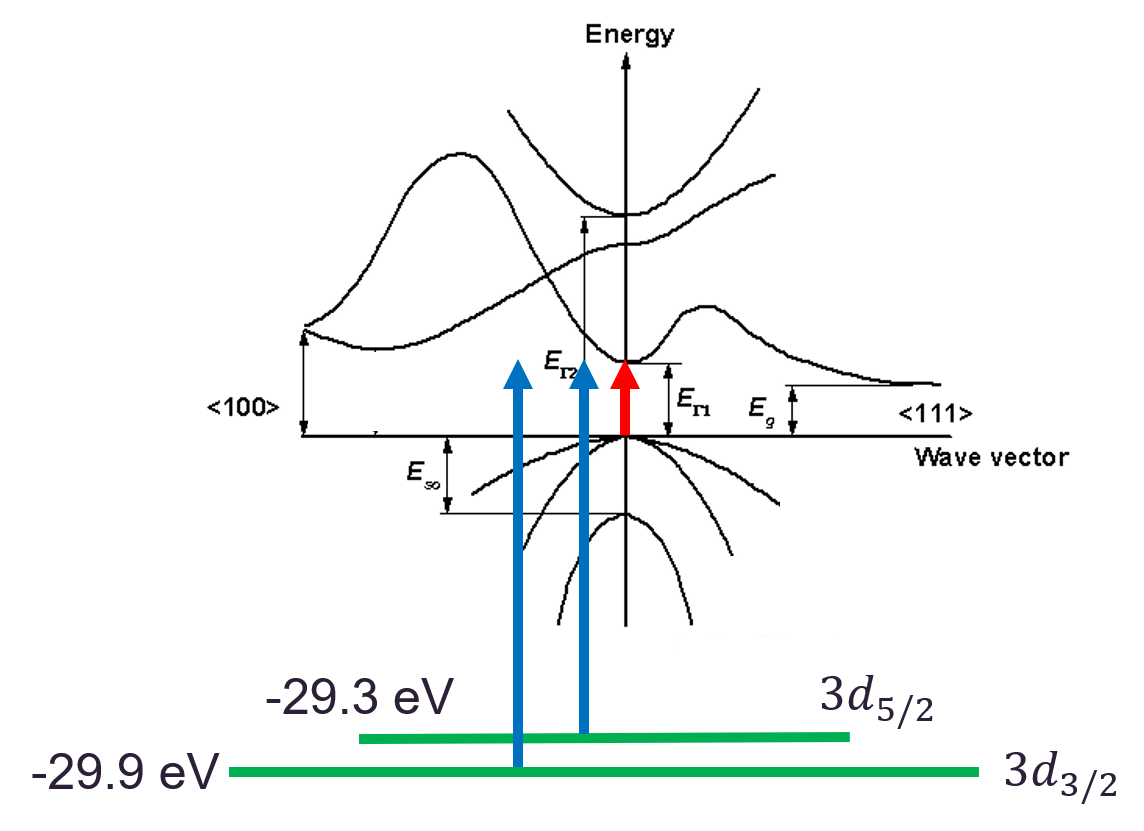
\includegraphics[width=0.5\textwidth]{figures/chap3/Ge_band_diagram.png}
	\caption{Band structure and $3d$ states of Germanium. Blue arrows indicate XUV-induced transitions from the core levels to valence and conduction bands. Red arrows indicate IR-induced transitions across the band gap. Arrows are displaced horizontally for visual clarity. Figure adapted from \cite{NSMArchivePhysical}.}
	\label{fig:Ge_band_diagram}
\end{figure}

\begin{figure}
	\centering
	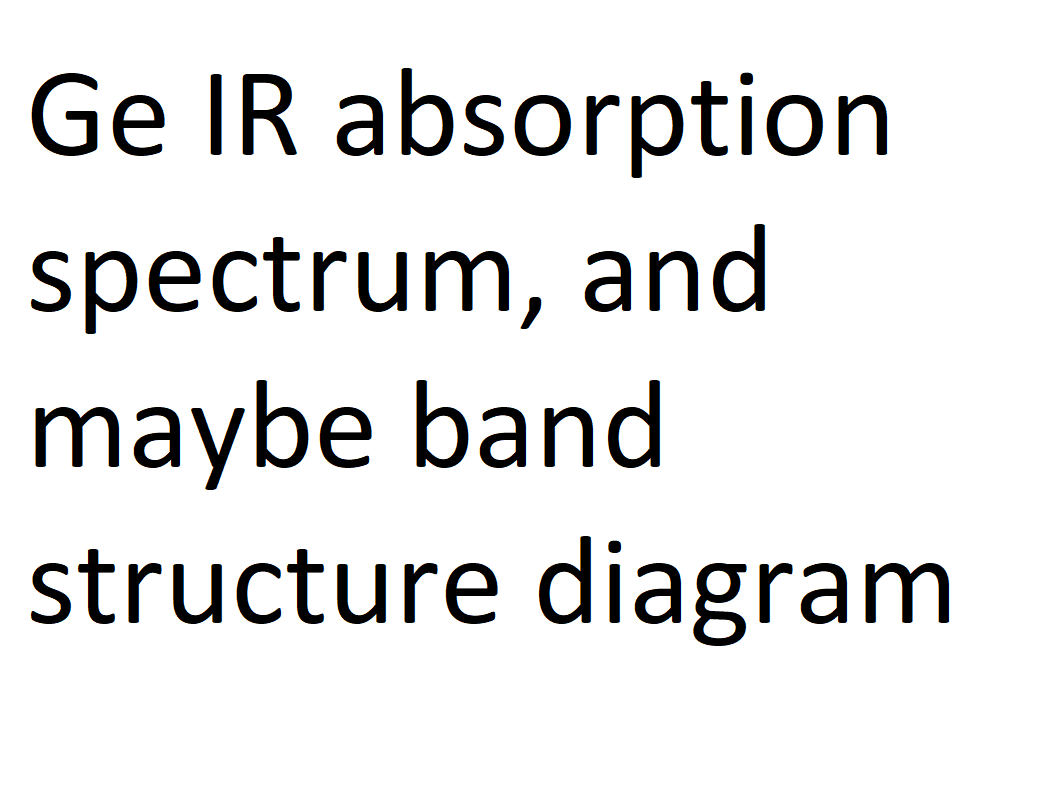
\includegraphics[width=0.5\textwidth]{figures/chap3/Ge_IR_absorption.png}
	\caption{this figure shows the IR absorption of germanium from the literature. (citation). or maybe the n,k values from refractiveindex.info}
	\label{fig:Ge_IR_absorption}
\end{figure}

talk about the germanium sample, why it was chosen as a sample, how it was grown and how thick it was.



\section{IR Pump Arm Considerations}


In a condensed matter ATAS measurement, the IR intensity is usually set to be as high as possible (while avoiding sample damage) to maximize the sample's transient response. Under these conditions, $\sim 1\%$ of valence electrons are excited across the bandgap by the laser \cite{zurchDirectSimultaneousObservation2017, schultzeAttosecondBandgapDynamics2014,cushingDifferentiatingPhotoexcitedCarrier2019}. Calculations were performed to estimate the input laser power neccessary to achieve the appropriate excitation fraction, but ultimately the input power needs to be determined experimentally through trial and error. Note that many of these calculations are linear with respect to input pulse energy, so we assume a 1 $\mu$J pulse and scale the results at the end.

\subsection{Calculation of IR Intensity at Focus}

\begin{figure}
	\centering
	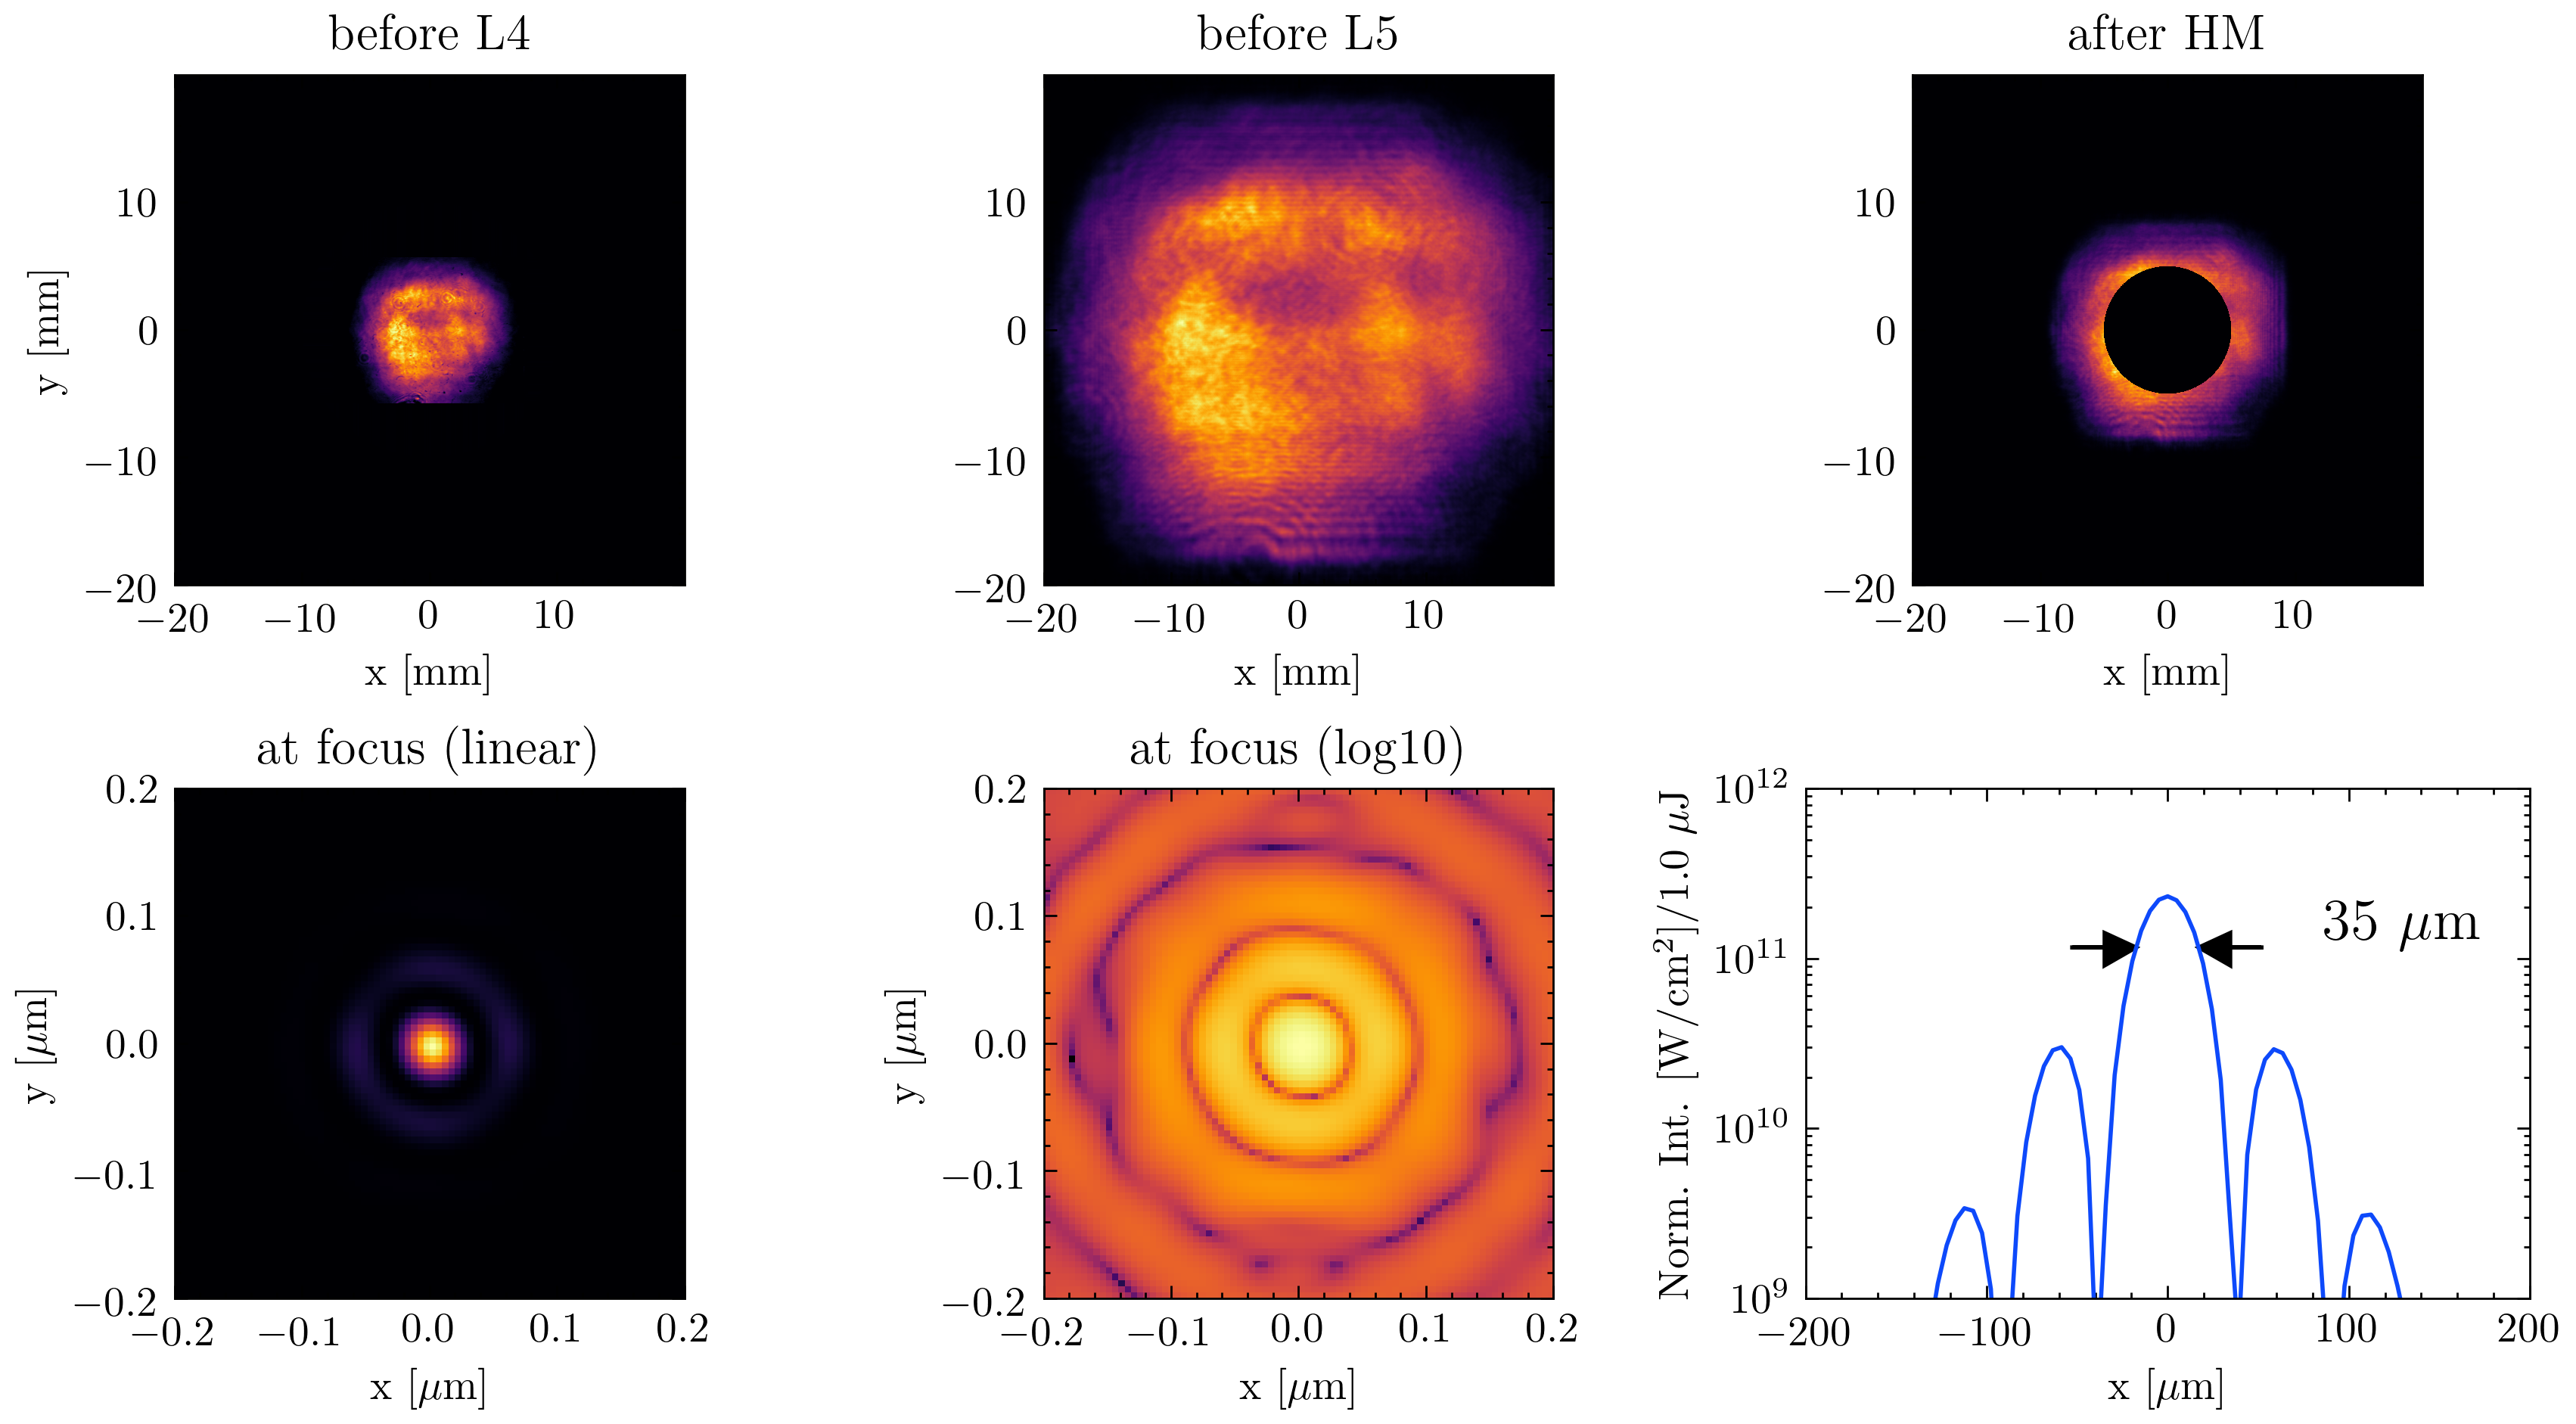
\includegraphics[width=0.75\textwidth]{figures/chap3/pump_on_focus_calculation_8192_inferno.png}
	\caption{Numerical propagation of the IR ($\lambda$=1500 nm) beam through the pump arm. Beam path layout follows \cref{fig:beamline_schematic}. Each panel shows the intensity of the beam as the beam propagates towards the focus. The first panel shows the measured intensity (Electrophysics PV320 thermal camera), all other panels are calculations. The arrows on the lineout indicate FWHM. All calculations are for vacuum (n=1). See text for details.}
	\label{fig:pump_on_focus_calculation}
	% plot made with \Python Scripts\LightPipes\pump_intensity.py using N=2**13 gridside
\end{figure}

The profile of the TOPAS output at $\lambda$=1500 nm was measured immediately before diverging lens L4 using an Electrophysics PV320 thermal camera. The beam was propagated numerically using the Python package \textit{Lightpipes for Python} \cite{vdovinLightPipesPython} through the remainder of the pump arm towards the focus using a grid size of $2^{13}\times2^{13}$. The result of this calculation is shown in \cref{fig:pump_on_focus_calculation}. Optical element parameters are as follows: L5 is a $f = +500 \text{ mm}$ Thorlabs LA1380-C, located 68.5 cm after L4 ($f = -300 \text{ mm}$, Thorlabs LF1015-C). The hole mirror HM is located 53 cm after L5 and has an inner radius of 5 mm. Clear apertures of 22.86 mm (L4), 45.72 mm (L5) and 50.8 mm (HM) were assumed. A 65 fs Gaussian temporal profile containing 1 $\mu$J of energy was assumed.

Reflection losses from the 2 Ag mirrors, 2 AR-coated lenses and uncoated $\text{CaF}_2$ vacuum window are responsible for a 26.2\% reduction in transmitted power. Additionally, the geometry of the hole mirror causes only 56\% of incident power to be incident on a reflective surface (the rest is lost to the central aperture). In total, the pump arm transmits 41.3\% of the power from before L4 to the focus.

The IR intensity makes an Airy-like diffraction pattern at the focal plane. There is an intense bright spot surrounded by a series of rings, with the intensity of each ring as the distance from the center increases. The rings exhibit a periodic modulation in intensity with respect to angle $\phi$. This four-fold symmetry is due to the square-like spatial profile of the TOPAS output, whereas the clipping from the hole mirror's aperture is responsible for the central peak and ring structure. The central lobe has a peak intensity of $\sim 2.3 \times 10^{11} \text{ W/cm}^2$ per 1 $\mu$J input pulse energy and a FWHM of 35 $\mu$m. The first ring has a radius of 59 $\mu$m and a peak intensity $\sim 2.9 \times 10^{10} \text{ W/cm}^2$ per input $\mu$J pulse energy. Thus the central lobe's peak intensity is about an order of magnitude larger than the ring's intensity. However, the central spot only contains about 49\% of the total power, as the rings cover a much larger area.

Note that the above calculations assume perfect alignment into the hole mirror (i.e., the IR beam is centered on the central aperture of the hole mirror). If the IR beam is misaligned to the hole mirror, then the transmission to the focus will increase as the most intense part of the beam is no longer clipped by the central aperture. Therefore, a drift in the laser's pointing during an experiment can effect the sample's interaction intensity.

\subsection{Estimation of Excited Carrier Density}
\label{sec:Excited_Carrier_Density}

\begin{figure}
	\centering
	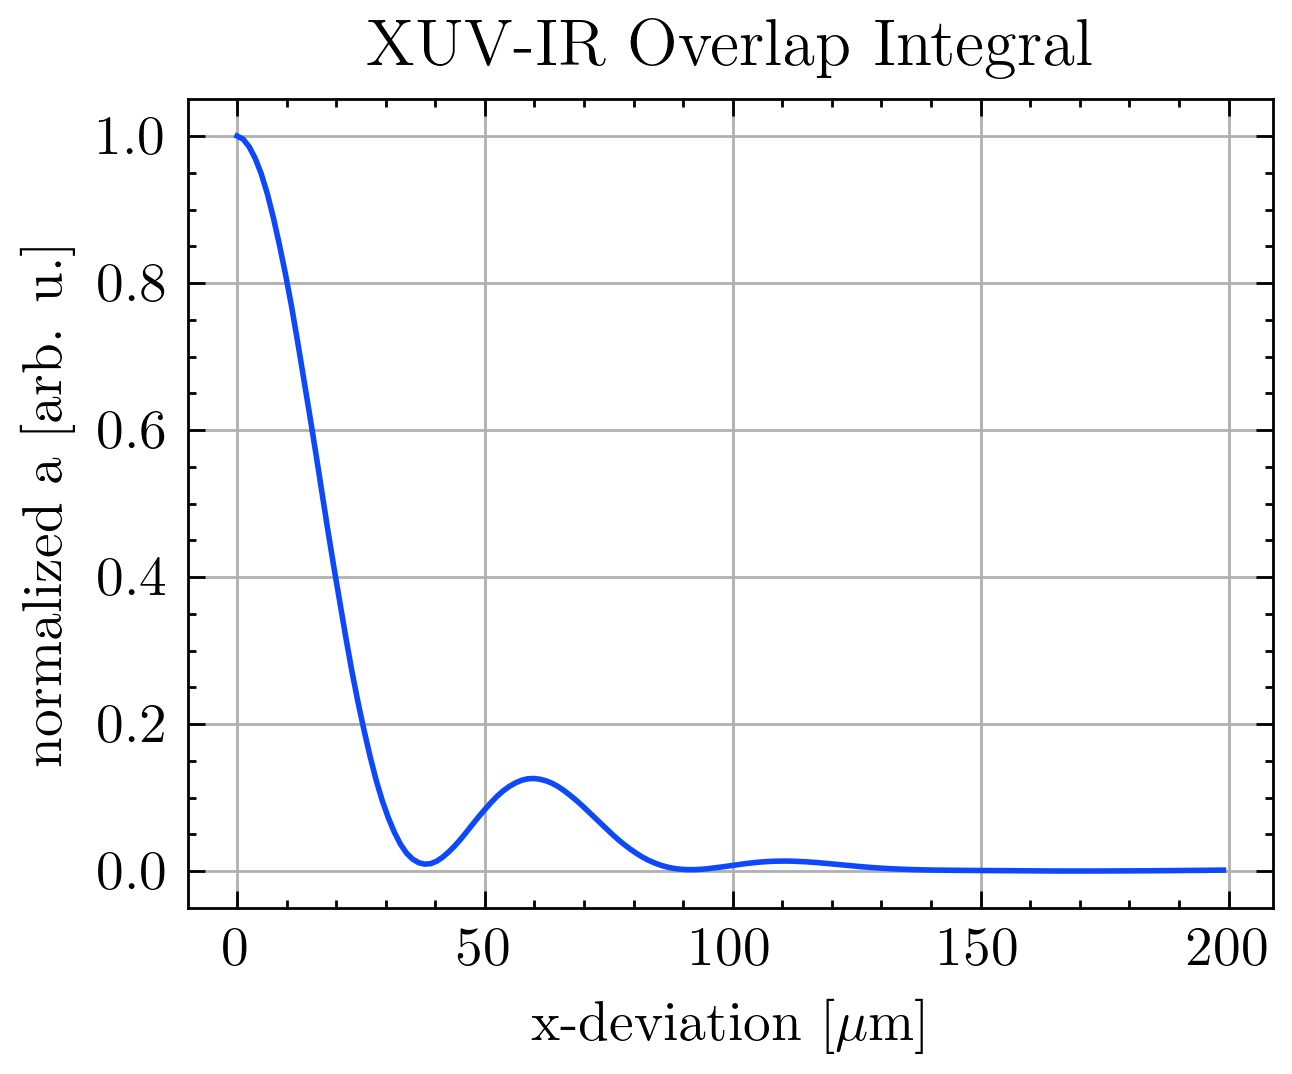
\includegraphics[width=0.5\textwidth]{figures/chap3/XUV-IR_overlap_integral.png}
	\caption{XUV-IR overlap function, as defined in \cref{eqn:XUV-IR_integral}, calculated using the numerical simulation results of \cref{fig:pump_on_focus_calculation} and a Gaussian XUV beam with a 6 $\mu$m waist. The result has been normalized to perfect overlap. \textbf{NOTE: change the y-axis label to something like $a / a_{max}$, and the x-axis label to $x_0$.}}
	\label{fig:XUV-IR_integral}
	% plot made with \Python Scripts\LightPipes\pump_intensity.py using N=2**13 gridside
\end{figure}

We are concerned with two quantities: the peak excitation fraction in the sample and the average excitation fraction at the location of the XUV focus. The former quantity is relevant when considering sample damage, whereas the latter will be proportional to the measured signal. If the XUV and IR spots are perfectly overlapped at the sample plane, then these two quantities are equal. We first calculate the peak excitation fraction, then we consider how a misaligned beam will effect the measured signal.

The electric field inside the sample $E_{\text{int}}$ is related to the external electric field by the following equation \cite{schultzeAttosecondBandgapDynamics2014}:
\begin{equation}
E_{\text{int}} = \frac{2}{1+\sqrt{\epsilon}} E_{\text{ext}}
\label{eqn:internal_external_Efield}
\end{equation}
where $E_{\text{int}}$ is the electric field inside the sample, $E_{\text{ext}}$ is the electric field outside the sample, $\epsilon$ is the dielectric constant and its square root is the refractive index $n_{\text{IR}}$. The internal intensity $I_{\text{int}}$ is the square of the internal electric field. For germanium at $\lambda$ = 1430 nm, $n_{\text{IR}}$ = 4.2481, and we have the following relations:
\begin{equation}
\begin{aligned}
E_{\text{int}} &= 0.381 \times E_{\text{ext}} \\
I_{\text{int}} &= 0.145 \times I_{\text{ext}}
\end{aligned}
\end{equation}

Given our laser paremeters, we can estimate the highest carrier density within the sample. First, we estimate the absorbed laser fluence, $F_{\text{abs}}$ \cite{harbCarrierRelaxationLattice2006}:
\begin{equation}
F_{\text{abs}} = F_{\text{inc}} \left(1-R\right) \left( 1-\exp(-\alpha L) \right) \left(1+R \exp(-\alpha L)\right),
\label{eqn:absorbed_fluence}
\end{equation}
where $F_{\text{inc}}$ is the incident fluence, $R$ is the reflectivity equal to the square of the Fresnel coefficient, $\alpha$ is the absorption coefficient and $L$ is the sample thickness. The bracketed terms in \cref{eqn:absorbed_fluence} are the fraction of fluence transmitted by the first surface, the fraction absorbed by a single pass through the sample, and the additional absorption due to a back reflection off the rear face of the sample. Note that the back-propagating beam will arrive (on average) at a delay of $n_{\text{IR}} L/(2c) \approx 0.7 \text{ fs}$ later than the forward-propagating beam. This time scale is nearly two order of magnitude less than the pulse duration, so we should expect any electron dynamics initiated by the back reflection to contribute to the measured signal.

If each absorbed photon corresponds to an excited electron, then the excited carrier density $\Delta N$ is given by the following expression \cite{cushingDifferentiatingPhotoexcitedCarrier2019}:
\begin{equation}
\Delta N = \frac{F_{\text{abs}}}{\hbar \omega} \frac{1}{L},
\label{eqn:excitation_fraction}
\end{equation}
where $\hbar \omega$ is the IR photon energy. In \cref{eqn:excitation_fraction}, the quantity $F_{\text{abs}} / (\hbar \omega)$ represents the number of absorbed photons per unit area; dividing this quantity by the sample thickness gives the number of absorbed photons per unit volume. This assumes that the skin depth of the material is greater than membrane thickness.

Finally, we convert the excited carrier density to a fractional excitation. Germanium has $N_{\text{u.c.}}=2$ valence electrons per unit cell, and each unit cell has a volume $V_{\text{u.c.}}=4.527 \times 10^{-23} \text{ cm}^{3}$. Therefore the fractional carrier excitation is
\begin{equation}
f = \Delta N \frac{V_{\text{u.c.}}}{N_{\text{u.c.}}}
\end{equation}

We can use literature values for 100 nm of germanium pumped at $\lambda$ = 1430 nm light. From the literature \cite{nunleyOpticalConstantsGermanium2016}, $R = 0.38315$, $\alpha = 5803.4 \text{ cm}^{-1}$, and so $F_{\text{abs}} = 0.0413 \times F_{\text{inc}}$. Therefore, only about 4.13\% of the incident fluence is absorbed by the sample.

According to the calculations in \cref{fig:pump_on_focus_calculation}, for each 1 $\mu$J energy input pulse (measured at L4), 0.413 $\mu$J makes it to the focal plane. 49\% of that energy is within the main lobe, which contains 0.202 $\mu$J of energy. Approximating the central lobe as a Gaussian beam with a FWHM of 35 $\mu$m and a pulse energy of 0.202 $\mu$J, the peak fluence is calculated by dividing the total energy of the Gaussian by $\pi w^2/2$. The Gaussian beam waist $w$ is related to the FWHM via $w^2 = \text{FWHM}^2 / (2 \ln 2)$. Thus, for each 1 $\mu$J input energy, the peak fluence in the central lobe is 14.6 mJ/cm$^2$ and the absorbed peak fluence is 0.60 mJ/cm$^2$. This corresponds to an peak excited carrier density of $4.3 \times 10^{20} \text{ cm}^{-3}$ and an excitation fraction of 0.98\% (per 1 $\mu$J of input energy).

\subsection{The XUV-IR Overlap Integral}

The excitation fraction can be computed for each spatial coordinate on the sample using the above method and the predicted intensity distribution from the numerical beam propagation calculations. Because the electrons are being excited via a single-photon process, the excited carrier density will be proportional to the fluence, and thus proportional to the intensity shown in \cref{fig:pump_on_focus_calculation}. Because the intensity of the XUV is very weak, the absorption of the XUV by the sample is also linear. Thus, we should expect the ATAS signal to be proportional to the XUV-IR overlap integral:
\begin{equation}
a = \frac{ \int dV \text{ } I_{\text{IR}} I_{\text{XUV}} }{ \int dV \text{ } I_{\text{IR}} \int dV \text{ } I_{\text{XUV}} }
\label{eqn:XUV-IR_integral_volume}
\end{equation}
Here, the integration volume is over the entire sample. If we assume that the intensity distribution does not appreciably change over the thickness of the sample, we can simplify the above equation. This is a reasonable assumption because the sample ($L = 100 \text{ nm}$) is much thinner the Rayleigh range ($z_R \sim 1 \text{ mm}$), and the absorption is low ($\sim 4\%$). So we assume the sample is a $\delta$-function in thickness and only evaluate the intensities at the focal plane. With this assumption, the overlap integral becomes:
\begin{equation}
a = L \frac{ \int dA \text{ } I_{\text{IR}} I_{\text{XUV}} }{ \int dA \text{ } I_{\text{IR}} \int dA \text{ } I_{\text{XUV}} }
\label{eqn:XUV-IR_integral}
\end{equation}
Knife edge measurements have been performed on the XUV light, showing that it has a Gaussian spatial profile with a beam waist of 6 $\mu$m. We write down the spatial profile of the XUV light at the focus:
\begin{equation}
I^{XUV} = I_0^{XUV} \exp \left( - 2 ((x-x_0)^2 + (y-y_0)^2) /  w_{XUV}^2 \right)
\end{equation}
Here, $I_0^{XUV}$ is the peak intensity and $w_{XUV}$ is the beam waist (radius), defined as the point where the intensity falls to $e^{-2} = 13.5\%$ of its maximum. The lateral shift from the center of the IR focal spot in the horizontal and vertical directions is $x_0$ and $y_0$, respectively. With this formulation, and using the simulation results for the IR spot, the XUV-IR overlap integral is calculated as a function of XUV-IR misalignment $(x_0, y_0)$. This result is shown in \cref{fig:XUV-IR_integral}. Here, XUV beam is translated relative to the IR beam in the horizontal direction ($x_0$) and the overlap is computed from \cref{eqn:XUV-IR_integral}.

\cref{fig:XUV-IR_integral} shows the sensitivity of a condensed matter ATAS experiment to relative alignment.\footnote{Note that the relevant parameter in \cref{eqn:XUV-IR_integral} is the relative positions of the two focal spots. We have yet to calculate the sensitivity of spatial overlap to deviations in the input laser pointing.} A spatial overlap deviation of 10 $\mu$m will cause the XUV-IR overlap - and thus the measured signal - to drop by 20\%. Note that a 10 $\mu$m displacement of the IR at the sample corresponds to a 15 $\mu$rad tilting of the hole mirror (HM). There are two ways misalignment can affect experimental results. If the relative positions of the XUV and IR focal spots changes as an experiment is performed, then the recorded ATAS signal would be a function of both the laser-induced dynamics and the XUV-IR spatial misalignment. On the other hand, if the entire experiment is performed using a constant misalignment, we would be exciting the sample to some peak excitation fraction $f$, but our probe would be measuring a lower excitation fraction ($\approx f a / a_{max}$). Consequently, the measured ATAS signal would be lower than otherwise expected, and any attempts to boost the signal by increasing the interaction intensity could result in permanent laser-induced sample damage.

A condensed matter ATAS experiment has much tighter alignment tolerances than a gas phase experiment. This discrepancy is a simple consequence of sample geometry and density. In either experiment, the measured signal comes from the region of space where the sample density, XUV intensity and IR intensity overlap. The transmission of XUV through the sample is, to first order, $T= \exp(- n \mu_a d)$, where $n$ is the number density, $d$ is the sample thickness and $\mu_a$ is the photoabsorption cross section. As discussed above, for technical reasons the experiment should be designed with $T \approx 1/2$. Therefore, the product $n \mu_a d$ will be approximately constant for any transient absorption experiment.

The number density of a condensed phase sample is determined by the chemistry of the compound and is on the order of $4 \times 10^{22} \text{ atoms}/\text{cm}^3$. The experimentalist is free to engineer clever sample geometries, heterostructures and/or nanopatterns, but the high atomic density (and thus absorption coefficient) dictates a total sample thickness on the order of 100 nm. On the other hand, the spatial profile and density of a gas phase sample is determined by the gas nozzle design and its backing pressure, respectively. A typical nozzle used in our lab produces a gas plume with lateral dimensions on the order of 200 - 500 $\mu$m. This effectively creates a sample that is three orders of magnitude thicker than a condensed phase sample, which relaxes the alignment constraints significantly. This has important consequences for the alignment of the sample.

If the XUV and IR are perfectly collinear, then the beam overlap region is effectively infinite in the propagation direction. In this case, the XUV-IR overlap integral will be positive regardless of any displacement of the sample plane from the focal plane, and maximal when the sample is at the focal plane. However, if there is a small angle $\delta \theta$ between their $k$-vectors, then the beams will only spatially overlap within a finite region. In this case, the position of the sample plane relative to the beam crossing plane becomes a critical experimental parameter. For an infinitely thick sample (i.e., a chamber effusively filled with gas), it wouldn't matter where the beams crossed as long as they overlapped somewhere within the chamber. Then, the overlap integral would decrease as a function of $\delta \theta$, but it would never go to zero. For a thin sample, the bounds of \cref{eqn:XUV-IR_integral_volume} must enclose the beam overlap region, or else the integral will be zero. Thus, the signal strength of a condensed phase ATAS experiment is roughly 3 orders of magnitude more sensitive to the $z$-position of the sample relative to the focal plane than a gas phase ATAS experiment.

\section{Experimental Methods}

In this section the methods to find spatial and temporal overlap of the XUV and IR are discussed. Also detailed are the experimental methods for adjusting the pump intensity for a condensed matter sample.

\subsection{Finding XUV-IR spatial overlap}
\begin{figure}
	\centering
	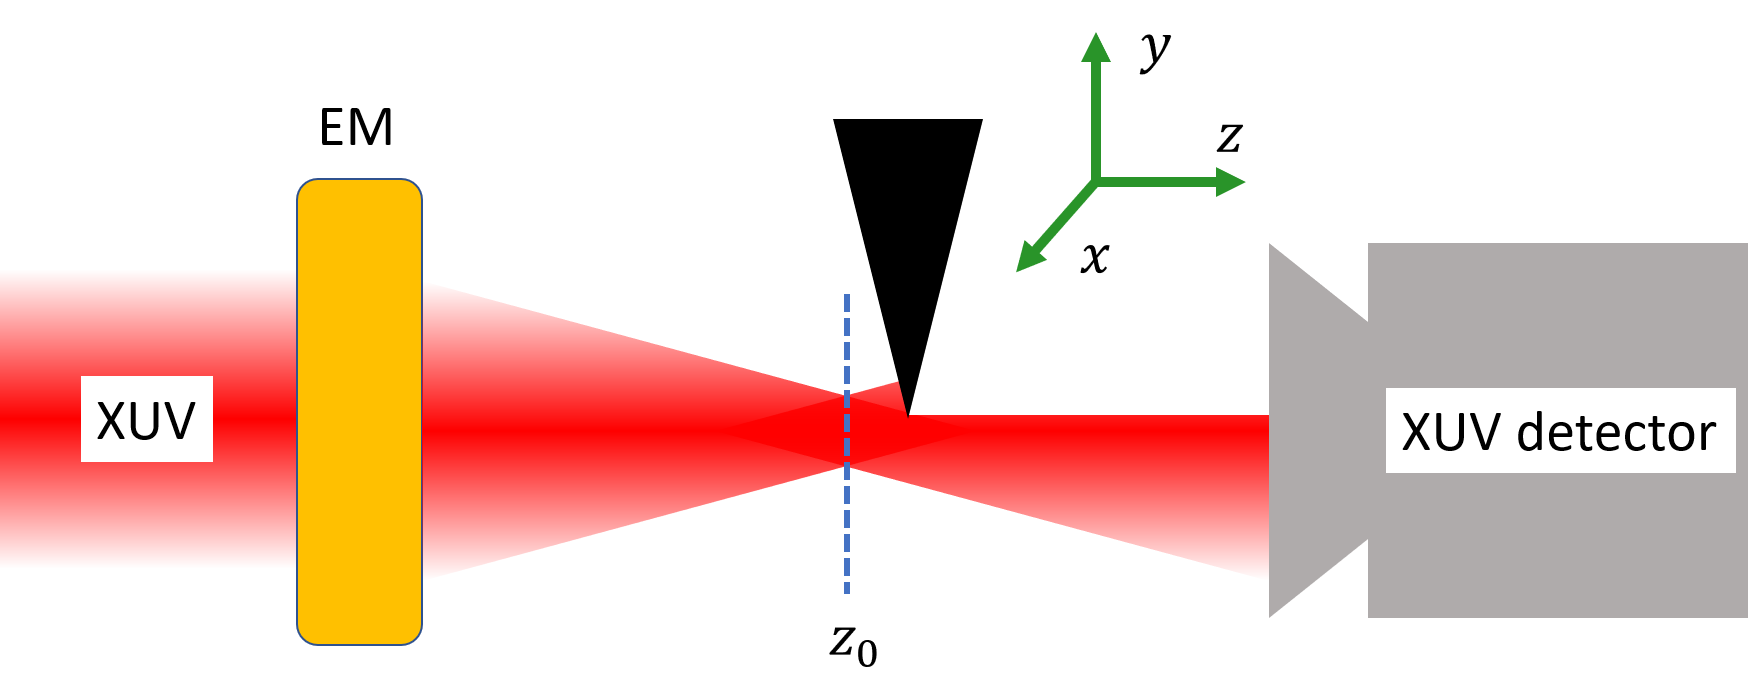
\includegraphics[width=0.75\textwidth]{figures/chap3/knife_edge_cartoon.png}
	\caption{Schematic of XUV knife edge measurement. EM: ellipsoidal mirror, $z_0$: XUV focal plane.}
	\label{fig:knife_edge_cartoon}
\end{figure}

\begin{figure}
	\centering
	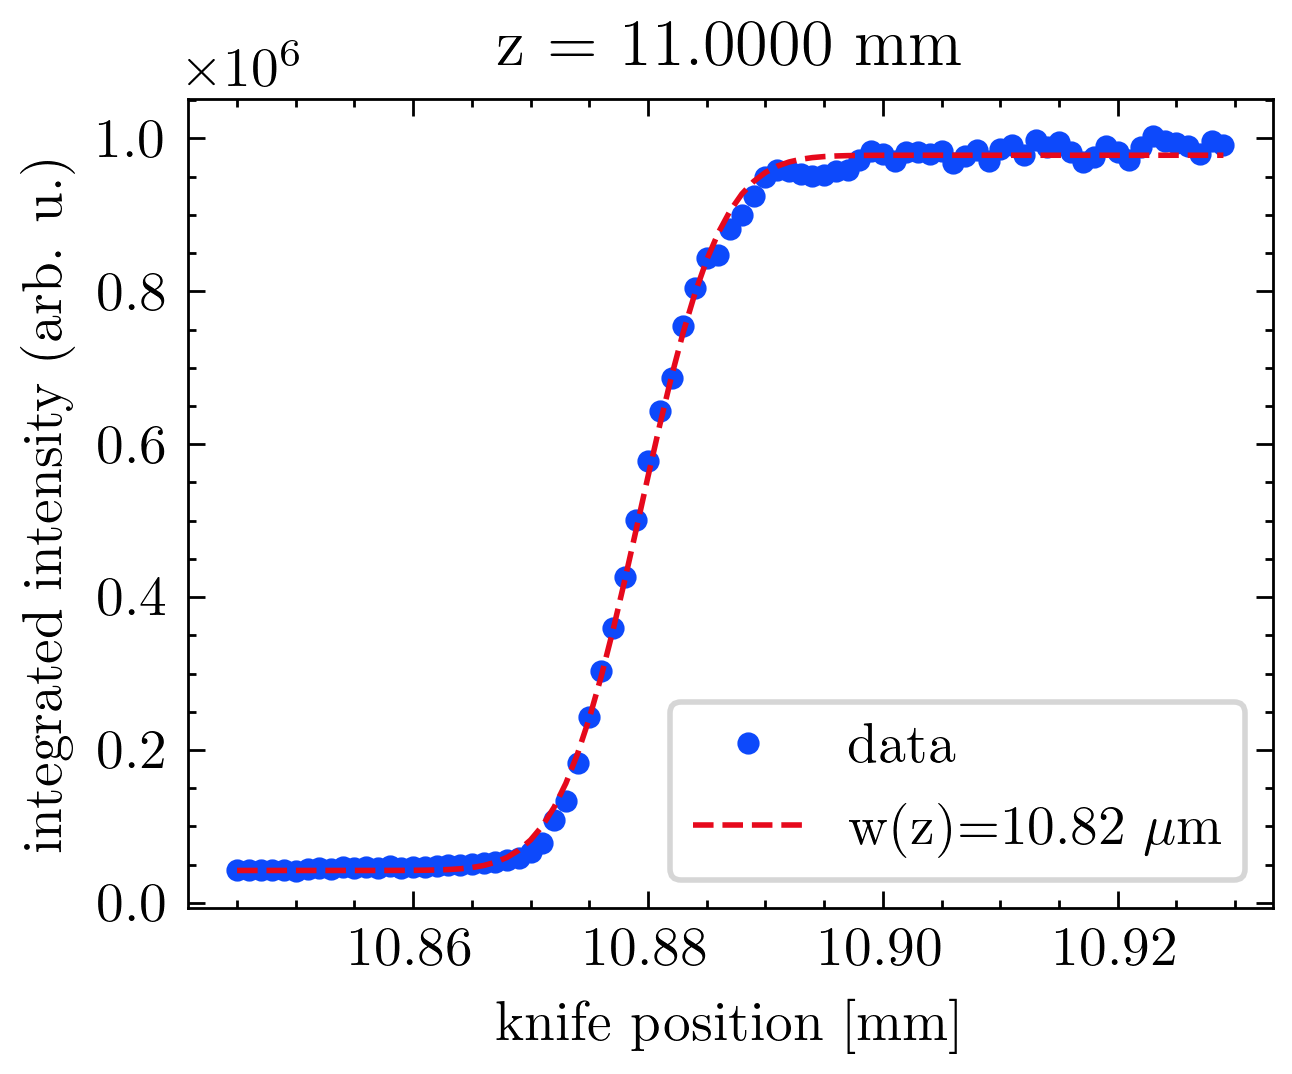
\includegraphics[width=0.75\textwidth]{figures/chap3/XUV_focus_knife_edge.png}
	\caption{A typical XUV knife edge measurement near the focal plane. The sample motor position is $k=11.0000$ mm. A fit to equation \cref{eqn:knife_edge} yields a beam waist of 10.82 $\mu$m at this position.}
	\label{fig:XUV_focus_knife_edge}
	% dataset: C:\testdata\2019_08_23\knife\11.0000
	% python file: \Python Scripts\Spectrometer\test\knife_edge.py
\end{figure}

\begin{figure}
	\centering
	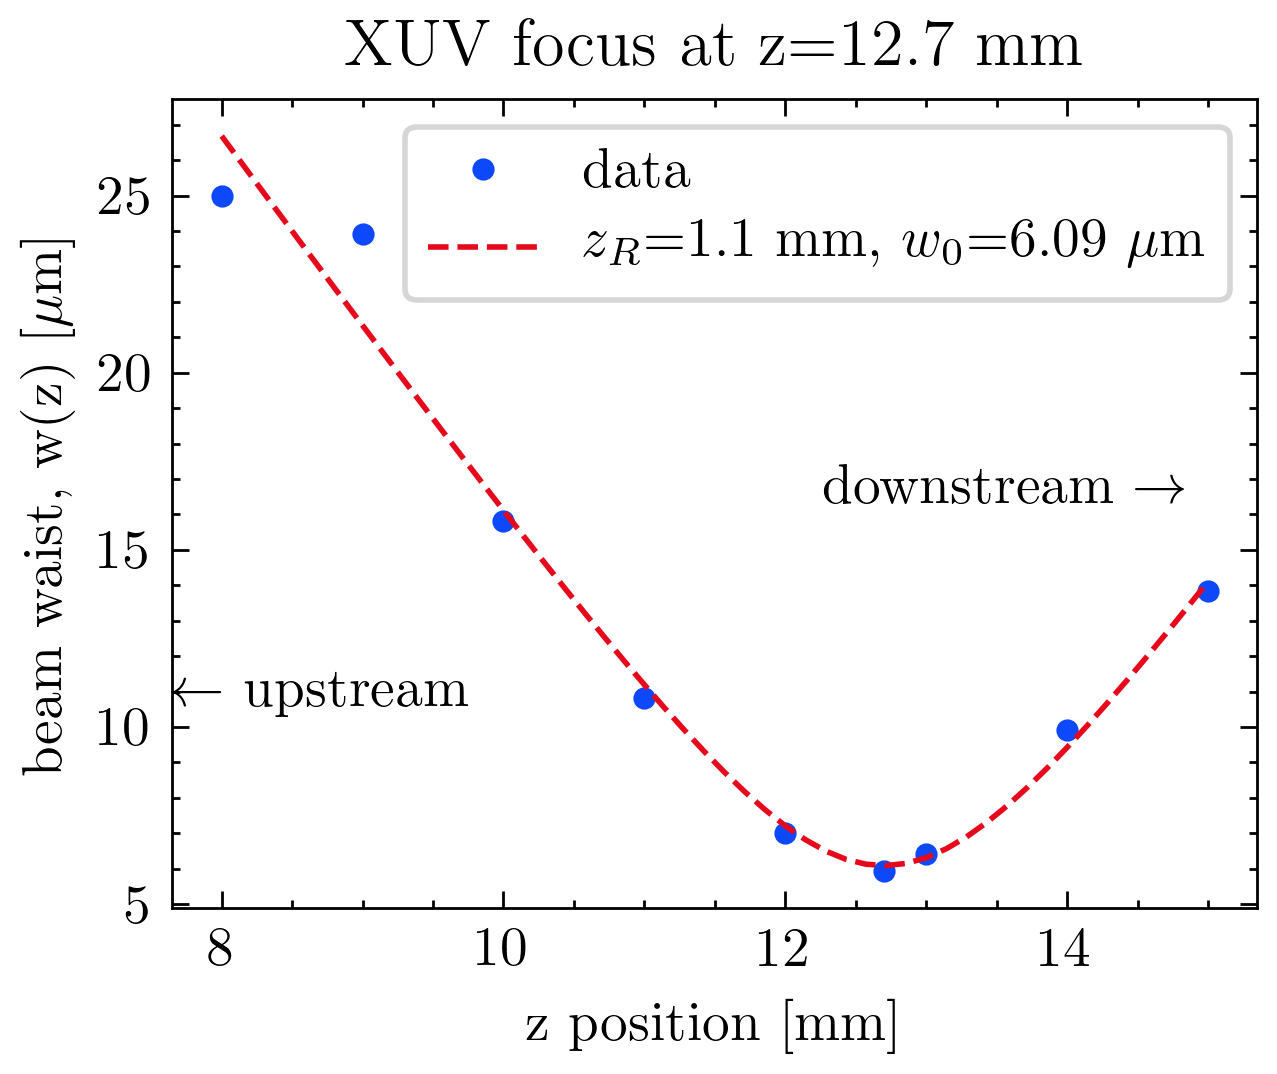
\includegraphics[width=0.75\textwidth]{figures/chap3/XUV_waist_vs_k.png}
	\caption{Evolution of XUV beam waist as a function of propagation direction, $z$. The Rayleigh range $z_R$ and beam waist $w_0$ are extracted from the fit to \cref{eqn:beam_waist_evolution}. \textbf{question: what is $M^2$ value of the XUV?}}
	\label{fig:XUV_waist_vs_k}
	% dataset: C:\testdata\2019_08_23\knife\11.0000
	% python file: \Python Scripts\Spectrometer\test\knife_edge.py
\end{figure}


XUV is ionizing radiation and cannot propagate in air. However, due to macroscopic phase matching conditions, the XUV propagates in the same direction as the IR light that created it. Therefore the initial alignment of the two arms of the interferometer is done by removing the metallic filter in the generation arm and overlapping the two IR foci in the target chamber. This alignment is done as follows.

First, we verify that the laser is pointing correctly into the interferometer using our fiducials.\footnote{Details of this process will be explained in the full dissertation.} We remove the sample holder from the target chamber and the metallic filter from the generation arm. This allows the generation arm's IR light to propagate downstream to the target chamber. We then place a pair of reflective and absorptive neutral density filters (OD = 7), a 1 $\mu$m low-pass filter (Thorlabs FELH1000) and a digital camera (ImagingSource DMK 27AUJ003) in the target chamber so the sensor is at the focus of the generation arm's IR light. These temporary optics are common to both arms, so they do not change the relative position of the foci. We close an iris before L3 to limit the intensity and note the position of the centroid of the focus on the camera's sensor. The generation shutter is closed and this process is repeated for the pump arm, with the power being controlled by the $\lambda /2$ waveplate-polarizer optics. The optical mount for the hole mirror has two vacuum compatible motors (Thorlabs Picomotors), which allow us to remotely change the two angles of this optic. By actuating these motors, we can control the lateral position of the pump arm's focus relative to the ellipsoidal mirror's focus. This process is iteratively repeated until the two foci are at the same location on the camera's sensor.

Due to phase matching, the optimal position of the high harmonic gas source is slightly downstream of the IR's focal position. As a result, the XUV will focus slightly upstream compared to the generation arm's IR that we used in the aforementioned alignment procedure. The exact distance between the gas cell and the IR focus depends on many factors, but it is on the few-millimeter scale. The ellipsoidal mirror has a 3:1 demagnification ratio, so for every 1 mm on-axis deviation in the generation chamber, we will have a $1/3^2 = 1/9$ mm on-axis deviation in the target chamber. A correction of this size is within the limit of our target chamber sample motors, but it must be done in vacuum using XUV light.

To this end, we must generate the XUV light that will be used for the upcoming experiment. With the chambers still vented, we verify temporal overlap (described below), and reinstall the sample holder is reinstalled. Finally, the chambers are pumped down and the generation conditions are adjusted to optimize the harmonic flux.

We characterize the XUV focus in the target chamber by performing knife edge measurements at different $k$-positions, as depicted in \cref{fig:knife_edge_cartoon}. We use the interior angled edge of the Si frame on a broken sample heterostructure as a knife edge (see \cref{fig:Sample_Geometry}). This frame makes an excellent knife edge as it has a very well-defined geometry and fits in the sample holder. Recalling Gaussian optics, the assumed profile of the XUV beam is:
\begin{equation}
I(x,y,z) = I_0 \left( \frac{w_0}{w(z)} \right)^2 \exp \left( - 2 ((x-x_0)^2 + (y-y_0)^2) /  w_(z)^2 \right),
\end{equation}
using the coordinate system defined in \cref{fig:knife_edge_cartoon}. The XUV focus is at position $(x_0,y_0,z_0)$. The beam waist $w(z)$ will evolve as:
\begin{equation}
w(z) = w_0 \sqrt{ 1 + \left( \frac{z-z_0}{z_R} \right)^2 },
\label{eqn:beam_waist_evolution}
\end{equation}
where $z_R$ is the Rayleigh range. If we use the knife edge to block the transmission as depicted in \cref{fig:knife_edge_cartoon}, then the transmitted power will be:
\begin{equation}
P(x, z) = P_0 + \frac{P_{max}}{2} \left( 1 - \erf \left( \frac{\sqrt{2}(x-x_0)}{w(z)} \right) \right),
\label{eqn:knife_edge}
\end{equation}
where $x$ is the insertion of the knife in the beam, $z$ represents the location of the knife plane in the propagation direction, and $\erf$ is the error function.

A typical knife edge measurement is shown \cref{fig:XUV_focus_knife_edge}. In this measurement, the knife edge is translated across the XUV spot in 1 $\mu$m steps until the XUV light is completely blocked. A 2D spectrum is saved at each knife edge position. Each image is background subtracted, normalized and summed (integrating over all divergences and wavelengths), which yields the XUV flux as a function of knife position. The resulting curve is fit to \cref{eqn:knife_edge} and the beam waist $w(z)$ is extracted for this $z$-position.

The knife edge measurement is repeated at different $z$-positions until enough data has been acquired to determine the focal plane. The evolution of the XUV beam waist is shown in \cref{fig:XUV_waist_vs_k}. In this figure, the beam waist has been fit to \cref{eqn:beam_waist_evolution} to determine the focal plane $z_0$, the Rayleigh range $z_R$ and the beam waist $w_0$. In both figures, a reasonably good fit is obtained, indicating that the XUV light has a Gaussian spatial profile near the focus.

It must be verified that the pump arm's IR light focuses to the same focal plane as the XUV. Therefore, the chambers are vented a second time, the sample holder removed, and the digital camera optics and filters installed. The k-position of pump arm's focus is moved up/downstream by moving L4, which is mounted on a translation stage.\footnote{The focusing optics in the pump arm are slightly chromatic, so L4 must be adjusted if the wavelength is changed.}

\subsection{Finding XUV-IR Temporal Overlap}

Temporal overlap can be found under vacuum or in air. In either case, spatial alignment must already be achieved. If the chambers are vented, temporal overlap can be checked using a camera at the focus to observe interference fringes. Note that the presence of air in the generation arm introduces an additional path length of $\approx (\text{3 m}) \times (n-1) \approx 820 \text{ } \mu \text{m}$. Therefore, the pump arm needs to be shortened by moving the retro reflector approximately $(\text{3 m}) \times (n-1)/(2n) \approx 410 \text{ } \mu \text{m}$ to recover overlap when the system is under vacuum.

Overlap can be found under vacuum by routing the IR beam outside of the chamber. A translatable silver mirror, controlled by a set of gears and a linear shift vacuum feedthrough, is used to direct the light through a viewport on the spectrometer chamber wall. The light is focused by a $f = +750$ mm lens (Thorlabs LA1727-C) onto a camera. Note that the spatial profile of the IR beam is not preserved during this routing, as the beam is heavily clipped by a vacuum aperture that separates the target chamber from the spectrometer. As a result, this method \textit{cannot} be used to confirm spatial alignment of the foci. However, enough light makes it through to view interference fringes at overlap. 

A BBO crystal, installed in one of the sample holder's sample slots in the target chamber, can also be used to find overlap. The intensity in each arm should be set so that SHG is produced only at temporal and spatial overlap.

\subsection{Experimental Determination of IR Pump Parameters}

\begin{figure}
	\centering
	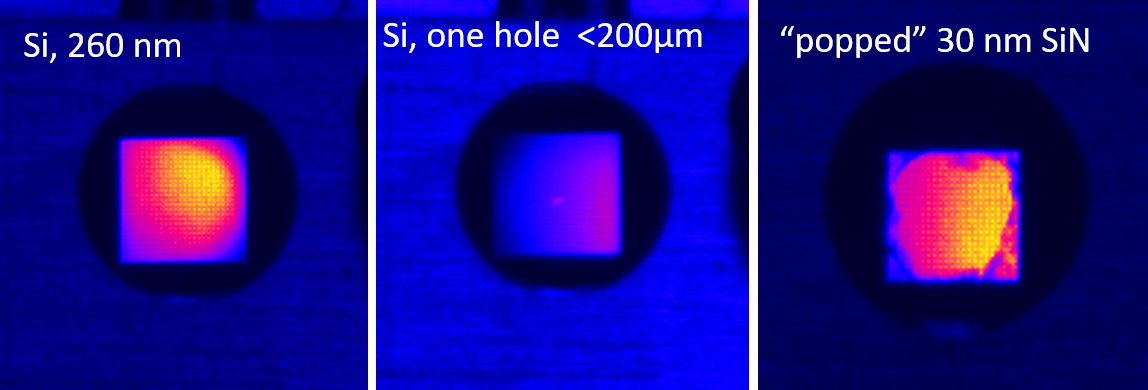
\includegraphics[width=0.75\textwidth]{figures/chap3/sample_damage.png}
	\caption{False color images showing laser drilled freestanding membranes. Left: pristine 260 nm thick Si membrane (Norcada). Middle: same sample, after a performing an IR power scan that exceeded the membrane's damage threshold. A $<$200 $\mu$m hole is visible as a cluster of bright pixels near the center of the membrane. Right: 30 nm SiN membrane after a similar power scan showing a ``popped'' membrane. The ragged edges near the clear aperture of the frame are all that remain of the membrane. For all images, the apparent brightness gradient across the samples is caused by inconsistent backlighting. Images were taken using the optical setup shown in the left panel of \cref{fig:sample_holder}.}
	\label{fig:sample_damage}
\end{figure}

\begin{figure}
	\centering
	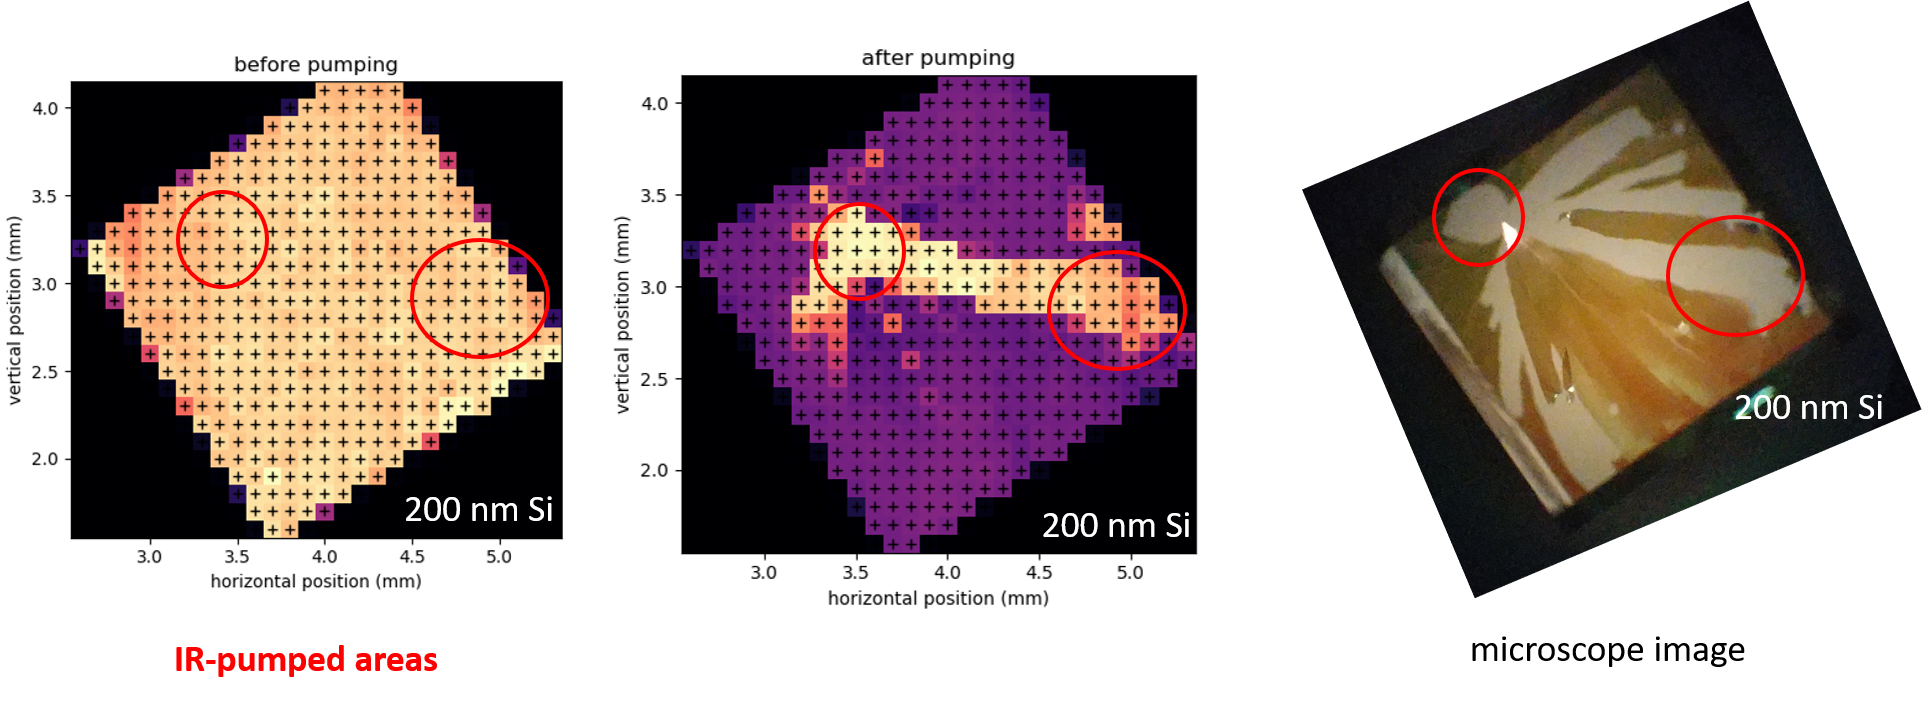
\includegraphics[width=0.75\textwidth]{figures/chap3/Si_damage.png}
	\caption{Laser damaged 200 nm silicon membrane samples. Left panel: XUV map of pristine Si before being exposed to IR laser. Higher transmission is indicated by brighter colors. Sample is rotated approximately 30 degrees relative to motor axes. Center panel: XUV map of damaged sample after being pumped with $\approx \text{ 65 }\mu$J of $\lambda = 1500 \text{ nm}$ at 1 kHz rep. rate in two locations. Damage occurred within the first camera exposure (2 seconds) and propagated to regions that were not exposed to the laser. Right panel: microscope image of damaged sample showing large sections of missing material. Red circles in all three pictures indicate the two locations that were exposed to IR laser light.}
	\label{fig:Si_damage}
\end{figure}

The arguments in \cref{sec:Excited_Carrier_Density} provide a starting point for the interaction intensity, but the optimum excitation intensity must be determined experimentally.

The IR intensity incident on the sample is controlled by a motorized achromatic $\lambda/2$ waveplate (Thorlabs AHWP10M-1600, $\lambda = 1100 - 2000$ nm) and a pair of ultra broadband wire grid polarizers (Thorlabs WB25M-UB, each with a 1000:1 extinction ratio for $\lambda = 0.6 - 4 \text{} \mu \text{m}$) in the pump arm (see \cref{fig:beamline_schematic}). A 1 $\mu$m longpass filter (Thorlabs FELH1000, $\text{OD}>5$) is positioned before the waveplate-polarizer assembly to filter out the OPA's visible parasitic wavelengths. During an experiment, the intensity is measured using an InGaAs photodiode (Thorlabs DET10D) mounted with a 2.0 absorptive neutral density filter and 1 $\mu$m longpass filter (Thorlabs FELH1000), which detects light scattered off a mirror in the pump arm and is monitored using an oscilliscope (LeCroy). Absolute measurements of the average IR power were taken with a power meter (Gentek) located before the diverging lens L4.

Permanent sample damage occurs when the sample is exposed to intensities above the damage threshold. The exact damage mechanism was not studied but we have observed two modes of failure, as shown in \cref{fig:sample_damage}. The most common failure mode results in the entire membrane shattering; occassionally only a pinhole will be drilled through the material. Sample damage is apparent in both the visible and the XUV, as shown in \cref{fig:Si_damage}. 

ATAS measurements were performed at 1 kHz, 500 Hz, 250 Hz and 125 Hz.

\subsubsection{1 kHz measurements}

\begin{figure}
	\centering
	\subfloat[$\tau \approx 0$ fs, PE = $1.03 \text{ } \mu \text{J}$.]{
		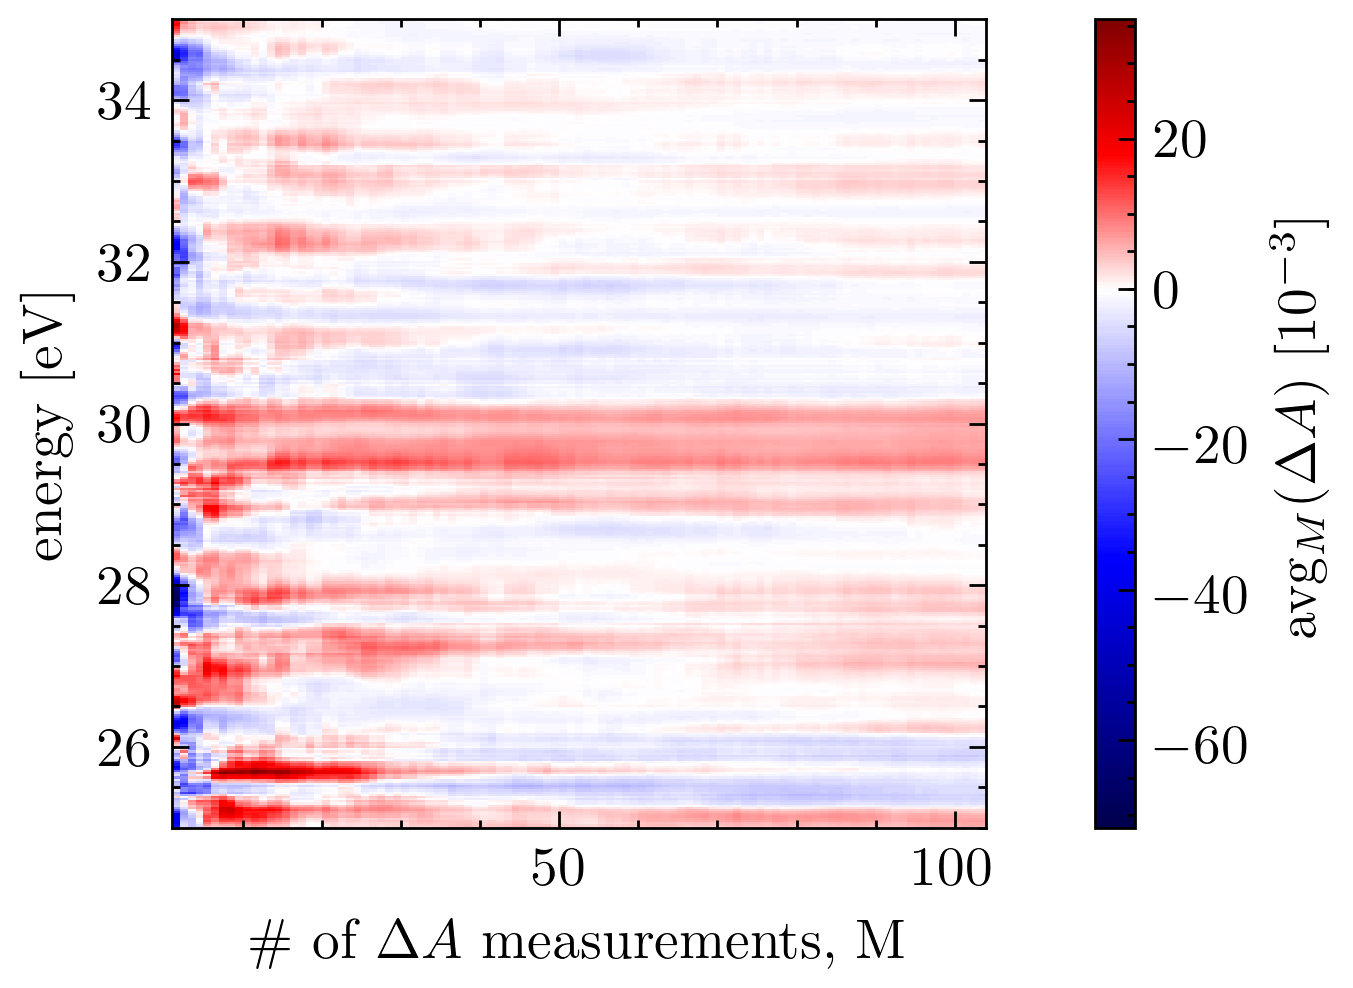
\includegraphics[width=0.4\textwidth]{figures/chap3/StaticOD_1kHz_overlap_1p03uJ.png}
		\label{fig:1kHz_Ge_ATAS:overlap_1.03uJ}}
	\qquad
	\subfloat[$\tau \approx 0$ fs, PE = $1.43 \text{ } \mu \text{J}$.]{
		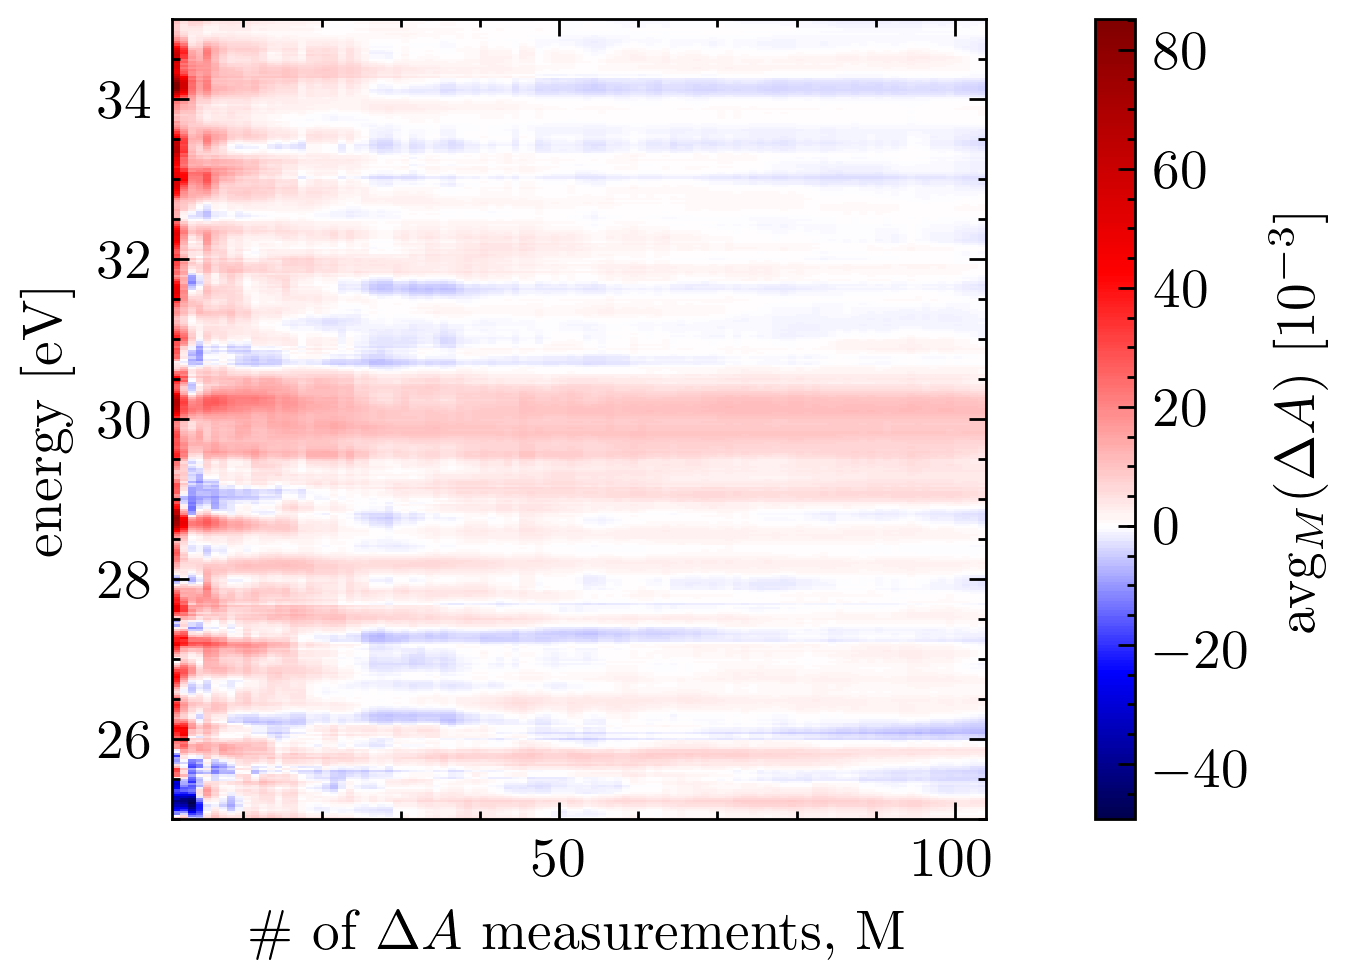
\includegraphics[width=0.4\textwidth]{figures/chap3/StaticOD_1kHz_overlap_1p43uJ.png}
		\label{fig:1kHz_Ge_ATAS:overlap_1.43uJ}}
	
	\subfloat[$\tau = - \infty$, PE = $1.03 \text{ } \mu \text{J}$.]{
		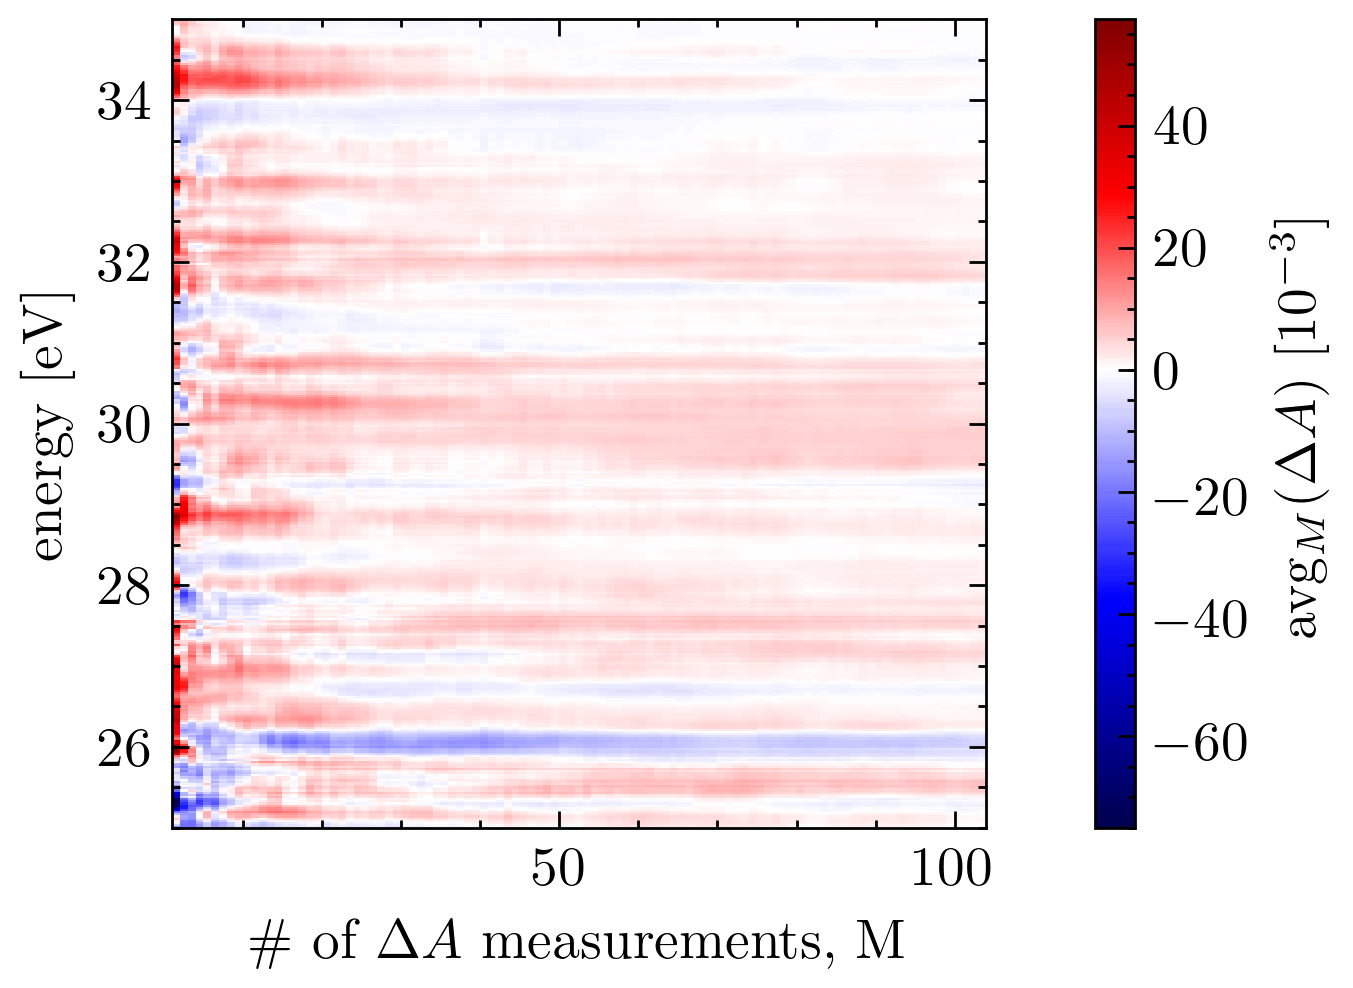
\includegraphics[width=0.4\textwidth]{figures/chap3/StaticOD_1kHz_NegInf_1p03uJ.png}
		\label{fig:1kHz_Ge_ATAS:NegInf_1.03uJ}}
	\qquad
	\subfloat[$\tau = - \infty$, PE = $1.43 \text{ } \mu \text{J}$.]{
		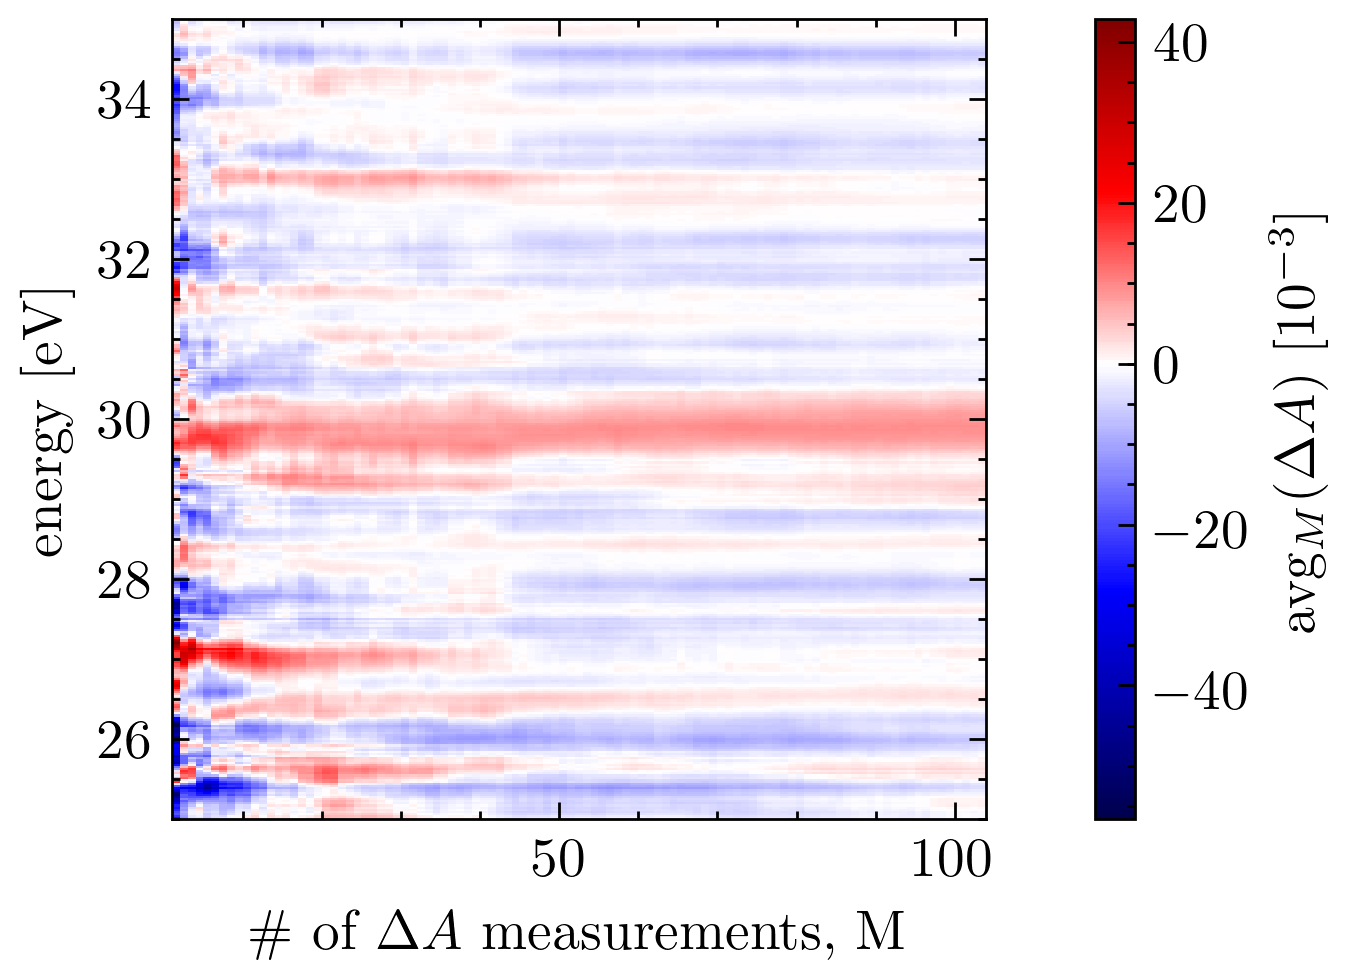
\includegraphics[width=0.4\textwidth]{figures/chap3/StaticOD_1kHz_NegInf_1p43uJ.png}
		\label{fig:1kHz_Ge_ATAS:NegInf_1.43uJ}}
	
	\subfloat[PE = $1.03 \text{ } \mu \text{J}$.]{
		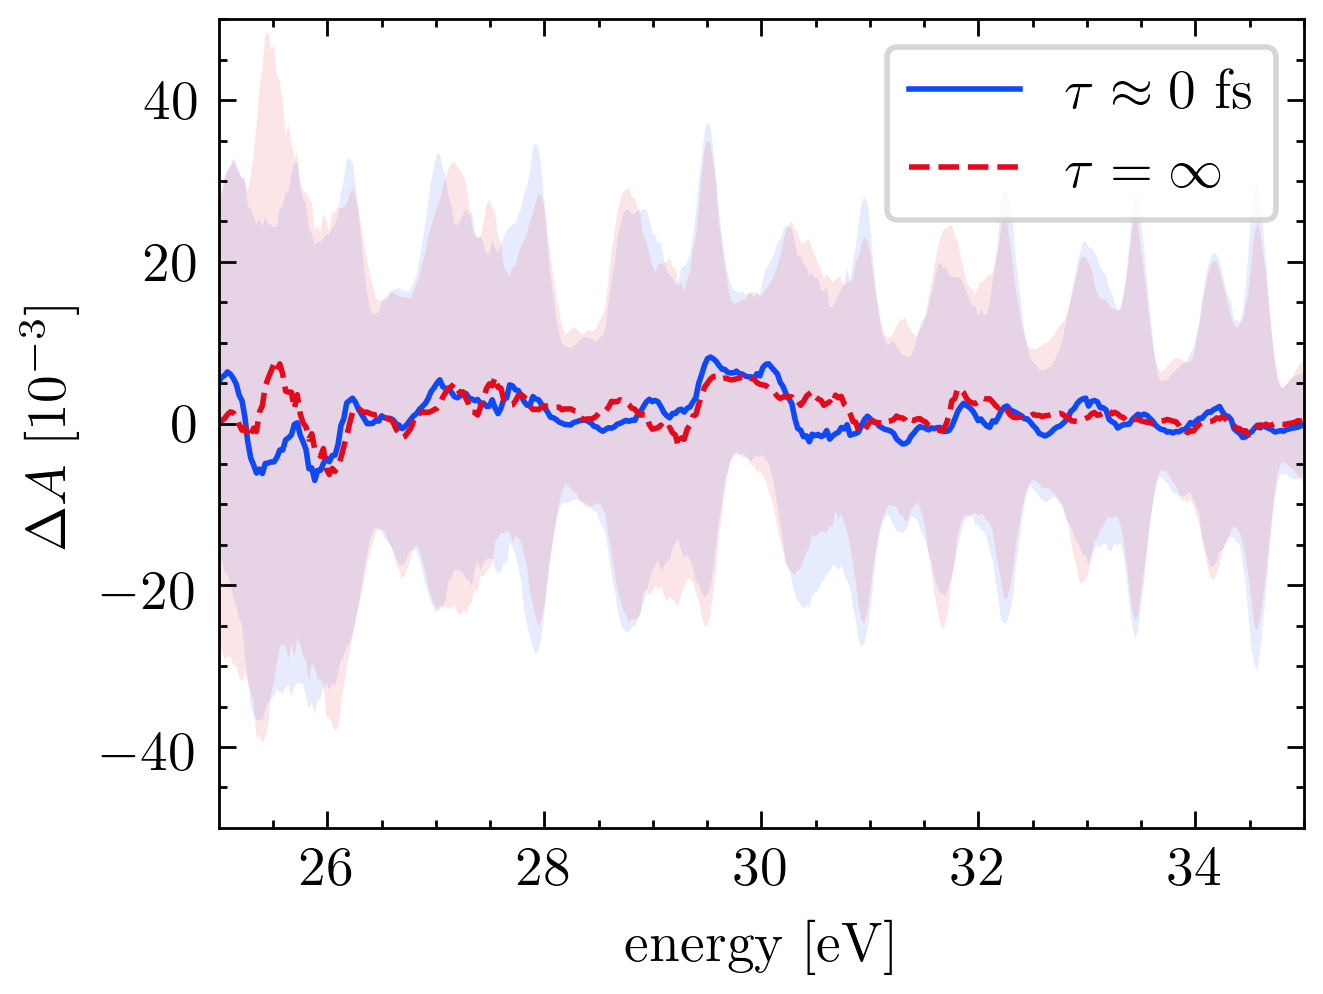
\includegraphics[width=0.4\textwidth]{figures/chap3/StaticOD_avg_1kHz_1p03uJ.png}
		\label{fig:1kHz_Ge_ATAS:avg_1.03uJ}}
	\qquad
	\subfloat[PE = $1.43 \text{ } \mu \text{J}$.]{
		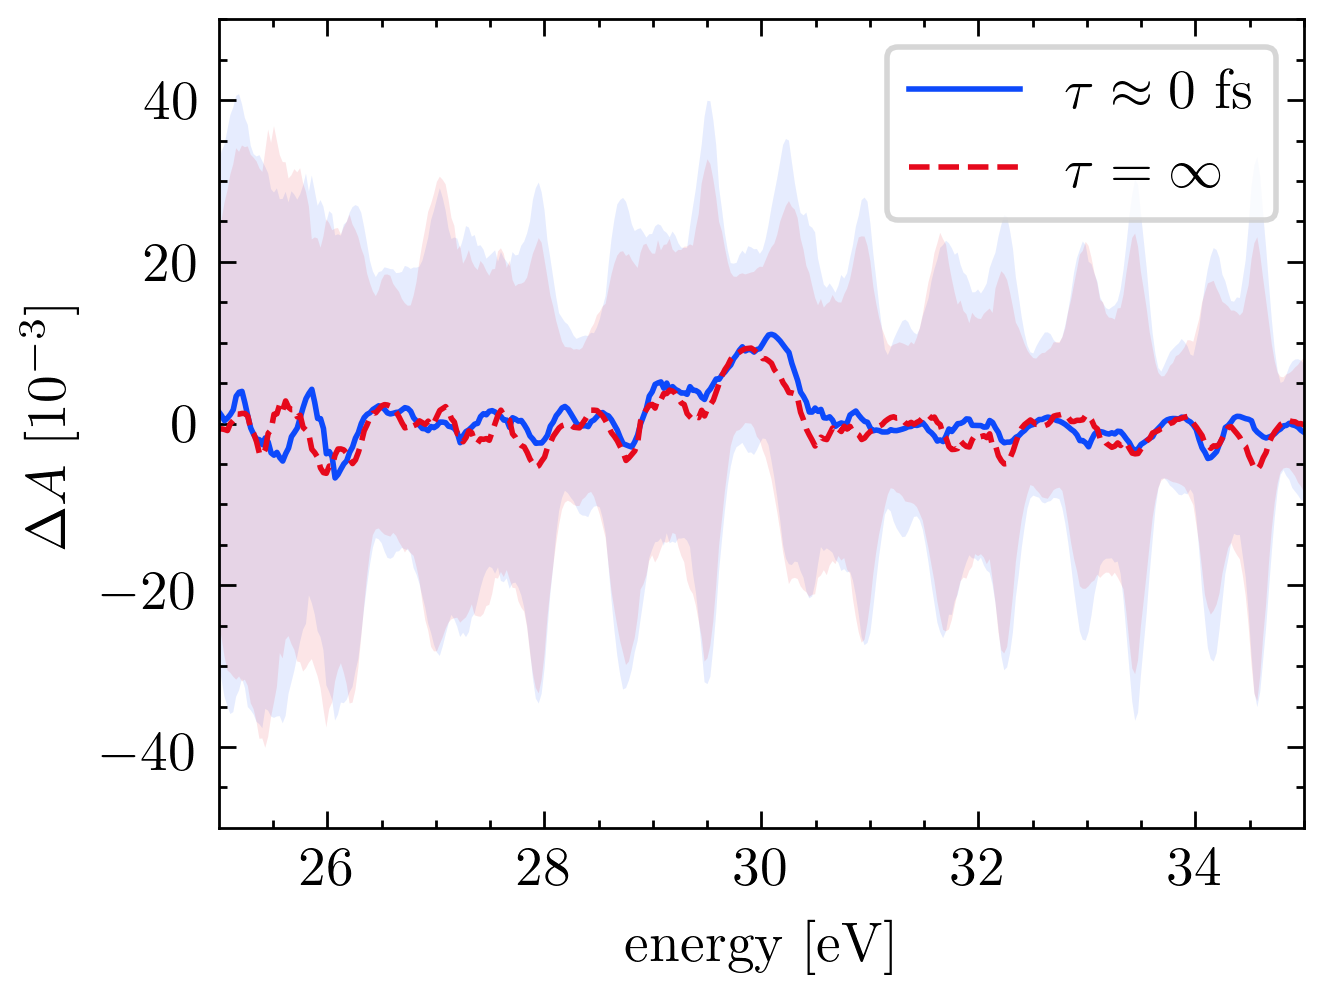
\includegraphics[width=0.4\textwidth]{figures/chap3/StaticOD_avg_1kHz_1p43uJ.png}
		\label{fig:1kHz_Ge_ATAS:avg_1.43uJ}}
	\caption{1 kHz fixed-delay ATAS measurements on 100 nm Ge using a $\lambda = 1450 \text{ nm}$ excitation pulse. See text for details.}
	\label{fig:1kHz_Ge_ATAS}
	% datasets: \testdata\2019_08_06\{Avg1,Avg3,Avg4,Avg5}
	% python script: \Python Scripts\Spectrometer\test\2019_08_06.py
\end{figure}

\begin{figure}
	\centering
	\subfloat[$\tau \approx 0$ fs, PE = $1.75 \text{ } \mu \text{J}$.]{
		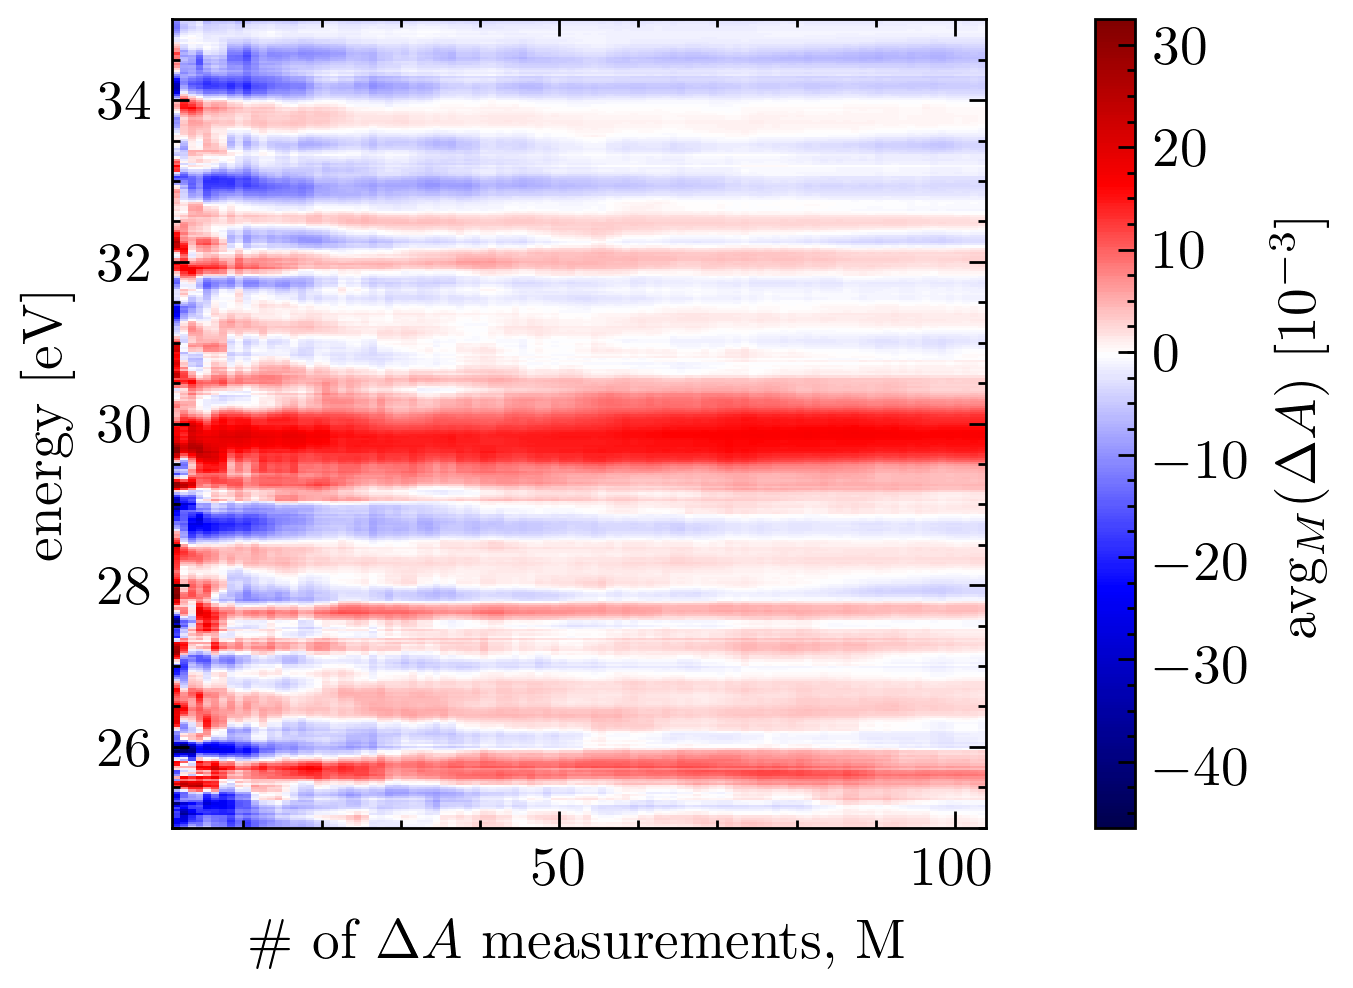
\includegraphics[width=0.4\textwidth]{figures/chap3/StaticOD_1kHz_overlap_1p75uJ.png}
		\label{fig:1kHz_Ge_ATAS:overlap_1.75uJ}}
	\qquad
	\subfloat[PE scaling at $\tau \approx 0$.]{
		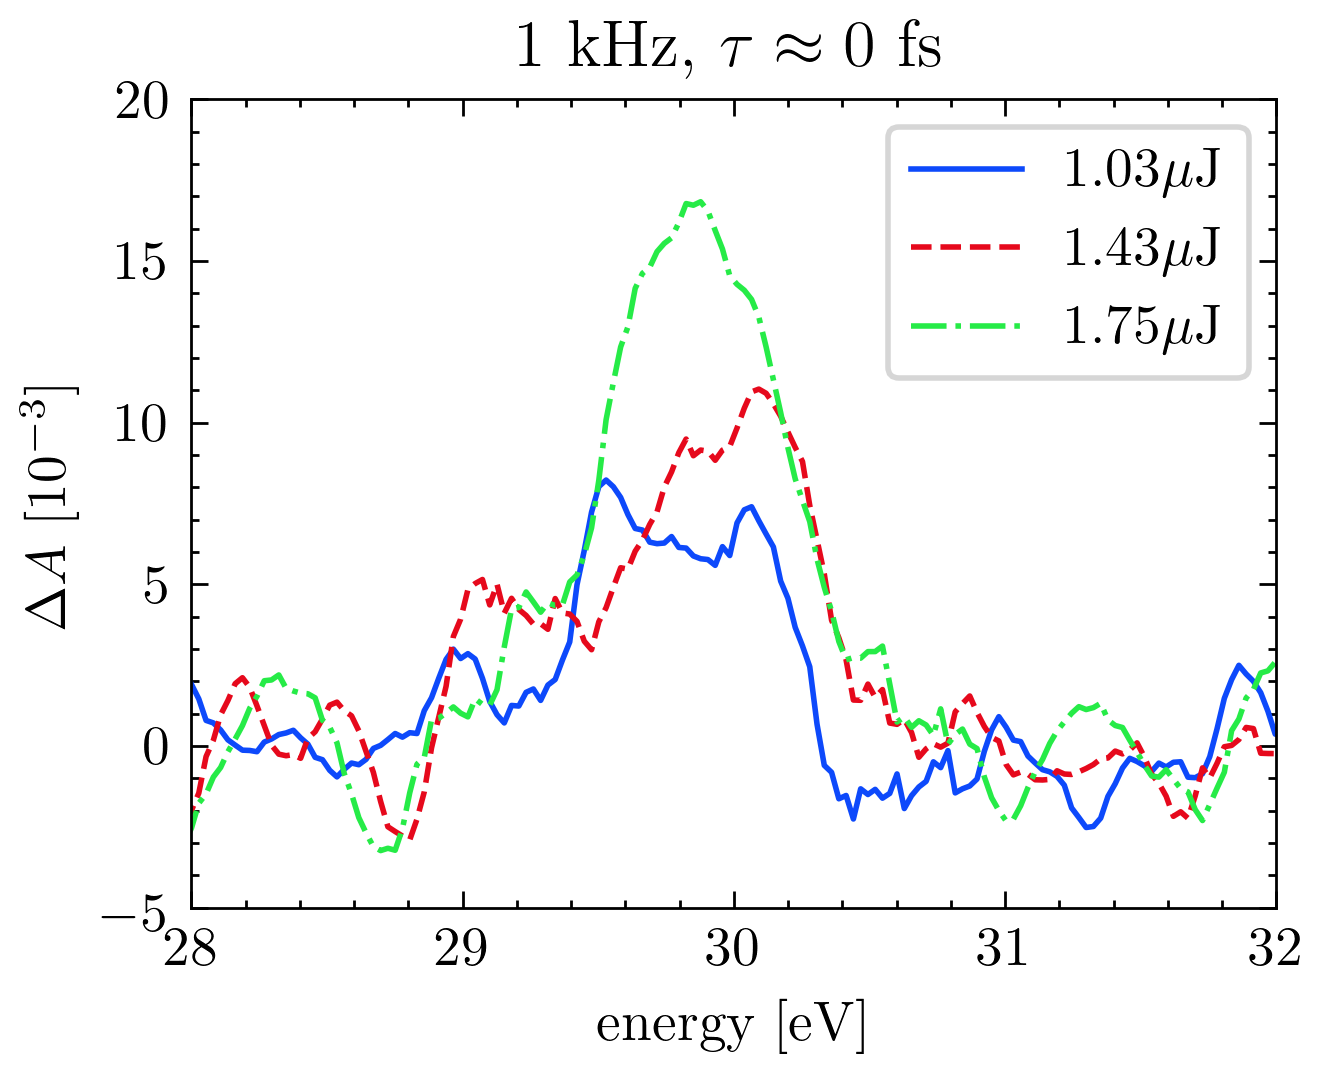
\includegraphics[width=0.4\textwidth]{figures/chap3/StaticOD_avg_1kHz_PE_scaling.png}
		\label{fig:1kHz_Ge_ATAS:PE_scaling}}

	\subfloat[PE = $1.43 \text{ } \mu \text{J}$.]{
		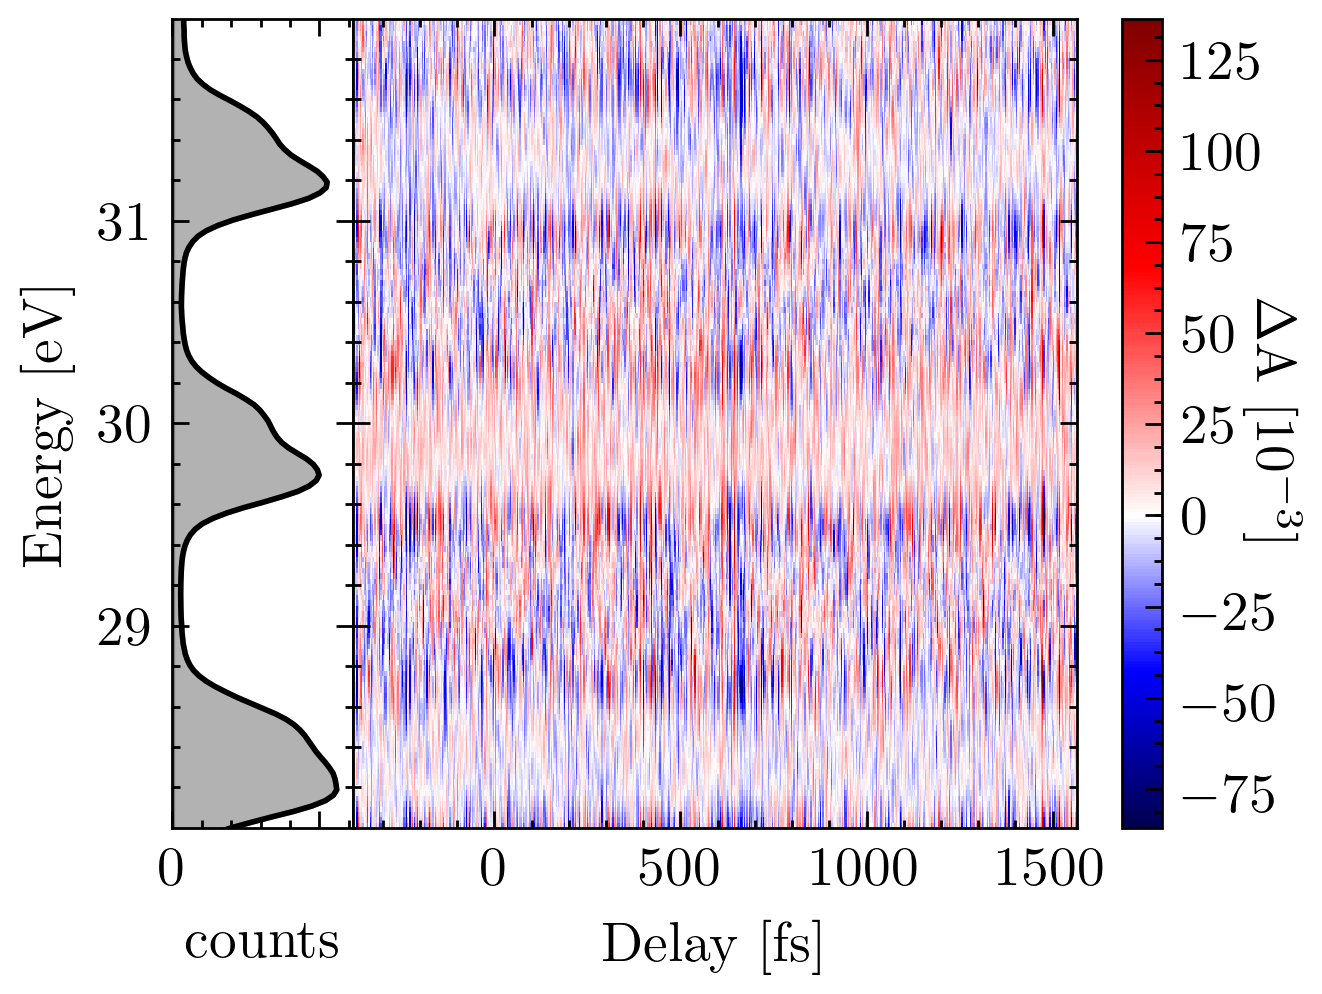
\includegraphics[width=0.4\textwidth]{figures/chap3/ODvsDelay_1kHz_1p43uJ.png}
		\label{fig:1kHz_Ge_ATAS:delay_1.43uJ}}
	\qquad
	\subfloat[PE = $1.75 \text{ } \mu \text{J}$.]{
		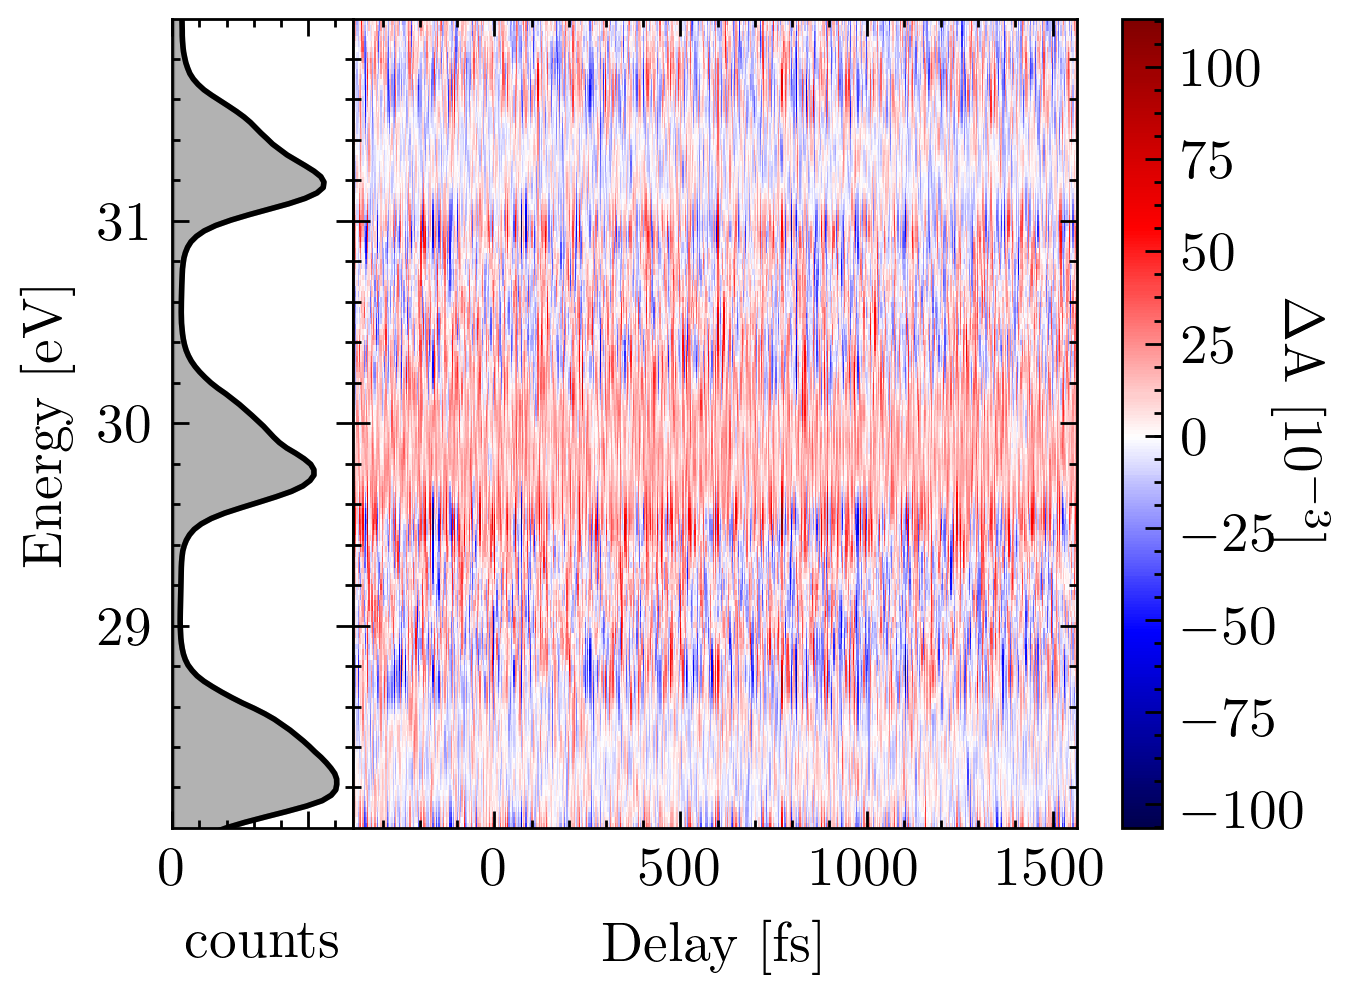
\includegraphics[width=0.4\textwidth]{figures/chap3/ODvsDelay_1kHz_1p75uJ.png}
		\label{fig:1kHz_Ge_ATAS:delay_1.75uJ}}
	
	\subfloat[PE = $1.43 \text{ } \mu \text{J}$ (rolling average).]{
		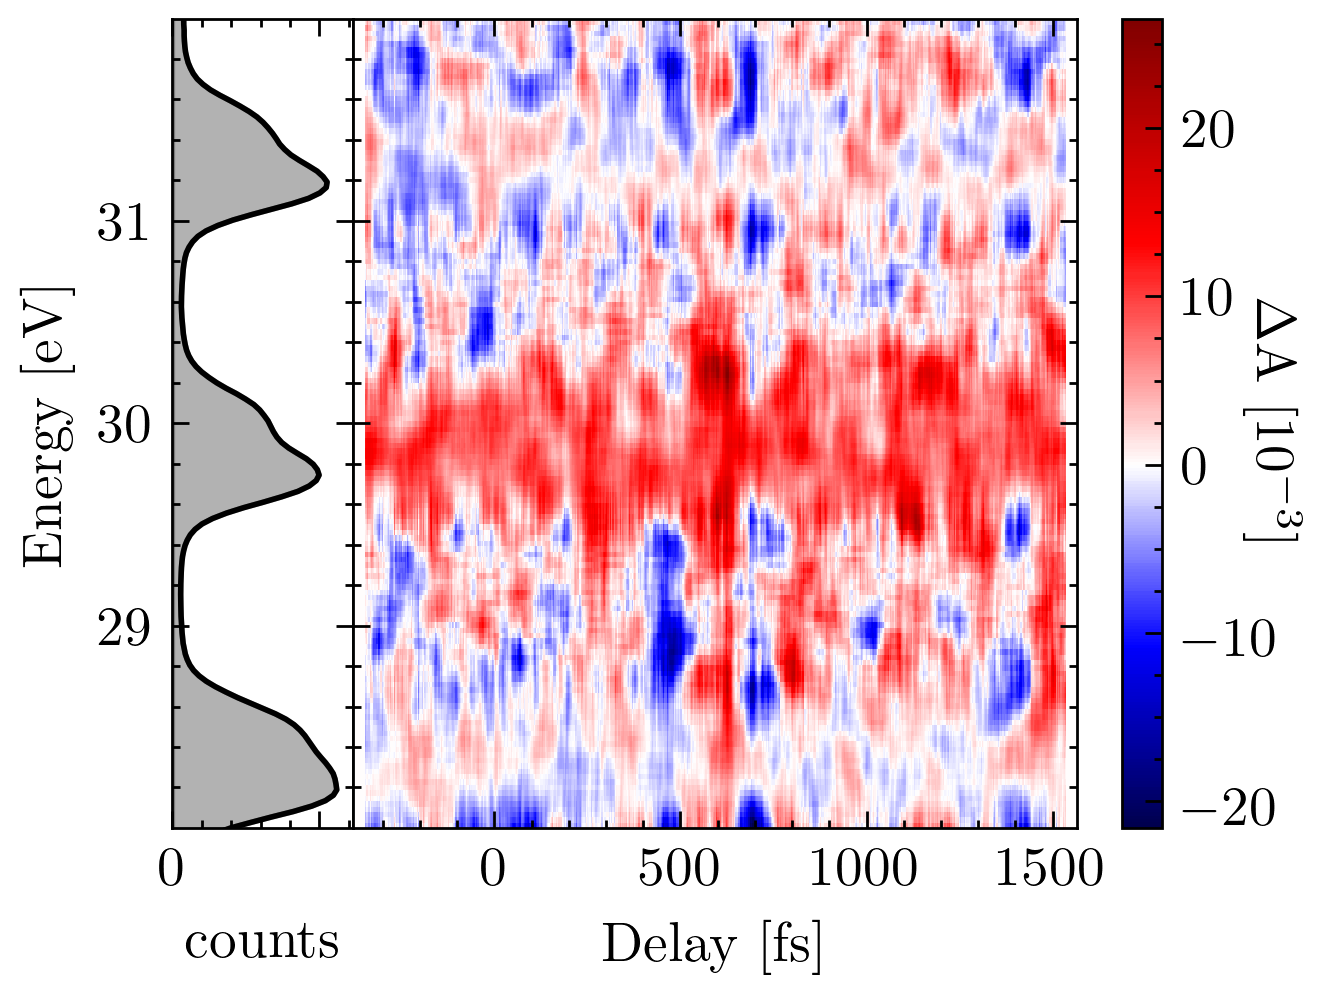
\includegraphics[width=0.4\textwidth]{figures/chap3/ODvsDelay_20roll_1kHz_1p43uJ.png}
		\label{fig:1kHz_Ge_ATAS:roll_delay_1.43uJ}}
	\qquad
	\subfloat[PE = $1.75 \text{ } \mu \text{J}$ (rolling average).]{
		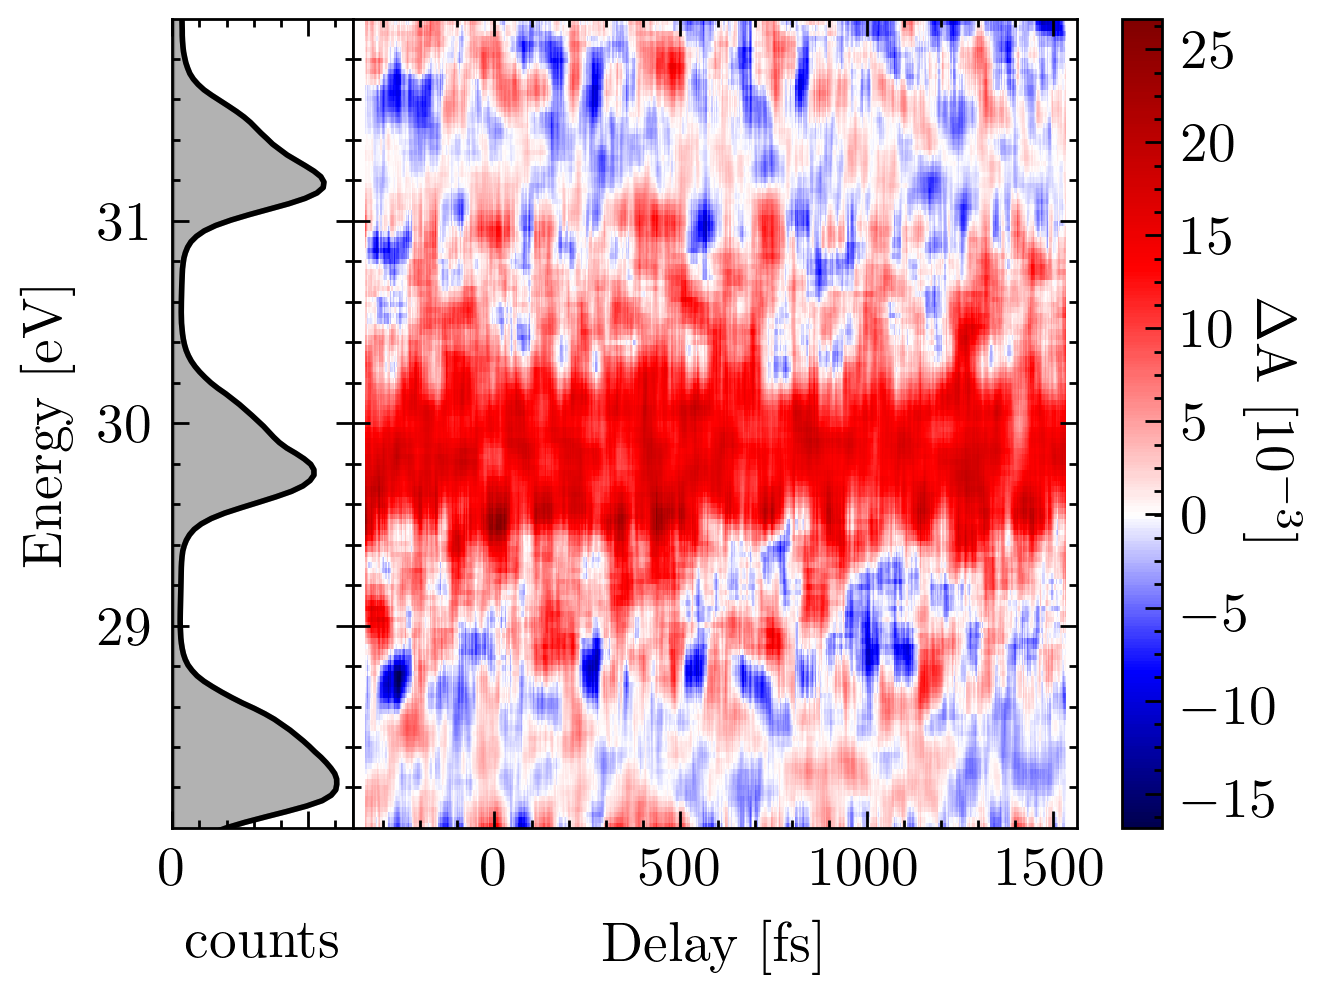
\includegraphics[width=0.4\textwidth]{figures/chap3/ODvsDelay_20roll_1kHz_1p75uJ.png}
		\label{fig:1kHz_Ge_ATAS:roll_delay_1.75uJ}}
	\caption{1 kHz ATAS measurements in Ge using a $\lambda = 1450 \text{ nm}$ excitation pulse.  \cref{fig:1kHz_Ge_ATAS:delay_1.43uJ,fig:1kHz_Ge_ATAS:delay_1.75uJ}: raw data. \cref{fig:1kHz_Ge_ATAS:roll_delay_1.43uJ,fig:1kHz_Ge_ATAS:roll_delay_1.75uJ}: rolling average of the raw data with a 65 fs window (20 delay points). The left panel on each spectrogram shows the XUV spectrum. See text for details.}
	\label{fig:1kHz_Ge_ATAS:delay}
	% datasets: \testdata\2019_08_06\{Delay1,Delay2}
	% python script: \Python Scripts\Spectrometer\test\2019_08_06.py
\end{figure}

We performed exploratory experiments at 1 kHz to determine the optimal excitation pulse energy. Two delay points were recorded: with the XUV and IR pulses overlapped ($\tau = 0$) and with the XUV pulse arriving about 300 fs before the IR ($\tau = -\infty$). For each delay point, we used three pulse energies: 1.03, 1.43 and 1.75 $\mu$J. Because of poor signal-to-noise, we performed each experiment 104 times and averaged the datasets to improve the fidelity. For all datasets, the exposure time was 0.5 seconds and each measurement was at a different location on the sample. The results are shown \cref{fig:1kHz_Ge_ATAS,fig:1kHz_Ge_ATAS:overlap_1.75uJ,fig:1kHz_Ge_ATAS:PE_scaling}. 

\cref{fig:1kHz_Ge_ATAS:overlap_1.03uJ,fig:1kHz_Ge_ATAS:overlap_1.43uJ,fig:1kHz_Ge_ATAS:NegInf_1.03uJ,fig:1kHz_Ge_ATAS:NegInf_1.43uJ,fig:1kHz_Ge_ATAS:overlap_1.75uJ} show the average $\Delta A$ as a function of the number of averaged measurements, $M$. Spectral features are apparent after averaging 10 datasets together; the fidelity of the signal does not appreciably improve after the first $M=50$ datasets. \cref{fig:1kHz_Ge_ATAS:avg_1.03uJ,fig:1kHz_Ge_ATAS:avg_1.43uJ} show the average signal (lines) and the standard deviation (shaded area), as calculated from the entire ensemble of measurements. The data is noisy, but we can see a spectral feature near 30 eV which scales with pulse energy (or average power). This behavior is evident in \cref{fig:1kHz_Ge_ATAS:PE_scaling}. However, this feature delay-independent: $\Delta A$ has nearly the same value regardless of whether the XUV arrives before or after the IR pulse.

To confirm the delay-independence of this feature, we performed delay scans at two different pulse energies (1.43 and 1.75 $\mu$J). These measurements are shown in \cref{fig:1kHz_Ge_ATAS:delay}. Delay was controlled by translating a fused silica wedge into the inteferometer (W in \cref{fig:beamline_schematic}). Each delay step corresponds to 3.25 fs (25 $\mu$m of wedge translation).

The raw data is shown in \cref{fig:1kHz_Ge_ATAS:delay_1.43uJ,fig:1kHz_Ge_ATAS:delay_1.75uJ}. A rolling average over 20 delay points (65 fs) is performed in \cref{fig:1kHz_Ge_ATAS:roll_delay_1.43uJ,fig:1kHz_Ge_ATAS:roll_delay_1.75uJ}, which makes the feature at 30 eV much more prominent. These delay measurements confirm our suspiscion that the absorption feature is delay-independent at 1 kHz. That is, the sample does not have adequate time to relax between laser shots (1 kHz = 1 ms). Since each measurement is the integrated signal over a 0.5 second exposure, we are accumulating electron population over 500 laser shots for each delay point.

\subsubsection{500 Hz measurements}

The rep rate was lowered to 500 Hz, and this suite of measurements was repeated.

\subsubsection{250 \& 150 Hz measurements}

\begin{figure}
	\centering
	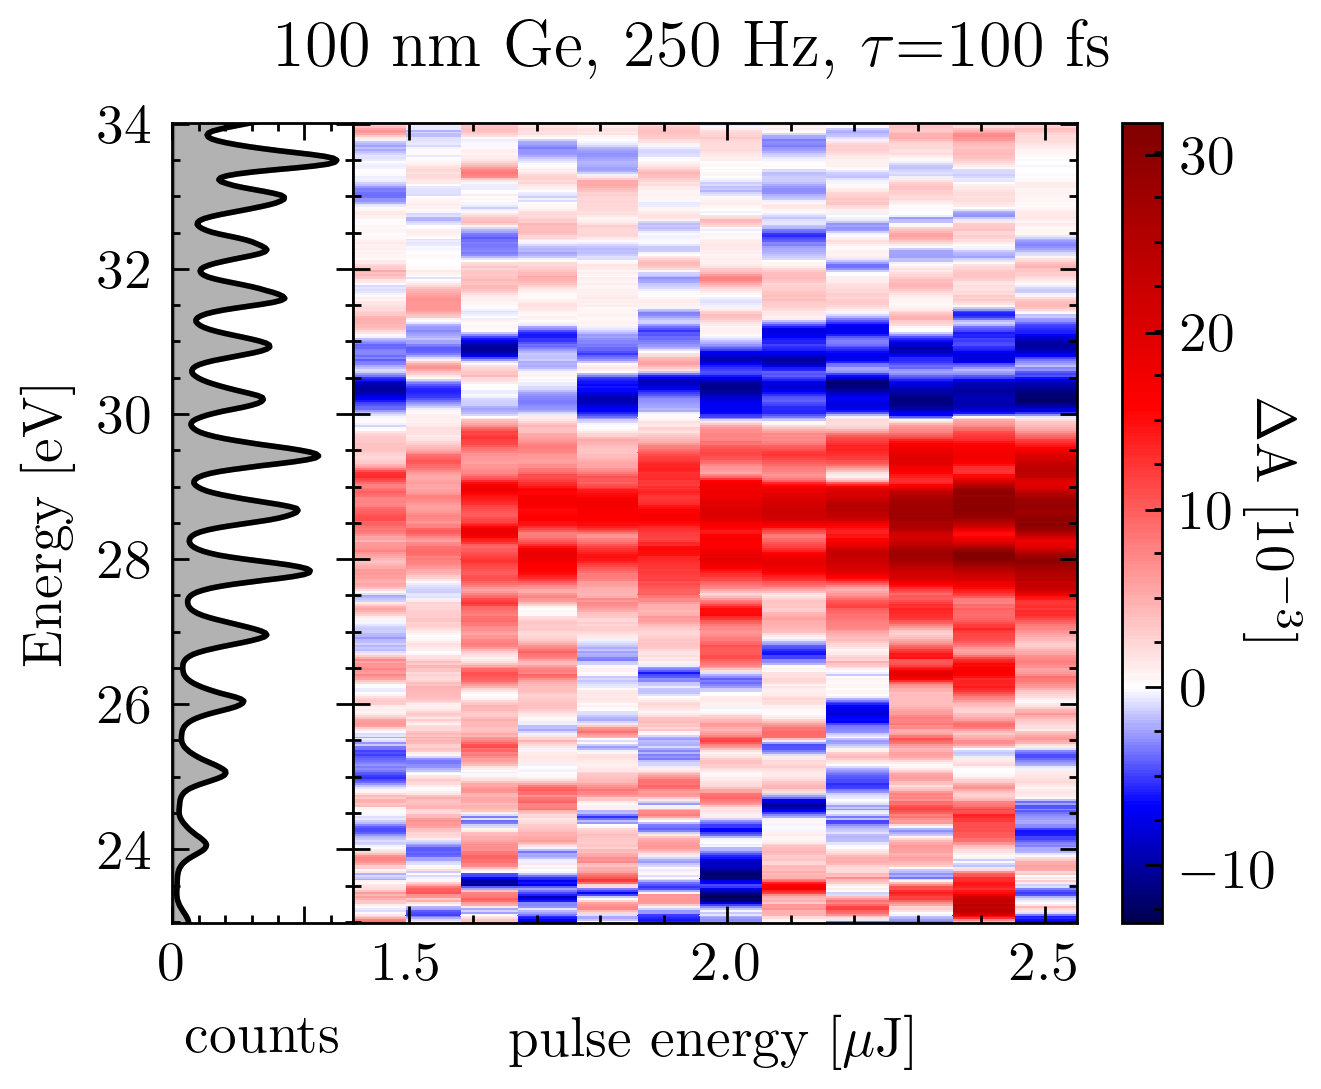
\includegraphics[width=0.75\textwidth]{figures/chap3/Ge_power_scan_20190911.png}
	\caption{Pulse energy scan of 100 nm germanium sample near temporal overlap. Left panel shows the average ground state spectrum, $S_{gs}(E)$. Right panel shows the change in absorbance, $\Delta A(E, PE)$, as a function of pulse energy, $PE$. Data shown in this figure is the average of 20 identical measurements: individual datasets were background subtracted and normalized for exposure time before being averaged; no additional data processing was performed on this dataset. See text for details.}
	\label{fig:Ge_power_scan}
	% dataset: C:\testdata\2019_09_11\HWP1
	% python file: ODcalc_HWP_averaging.py
	% how i got the pulse energy: we recorded LeCroy pkpk for 2 values of HWP (min, max). i used TDS-LeCroy conversion file to convert this to TDSmean values, and then the 2019-07-26 HWP calibration to convert it to pulse energy [microJ]. this gave me a min and max value of the pulse energy. for the rest of the points, i fit HWP vs power meter data (2019-07-26 HWP data) to get the cos()^2 curve, then scaled it vertically using the min,max power datapoints to convert them to pulse energy.
\end{figure}

The rep. rate was lowered to either 250 or 125 Hz

avg power and pulse energy where damage occurs vs. rep rate (sample=?, $\lambda$=?):
1000 Hz:
500 Hz:
250 Hz:
125 Hz:

only see time dependence at 125 and 250 Hz.

\begin{enumerate}
	\item hitting the samples too hard makes them pop (usually). sometimes, only a hole is drilled in the sample. this means that we have to be very careful when figuring out which power to use. it's very easy to destroy all your samples in an afternoon!
	\item discuss role of avg power and rep rate in sample damage. i.e., why we went to 250 and 125 Hz.
	\item plot $\Delta A$ vs. pump arm power
	\item conclude with the average pulse energy and rep rate settings that we used
\end{enumerate}


Ge-specific experimental parameters: wavelength, generation conditions, exposure time, MCP settings, rep rate, etc.

calculated excitation percentage, from lens calculations and measured IR power.

does the measured signal strength make sense? i.e., order of magnitude

show pictures of popped membranes. show delay spectrograms of drilled out samples.


Laser induced sample damage can occur from high intensities or from high average power. Regardless of the mechanism, the entire membrane is usually destroyed when a single point is laser drilled. 

you can talk about high average power damage and high peak power damage. no plots, but maybe mention the parameters that led you to believe that you were operating at the boundary between those two regimes.

\subsubsection{HM2 optimization}


also talk about HM2 optimization using harmonic signal. 

\section{50 nm Ge measurements}
i think we have a dataset or two showing a weak signal.


\section{100 nm Ge measurements}
we went to 100 nm because the 50 nm was too weak.

$N=50$ dataset experimental parameters: $\lambda$ = 1430 nm, Spitfire rep. rate = 125 Hz, pump energy (before focusing optics) $\sim$ 2.9 $\mu$J per pulse, camera exposure time = 3 seconds. each run took about 6 minutes for a total collection time of about 5 hours. 

\begin{figure}
	\centering
	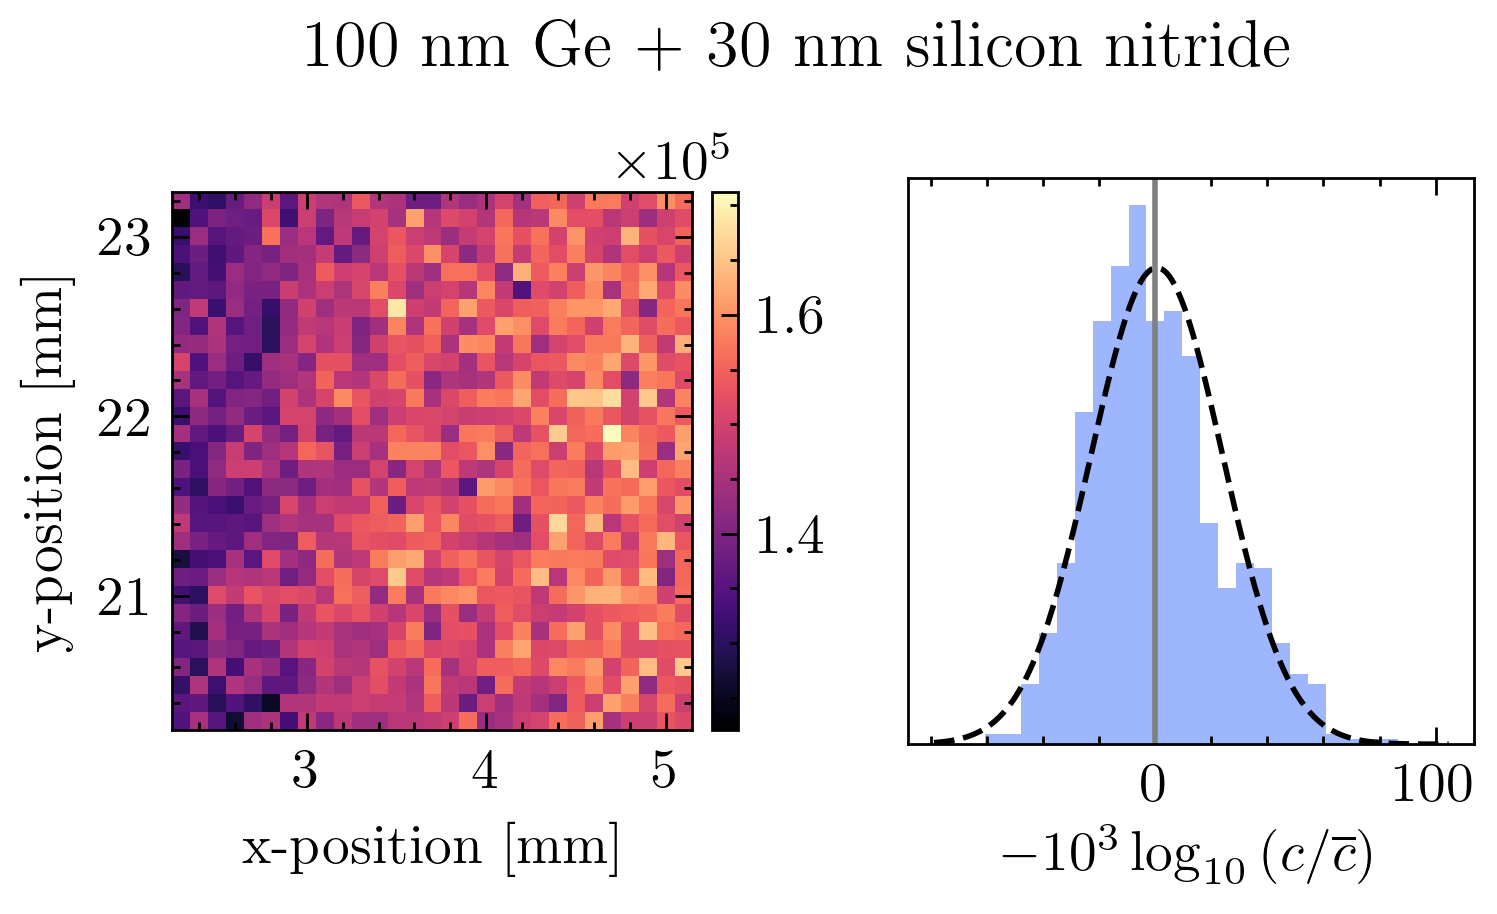
\includegraphics[width=0.75\textwidth]{figures/chap3/Ge_map.png}
	\caption{Left panel: spatial mapping of integrated XUV counts \textbf{(integrated over what energy range?)} of a 100 nm Ge + 30 nm silicon nitride sample. Right panel: histogram of values from the left panel.}
	\label{fig:Ge_map}
		% figure created using \Python Scripts\Spectrometer\test\rastermap.py
	% dataset: C:\testdata\2019_08_27\11_26_52 AM_Ge7_map1
\end{figure}

\section{Data Processing}

\begin{figure}
	\centering
	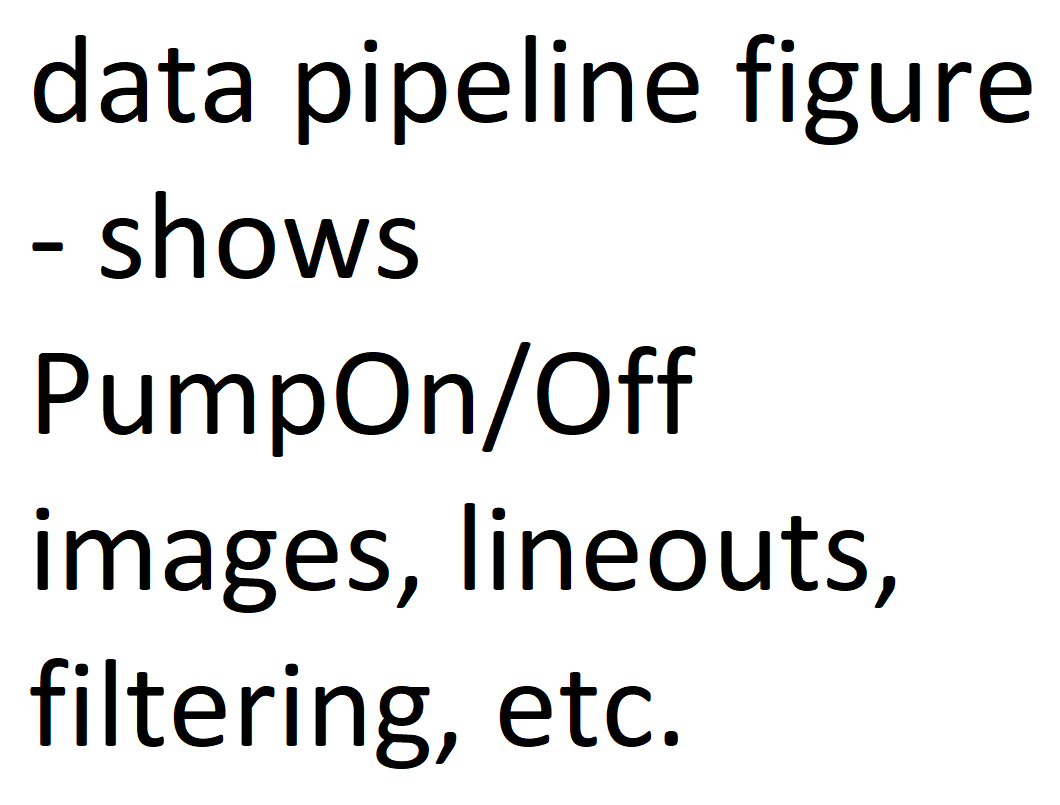
\includegraphics[width=0.5\textwidth]{figures/chap3/Data_Pipeline.png}
	\caption{this figure shows the data processing pipeline. it shows how we start with PumpOn-Off 2D images and transform them into spectrograms. it includes steps like an absorbance (A) calculation, spectral lineouts, frequency filtering and smooth, energy calibration, etc.}
	\label{fig:Data_Pipeline}
\end{figure}

\begin{figure}
	\centering
	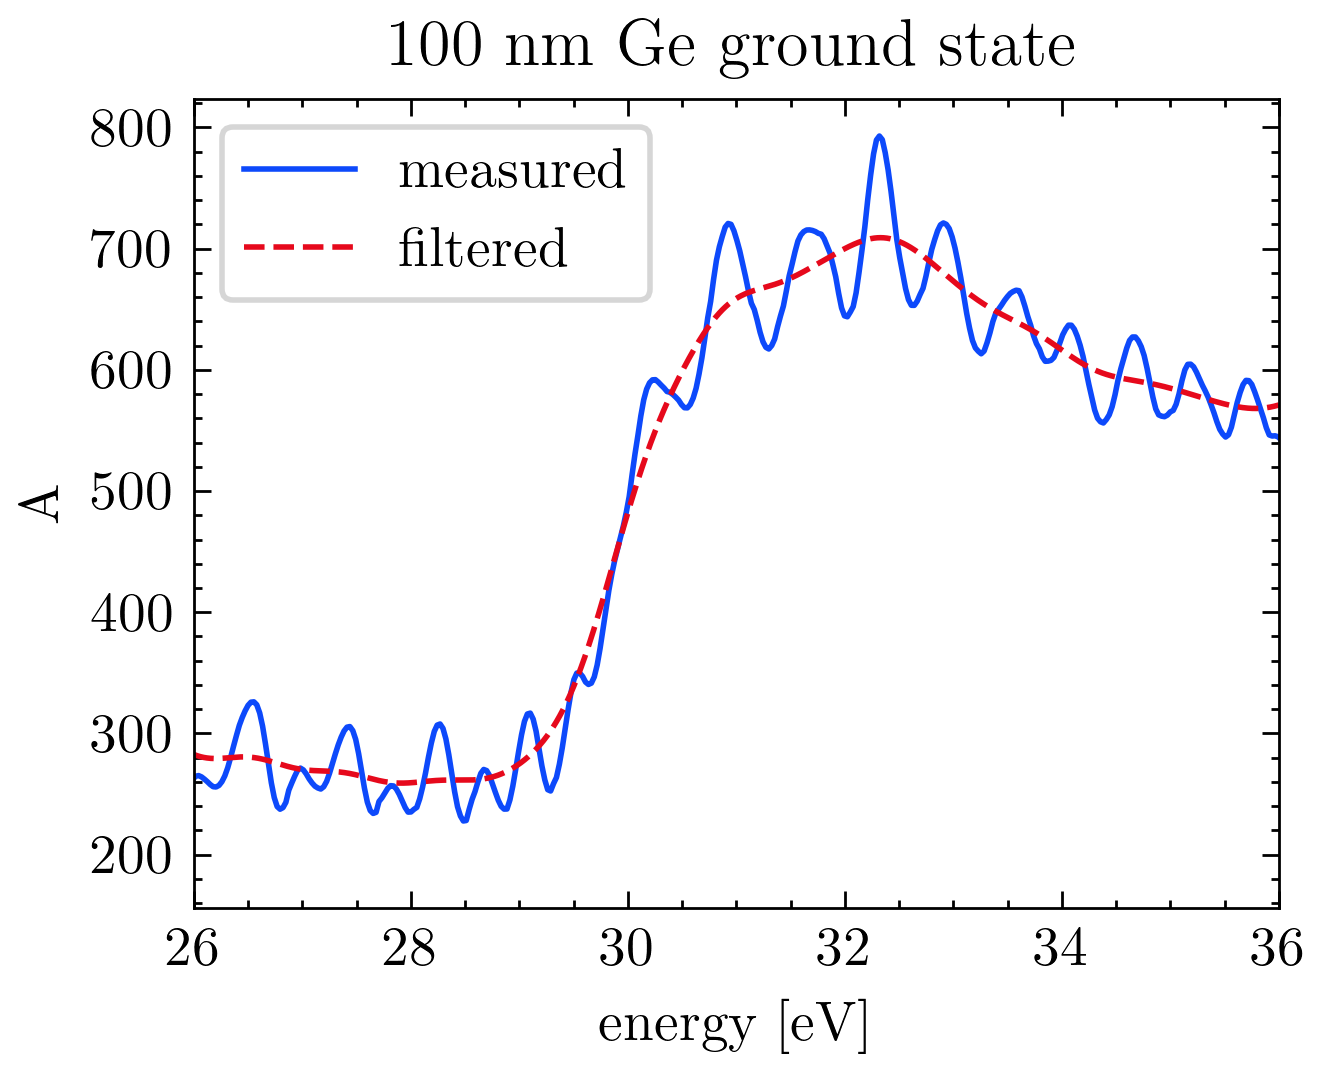
\includegraphics[width=0.5\textwidth]{figures/chap3/Ge_100nm_ground_state.png}
	\caption{this figure shows the ground state $A$ of 100 nm germanium.}
	\label{fig:Ge_100nm_ground_state}
	% data set: ???
	% figure made using: ???
\end{figure}

\begin{figure}
	\centering
	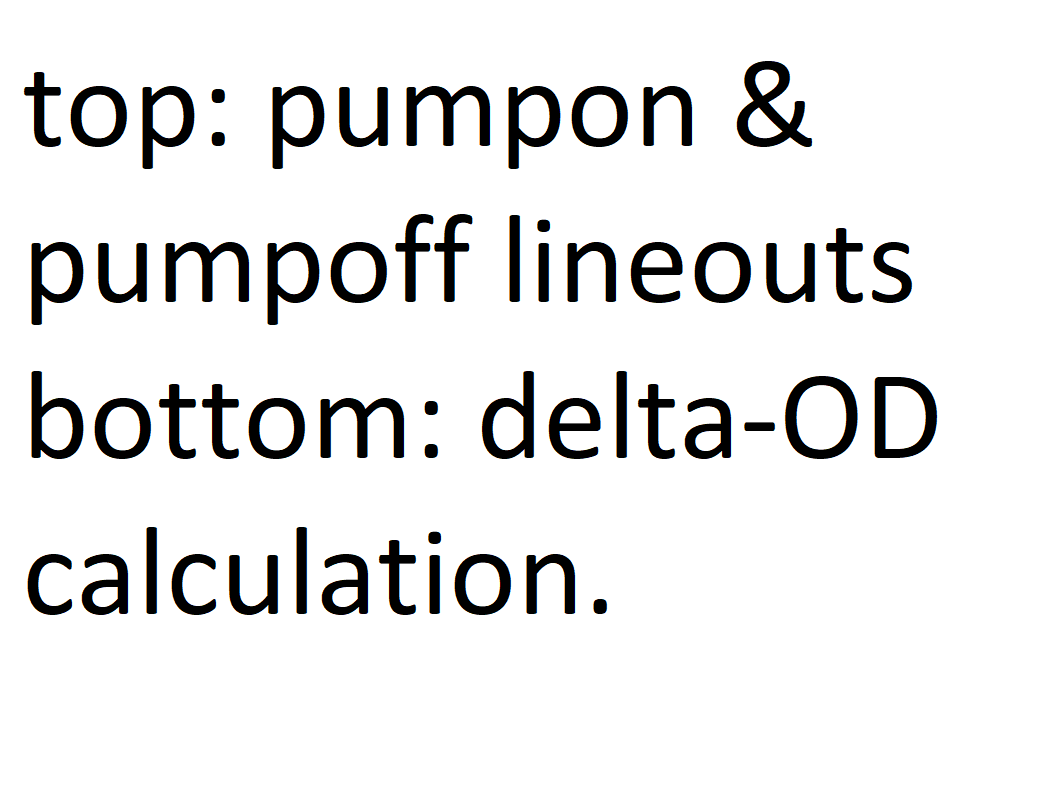
\includegraphics[width=0.5\textwidth]{figures/chap3/PumpOn_vs_PumpOff.png}
	\caption{this figure shows, using real data, a pump off and pump on spectral lineout. in another panel, it shows the $\Delta A$.}
	\label{fig:PumpOn_vs_PumpOff}
	% data set: ???
	% figure made using: ???
\end{figure}

\begin{figure}
	\centering
	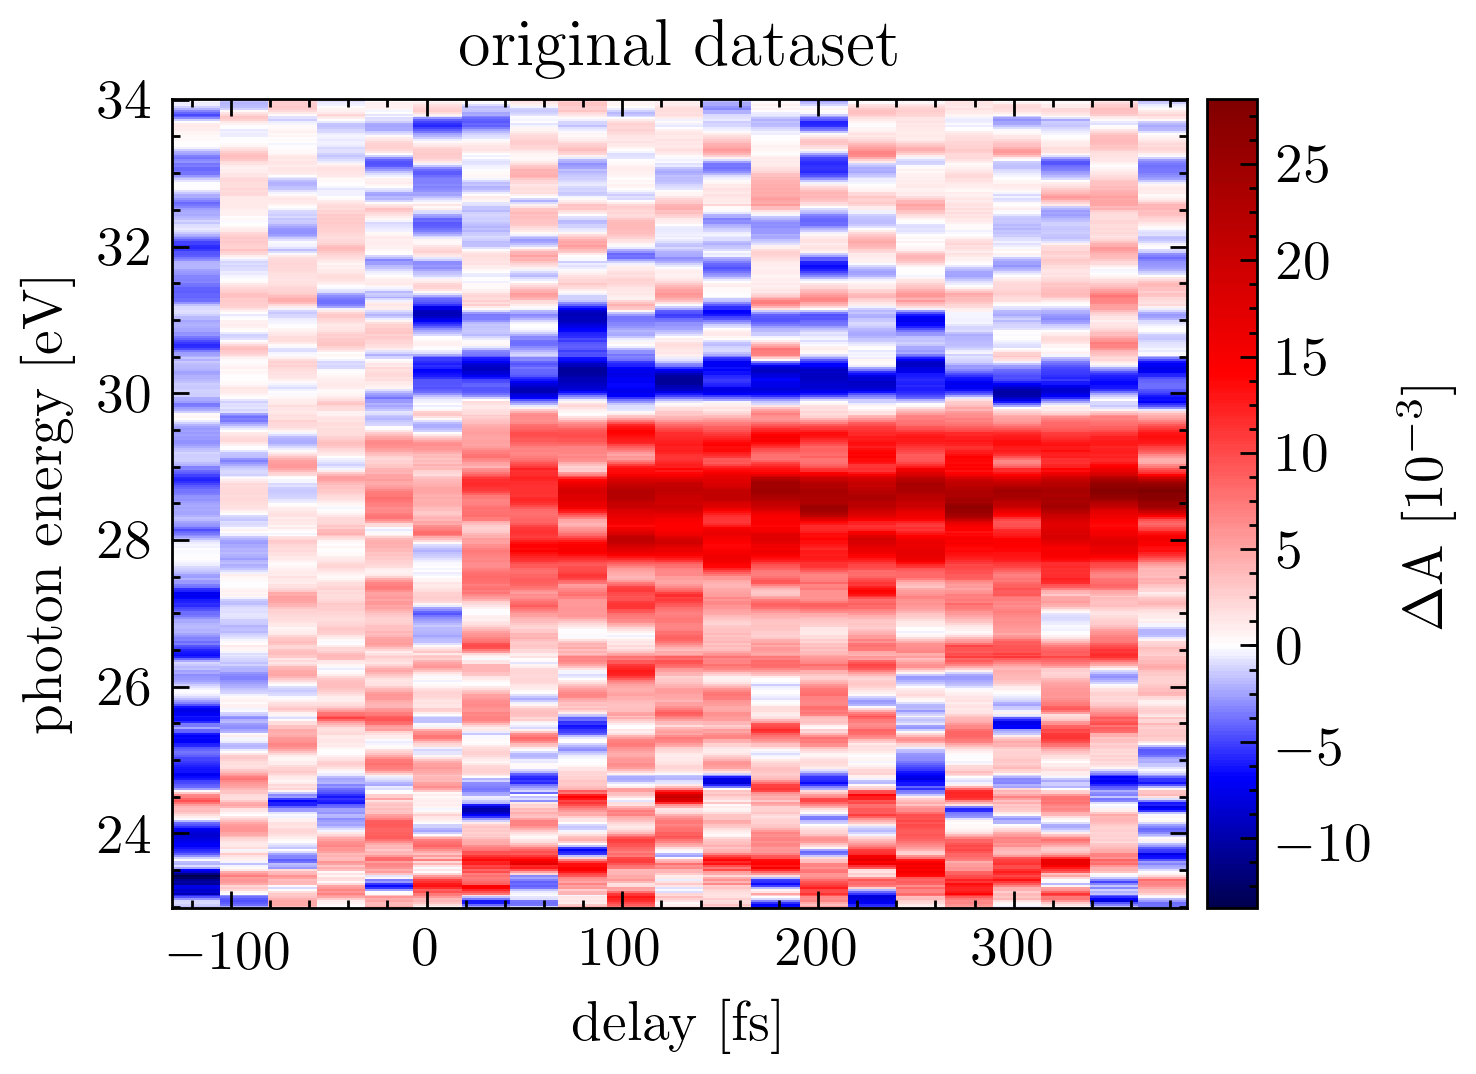
\includegraphics[width=0.5\textwidth]{figures/chap3/Ge_uncorrected_raw_spectrogram.png}
	\caption{$N=50$ averaged delay scans. no corrections have been made to the data}
	\label{fig:Ge_uncorrected_raw_spectrogram}
	% data set: ???
	% figure made using: ???
\end{figure}

\begin{figure}
	\centering
	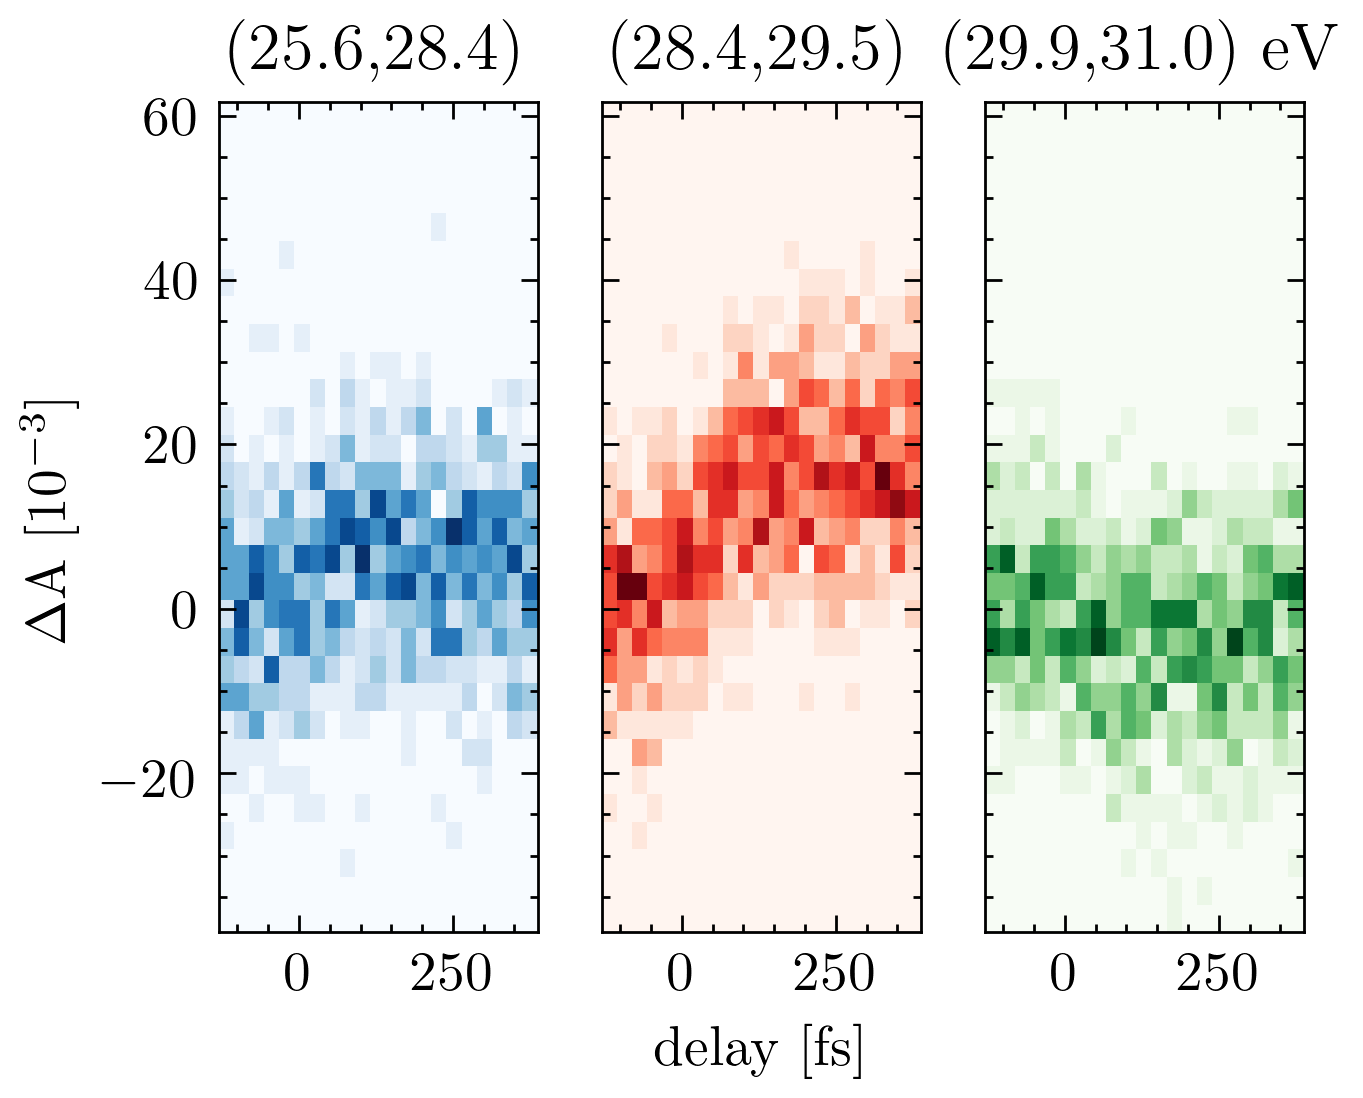
\includegraphics[width=0.5\textwidth]{figures/chap3/uncorrected_hist.png}
	\caption{$N=50$ averaged delay scans. no corrections have been made to the data. histogram of $\Delta A$ for 3 selected features. dataset is same as \cref{fig:Ge_uncorrected_raw_spectrogram}.}
	\label{fig:uncorrected_hist}
	% data set: ???
	% figure made using: ???
\end{figure}

\begin{figure}
	\centering
	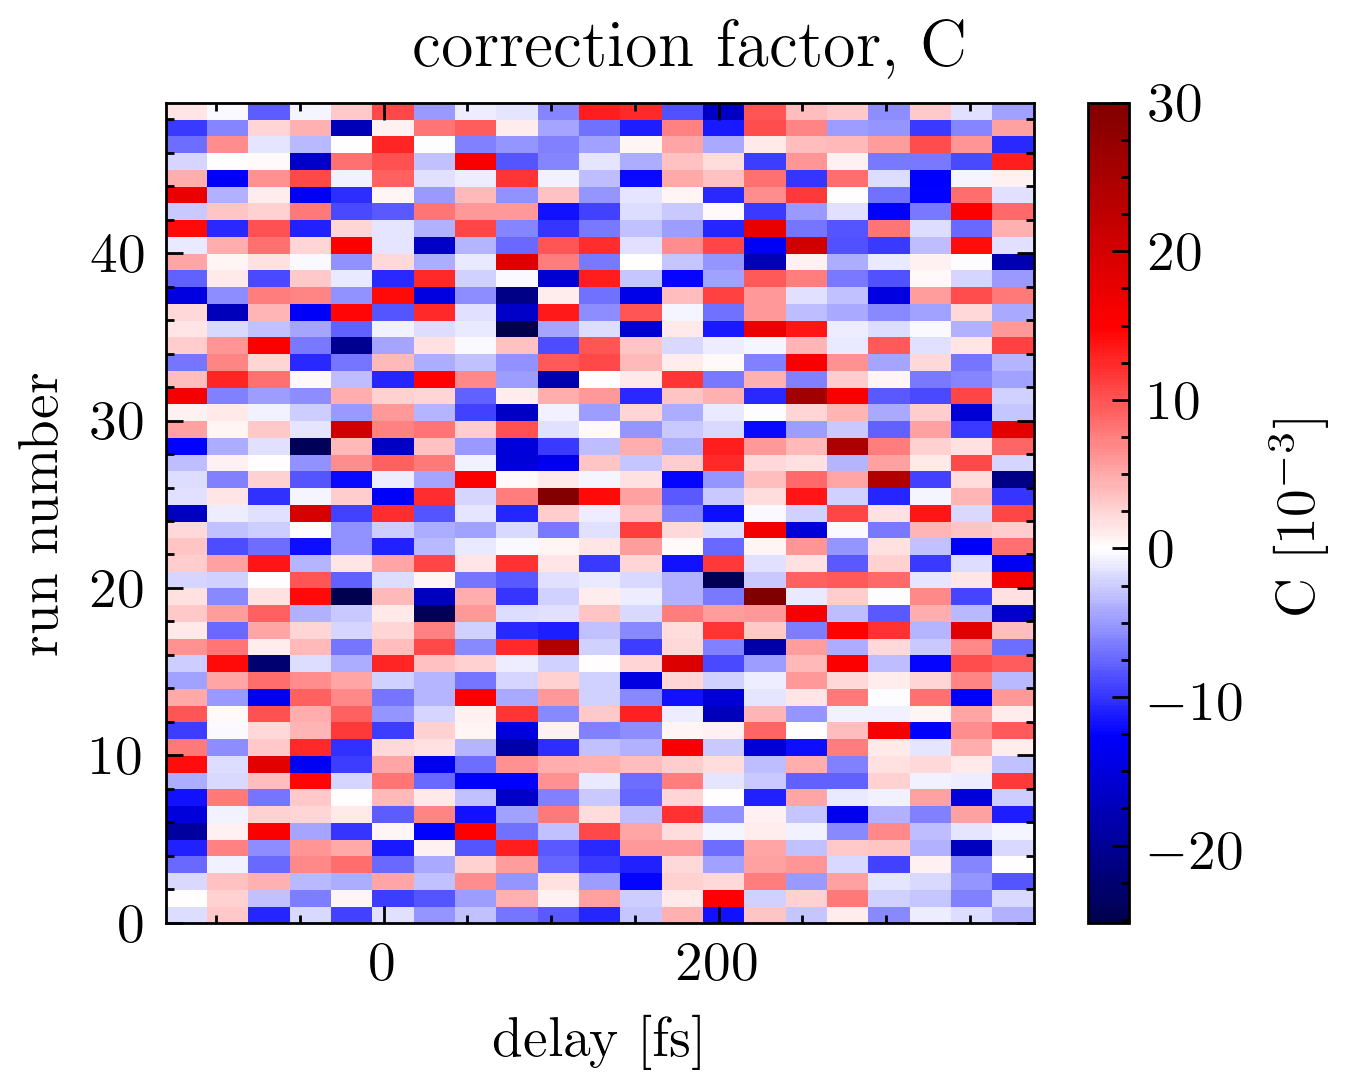
\includegraphics[width=0.5\textwidth]{figures/chap3/C_factor_image.png}
	\caption{correction factor, $C(\tau,E)$, from \cref{eqn:deltaA_linear_correction}.}
	\label{fig:C_factor_image}
	% data set: ???
	% figure made using: ???
\end{figure}

\begin{figure}
	\centering
	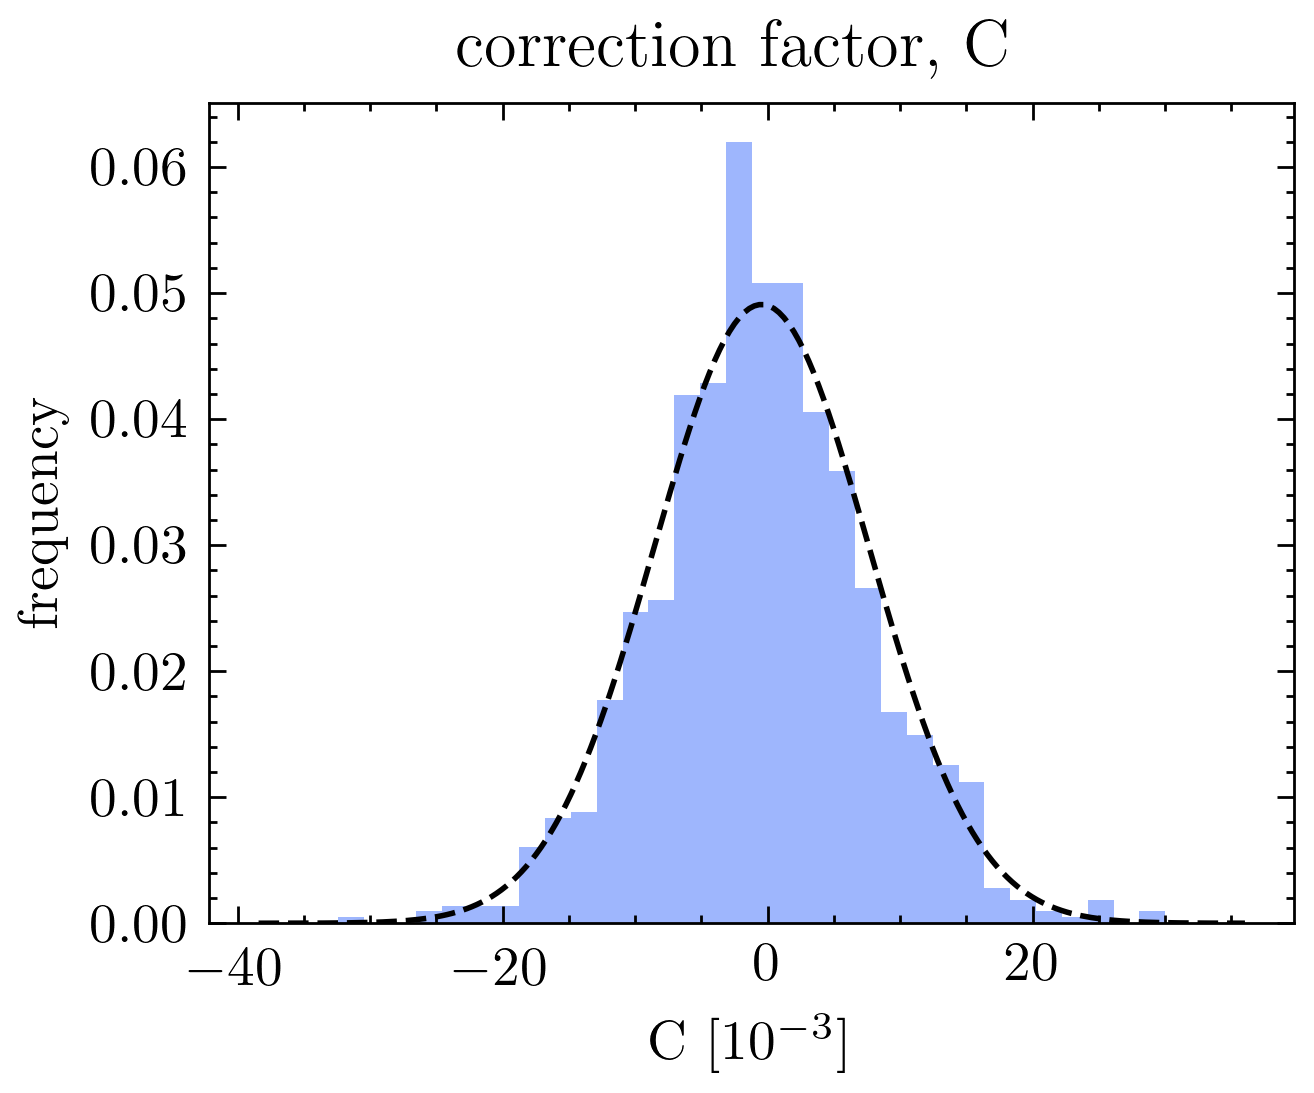
\includegraphics[width=0.5\textwidth]{figures/chap3/C_factor_hist.png}
	\caption{histogram of correction factor, $C(\tau,E)$, values from \cref{eqn:deltaA_linear_correction}.}
	\label{fig:C_factor_hist}
	% data set: ???
	% figure made using: ???
\end{figure}

\begin{figure}
	\centering
	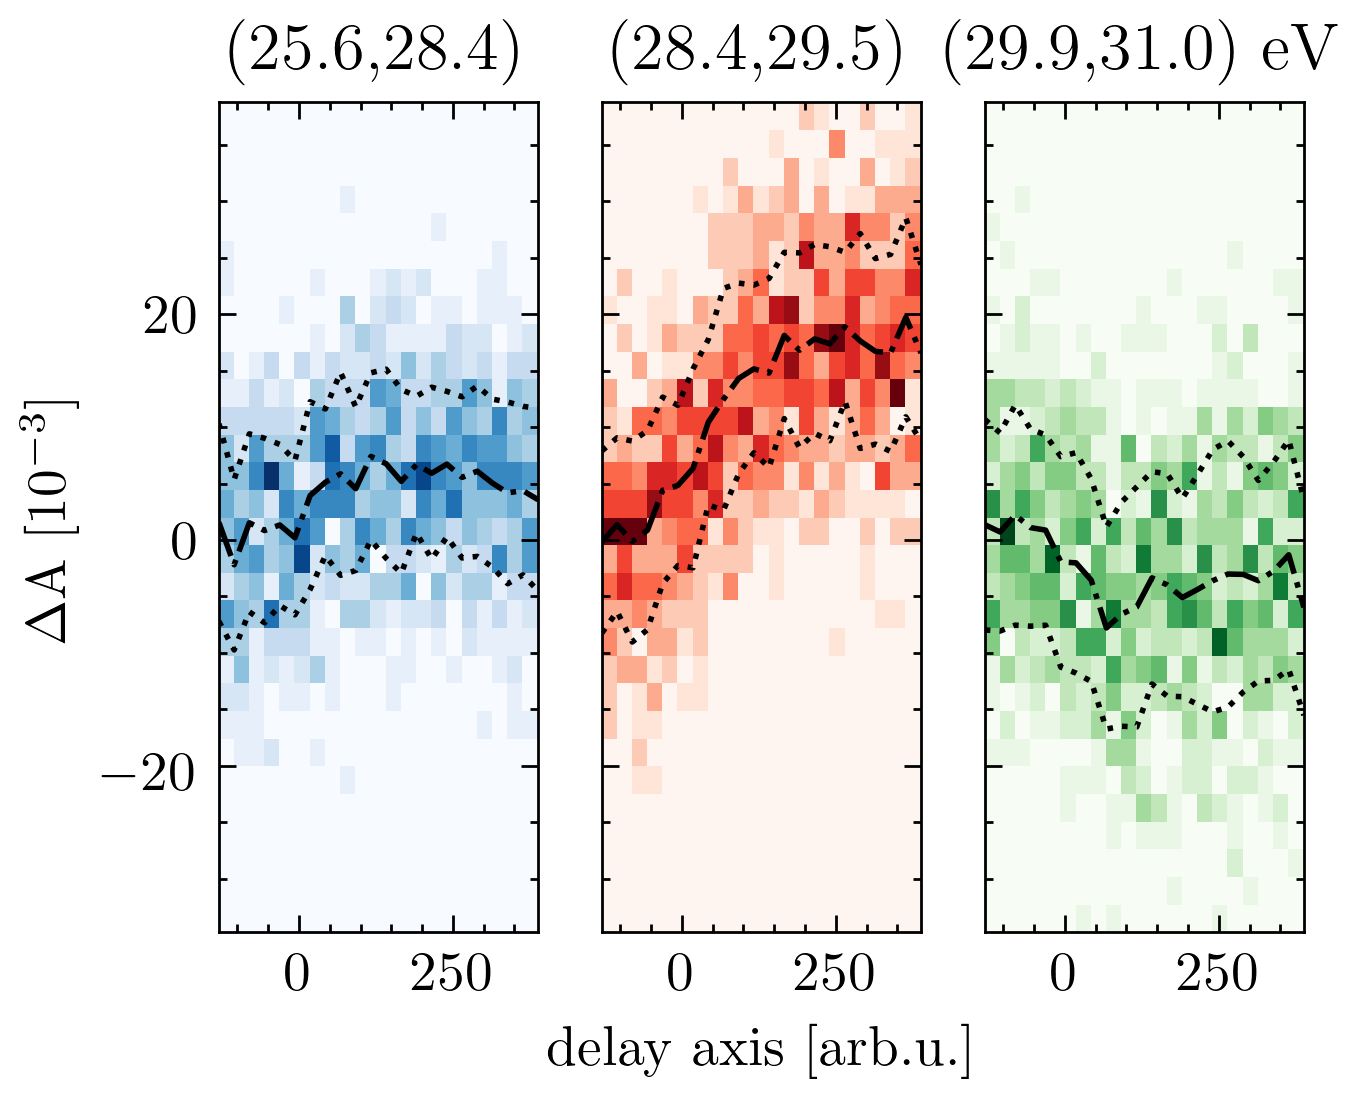
\includegraphics[width=0.5\textwidth]{figures/chap3/corrected_hist.png}
	\caption{histogram of spectral features from dataset with correction factor $C(\tau,E)$ applied }
	\label{fig:corrected_hist}
	% data set: ???
	% figure made using: ???
\end{figure}

\begin{figure}
	\centering
	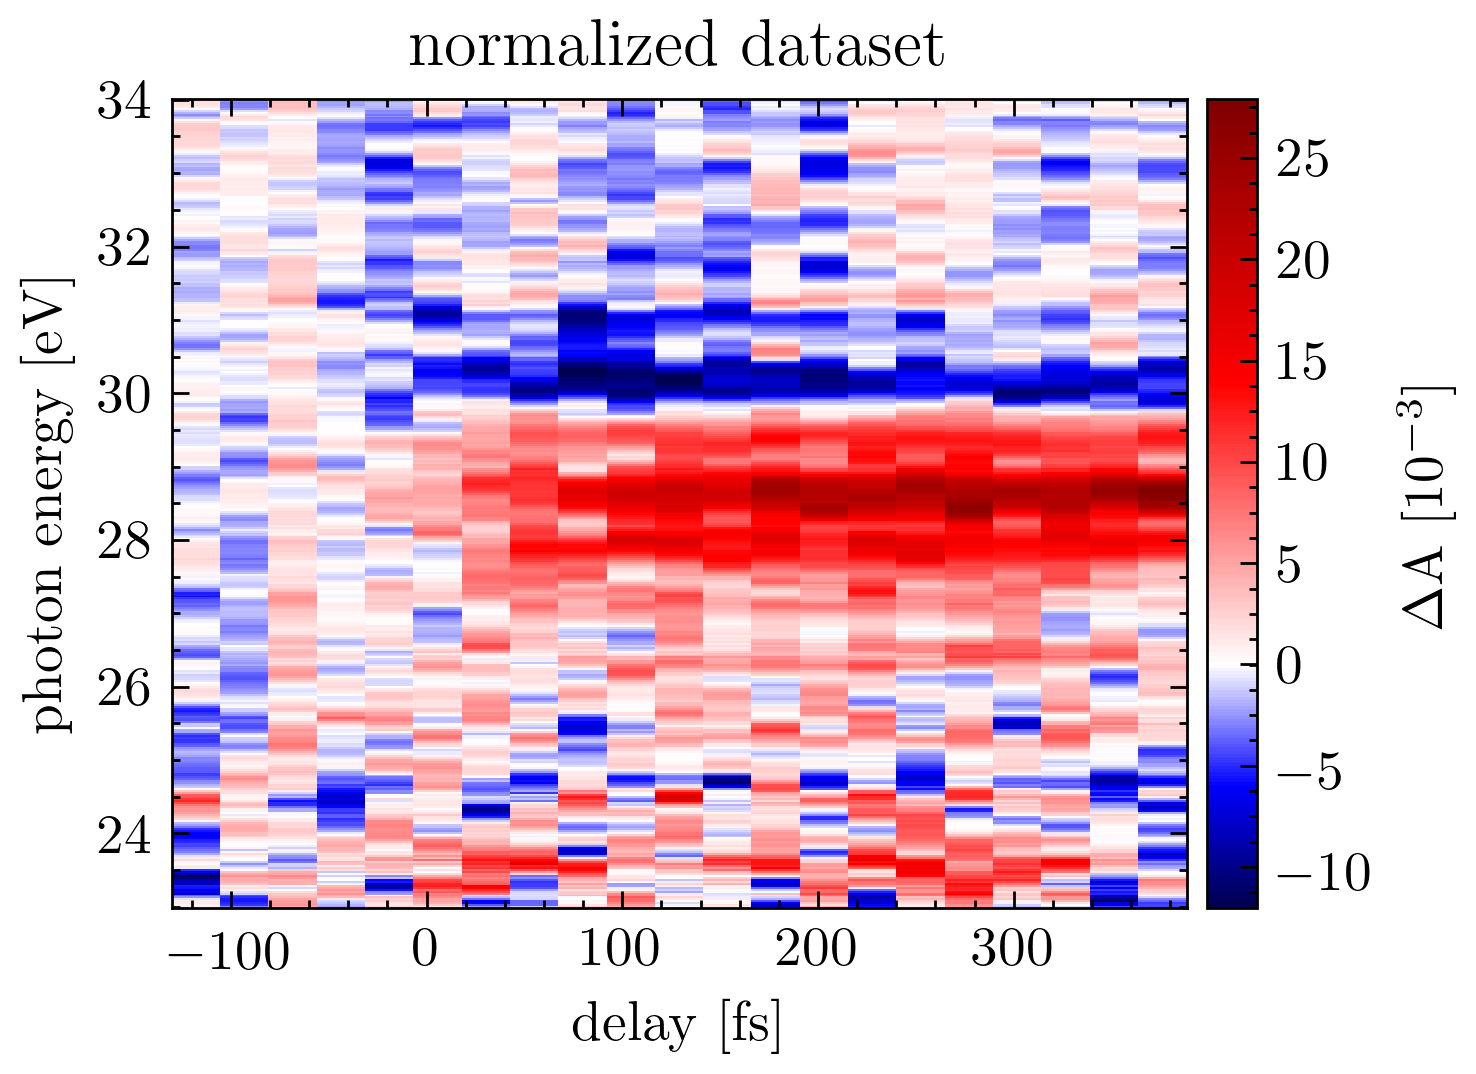
\includegraphics[width=0.5\textwidth]{figures/chap3/Ge_corrected_raw_spectrogram.png}
	\caption{normalized dataset: dataset with correction factor $C(\tau,E)$ applied }
	\label{fig:Ge_corrected_raw_spectrogram}
	% data set: ???
	% figure made using: ???
\end{figure}

\begin{figure}
	\centering
	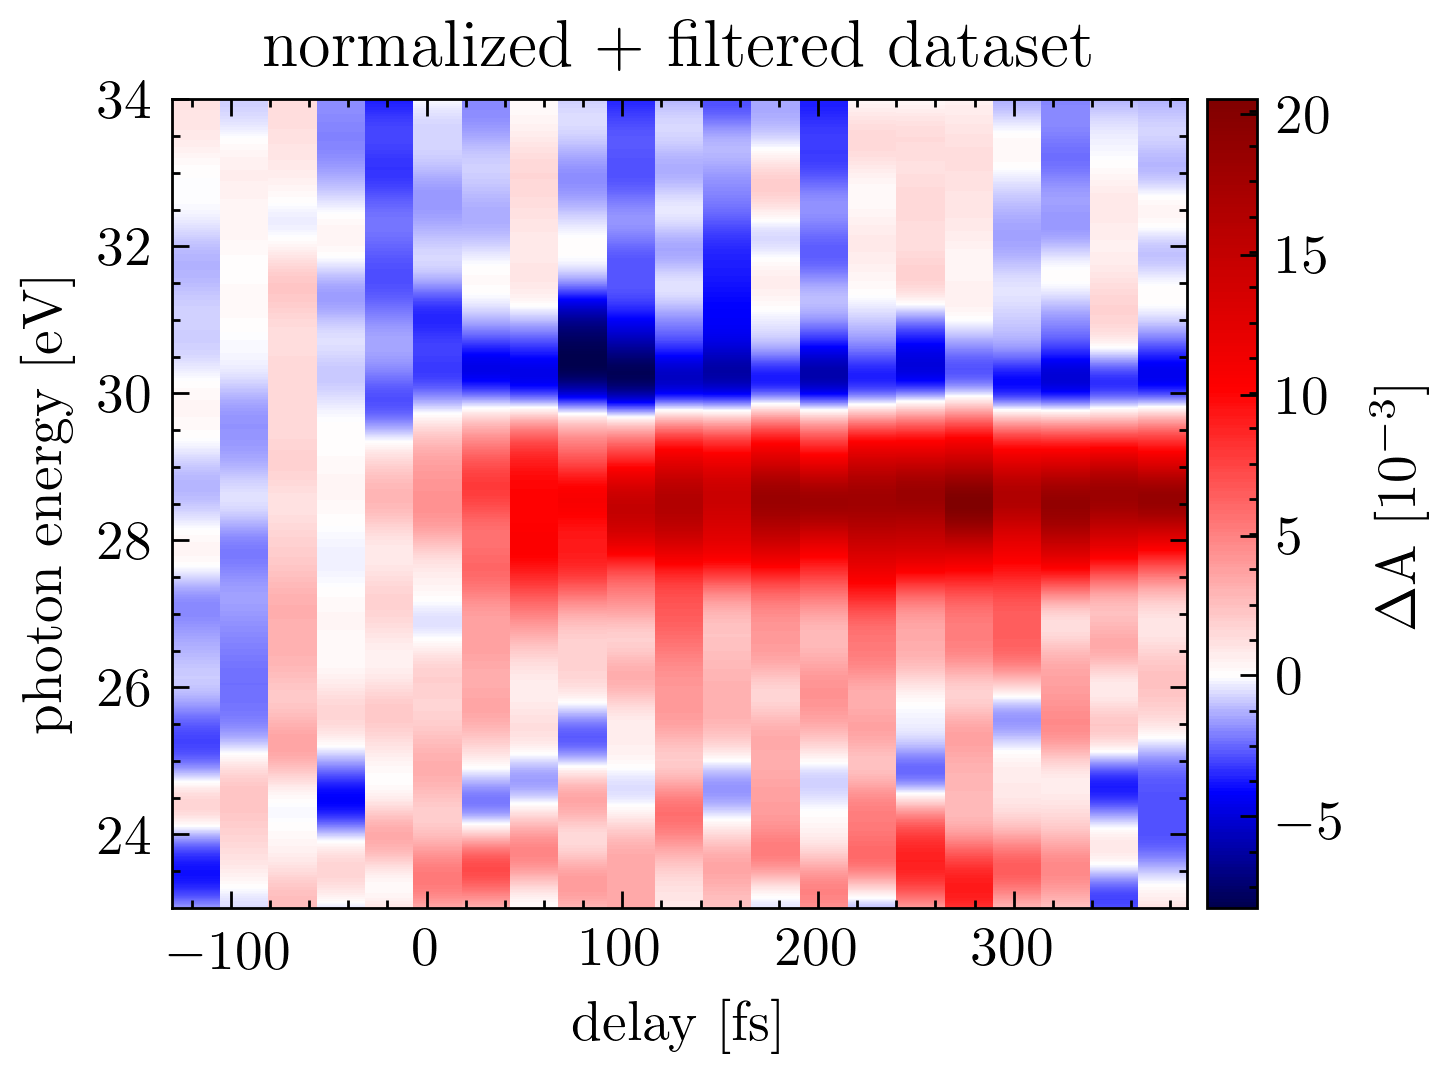
\includegraphics[width=0.5\textwidth]{figures/chap3/Ge_corrected_filtered_spectrogram.png}
	\caption{normalized dataset with frequency filter applied }
	\label{fig:Ge_corrected_filtered_spectrogram}
	% data set: ???
	% figure made using: ???
\end{figure}


The XUV photon spectrometer utilizes a flat field grating (Hitachi, 1200 l/mm) to spectrally disperse the XUV light. The grating is designed to focus along the spectral axis (horizontal direction of sensor) while preserving the spatial profile of the beam (vertical direction). The focus of the grating is incident on a 75 mm diameter imaging quality microchannel plate (MCP) array (Photonis), which converts the XUV photons into electrons via a nonlinear avalanche process with a gain of approximately $10^6 - 10^8$. These electrons are accelerated towards a phosphor screen, which converts the electrons into visible photons with a central wavelength of $\sim480$ nm. The visible photons exit the vacuum chamber via a glass feedthrough and are imaged by a lens onto a CMOS sensor of a digital camera (Andor). The recorded data is a two dimensional array of counts, with the horizontal axis representing the spectral content and the vertical axis representing the spatial profile of the beam.

talk about all the steps you use to process the data, starting from the 2d image and ending with the delta-A spectrogram.

\begin{enumerate}
	\item calibration of spectrometer energy axis and delay axis (just state it as fact, don't go into detail)
	\item data reduction: 2D image to 1D spectral lineout for each measurement. note that the jacobian needs to be used for plotting counts vs energy, but not for $\Delta A$ or $A$ since it divides out
	\item investigation of noise: peaks vs valleys vs slopes of harmonics. most of the noise comes from not the peaks, so we use the value at the peak for later analysis
	\item sample drilling or harmonic drift? inconclusive? or \textit{no conclusive evidence of drilling?}
	\item correlations between different harmonic peaks in $\Delta A$
	\item linear correction method $C(\tau,E)$
	\item choice of dx=2 method
	\item frequency filtering
	\item failed methods: SVD, interpolation
\end{enumerate}

\subsection{energy and delay calibration}
\subsection{A note about the Jacobian}

At each pixel, the spectrometer's camera records the integrated counts within the area of one pixel. We wish to convert the measured dataset (counts \textit{vs.} spectral pixel) to a physically meaningful spectrum (counts \textit{vs.} photon energy) while conserving energy \cite{mooneyGetBasicsRight2013}.

More precisely, our measurement samples a counts function $f_p$ in the spectral pixel basis $p$:
\begin{equation}
f_p (p): \text{spectral pixel} \rightarrow \text{counts}.
\end{equation}
The spectral pixel value is proportional to wavelength, with some extra factors that account for the geometry of the detector relative to the grating. We can convert the domain of the spectrometer's dataset from spectral pixels $p$ to energy $E$ (in eV) using an invertible polynomial transformation\footnote{The details surrounding the choice of this transformation will be discussed elsewhere in the dissertation.}:
\begin{equation}
\begin{aligned}
E(p)&: \text{spectral pixel} \rightarrow \text{energy [eV]}, \\
E(p) &= a_4 p^2 + a_3 p^3 + a_2 p^2 + a_1 p + a_0.
\end{aligned}
\end{equation}
Let the inverse of $E(p)$ be $p(E)$. From energy conservation, the transformation must preserve the integrated counts:
\begin{equation}
f_p(p) \text{ } dp = f_E(E) \text{ } dE.
\end{equation}
Rearranging, we obtain an expression for the counts expressed in the energy domain, $f_E$:
\begin{equation}
f_E (E) = f_p (p) \frac{dp}{dE} = f_p(p) \frac{d}{dE} p(E).
\label{eqn:spectrometer_jacobian}
\end{equation}
Therfore, the measured spectrum $f_p(p)$ in the pixel basis can be converted to the energy basis by multiplying it by a factor of $\frac{d}{dE} p(E)$. Note that this factor is only important when considering spectrometer counts; calculations of $A$ or $\Delta A$ can omit the Jacobian as it is common to both spectra and will divide out.

\subsection{source of noise}
\subsection{sample drilling or random drift?}
\subsection{correlations between harmonic peaks in $\Delta A$}
\subsection{integration vs summation near harmonic peaks}
\subsection{apparent $\omega$ and $2\omega$ oscillations in data}



mention calibration of spectrometer in passing, 2D image $\rightarrow$ 1D spectrum. jacobian needs to be used for plotting counts vs energy, but not for delta-OD, OD or transmission figures.

\begin{equation}
\Delta A^{\text{meas}}(\tau, E) = -\log_{10} \left( \frac{I_{on} f}{I_{off}} \right) = \Delta A^{\text{norm}}(\tau,E) + C(\tau,E)
\label{eqn:deltaA_linear_correction}
\end{equation}
